% ------ BEGIN PREAMBEL ------
\documentclass[a4paper,10pt, bibliography=totocnumbered]{scrreprt}

\usepackage[utf8x]{inputenc}
\usepackage[english]{babel}

\usepackage{graphicx}
\usepackage{pdfpages}
%\usepackage{subfig}
%\usepackage{microtype}
\usepackage{tabularx}
%\usepackage{amsmath, textcomp}

% Custom packages
\usepackage[numbers]{natbib}
\usepackage{longtable}
\usepackage{ragged2e}
%\usepackage{tikz}
%\usetikzlibrary{positioning}
%\usepackage{pdflscape}
%\usepackage{rotating}

\usepackage{csquotes}
\usepackage{listings}
\usepackage{booktabs}
\usepackage{tablefootnote}
\usepackage{float}

% Links
\usepackage{hyperref}
\hypersetup{
    colorlinks=true,        % false: boxed links; true: colored links
    linkcolor=black,        % color of internal links
%    citecolor=green,        % color of links to bibliography
    citecolor=black,        % color of links to bibliography
    filecolor=magenta,      % color of file links
    urlcolor=blue           % color of external links
}

% Glossary
\usepackage[nomain,acronym,toc]{glossaries} 
\makeglossaries
\newglossaryentry{Contract}
{
	name={Contract},
	description={A requirement-level logical expression used to express preconditions and postconditions of an \textit{operation}.}
}

\newglossaryentry{Coverage criterion}
{
	name={Coverage criterion},
	description={A criterion used to limit the amount of \textit{test objectives} to be generated. Specifies which paths to traverse in the context of the traversal of a \textit{transition system}.}
}

\newglossaryentry{Interaction Overview Diagram (IOD)}
{
	name={Interaction Overview Diagram (IOD)},
	description={A special form of activity diagram used to show control flow. Each node in the IOD represents either an interaction diagram (sequence diagrams) or interaction occurrences that show an \textit{operation} invocation.}
}

\newglossaryentry{Object Constraint Language (OCL)}
{
	name={Object Constraint Language (OCL)},
	description={A declarative language in the UML standard used to define \textit{contracts}.}
}

\newglossaryentry{Operation}
{
	name={Operation},
	description={An abstract term used to describe a state transition in a \textit{transition system}. Is equal to a \textit{use case} in \cite{ClementineNebut2006} or to an interaction diagram/interaction occurrence in \cite{NajlaRaza2007}.}
}

\newglossaryentry{Test case}
{
	name={Test case},
	description={Tests a single \textit{use case}.}
}

\newglossaryentry{Test objective}
{
	name={Test objective},
	description={A synonym for test path as a combination of abstract \textit{operations} to be composed into one \textit{test scenario}.}
}

\newglossaryentry{Test scenario}
{
	name={Test scenario},
	description={A sequential composition of \textit{test cases}.}
}

\newglossaryentry{Transition system}
{
	name={Transition system},
	description={Used to derive \textit{test scenarios} by helping to generate \textit{test objectives} through its traversal. Consists of states and transitions, where states are given by \textit{contracts} and transitions are given by \textit{operations}.}
}

\newglossaryentry{UC-System}
{
	name={UC-System},
	description={A prototype/interpreter-tool used to build a \textit{transition system} in \cite{ClementineNebut2006} and to derive \textit{test objectives} from it.}
}

\newglossaryentry{UC-SCSystem}
{
	name={UC-SCSystem},
	description={A prototype-tool using \textit{use case scenarios} to derive executable \textit{test scenarios} as JUnit tests in \cite{ClementineNebut2006}.}
}

\newglossaryentry{Use case}
{
	name={Use case},
	description={An abstract, requirement-level term used to describe a main functionality of a system.}
}

\newglossaryentry{Use case scenario}
{
	name={Use case},
	description={A synonym for sequence diagram in case of \cite{ClementineNebut2006}.}
}

\newglossaryentry{XML Metadata Interchange (XMI)}
{
	name={XML Metadata Interchange (XMI)},
	description={XML based metadata interchange format gained from an \textit{Interaction Overview Diagram} in \cite{NajlaRaza2007} to generate a \textit{transition system}.}
}

\setacronymstyle{long-short}
\newacronym{ex}{sample}{example}
\newacronym{NFR}{NFR}{non-functional requirement}
\newacronym{FR}{FR}{functional requirement}
\newacronym{UML}{UML}{uniform modeling language}


% ------ BEGIN EDINGER PACKAGES ------
\usepackage{listings}
\usepackage{xcolor}
\usepackage{array}
\usepackage{booktabs}
\newcommand{\tabitem}{~~\llap{\textbullet}~~}
\usepackage{multirow}
\usepackage{pdflscape}
\usepackage[pass]{geometry}

% define colors and configure listing
\colorlet{mygray}{black!30}
\colorlet{mygreen}{green!60!blue}
\colorlet{mymauve}{red!60!blue}
\lstset { %
	language=C++,
	backgroundcolor=\color{gray!10},  
	basicstyle=\ttfamily,
	columns=fullflexible,
	breakatwhitespace=false,      
	breaklines=true,                
	captionpos=t,                    
	commentstyle=\color{mygreen},
	emph={aspect, advice, pointcut, before, JoinPoint}, emphstyle={\color{blue}},
	extendedchars=true,              
	frame=single,                   
	keepspaces=true,             
	keywordstyle=\color{blue},      
	language=c++,                 
	numbers=none,                
	numbersep=5pt,                   
	numberstyle=\tiny\color{blue}, 
	rulecolor=\color{mygray},        
	showspaces=false,               
	showtabs=false,                 
	stepnumber=1,                  
	stringstyle=\color{mymauve},    
	tabsize=3,                      
	title=\lstname,
	numbers=left
}
% ------ END EDINGER PACKAGES ------

% ------ BEGIN HAUSBERGER PACKAGES ------
%\usepackage{csquotes}
%\usepackage{float}
\usepackage{longtable}
\usepackage{listings}
\usepackage{color}

\definecolor{dkgreen}{rgb}{0,0.6,0}
\definecolor{gray}{rgb}{0.5,0.5,0.5}
\definecolor{mauve}{rgb}{0.58,0,0.82}

\lstset{
	frame=tb,
	language=Java,
	aboveskip=3mm,
	belowskip=3mm,
	showstringspaces=false,
	columns=flexible,
	basicstyle={\small\ttfamily},
	morekeywords={UC, context, pre, @pre, post, and, or, not, implies, forall, exists},
	numbers=none,
	numberstyle=\tiny\color{gray},
	keywordstyle=\color{blue},
	commentstyle=\color{dkgreen},
	stringstyle=\color{mauve},
	breaklines=true,
	breakatwhitespace=true,
	tabsize=3
}
% ------ END HAUSBERGER PACKAGES ------
% ------ BEGIN KOCH PACKAGES ------
\usepackage[latin1]{inputenc}
\usepackage[a4paper]{geometry}
\geometry{verbose,tmargin=2cm,bmargin=2cm,lmargin=2.5cm,rmargin=2.5cm}
\setcounter{secnumdepth}{3}
\setcounter{tocdepth}{3}
\usepackage{babel}
\usepackage{array}
\usepackage{longtable}
\usepackage{float}
\usepackage{textcomp}
\usepackage{graphicx}
\usepackage[unicode=true,
 bookmarks=false,
 breaklinks=false,pdfborder={0 0 1},backref=section,colorlinks=false]
 {hyperref}
\hypersetup{pdftitle={Titel},
 pdfauthor={Autor},
 pdfpagelabels=true}
 
 % ------ END KOCH PACKAGES ------

% ------ END PREAMBEL ------

%% Title Page
\makeatletter
\renewcommand{\maketitle}{\begin{titlepage}
    \vskip 10\p@
    \hbox{
      \vrule depth 0.99\textheight
        \mbox{\hspace{2em}}
      \vtop{
        \vskip 10\p@
        \hspace{4pt}
        \vskip 50\p@
        \begin{flushleft}
          \Large \@author \par
        \end{flushleft}
        \vskip 50\p@
        \begin{flushleft}
          \huge \bfseries \@title \par
        \end{flushleft}
        \begin{flushleft}
          \Large \bfseries \@subtitle \par
        \end{flushleft}
        \vskip 70\p@
        \begin{flushleft}
          \Large \@publishers \par
        \end{flushleft}
        \vskip 50\p@
        \begin{flushleft}
          \Large \@date \par
        \end{flushleft}
        }}
  \end{titlepage}
}
\makeatother

\author{Author 1, Felix Hausberger, Max Edinger, Andre Meyering, Tobias Koch}
\title{Title }
\subtitle{Technical Report}
\publishers{\textbf{Advisor University of Heidelberg}\\ Prof. Dr. Barbara Paech, Astrid Rohmann}
\date{mm dd, year}



% Deutsche Absaetze:
\parindent 0pt
\parskip 12pt

\textwidth145mm
\setlength{\oddsidemargin}{0.7cm}
\setlength{\topmargin}{-0.5cm}
\setlength{\textheight}{22.5cm}

\begin{document}
\maketitle

\begin{abstract}
\section*{Abstract}

Testing is an essential and time-consuming part of any software development.
This work is a collaboration that highlights various approaches to how systematic tests can be created to make this process more efficient, clearer, easier or more successful.
After the introduction for this purpose eight different methods are dealt with in own subchapters.
Each of these chapters deals with the investigated approach, describes the problem, discusses the literature search on the topic, and then compares the approaches found in each case via a synthesis matrix.
The approaches are put into practice using the example of a movie manager.
Subsequently, the topic described in this subchapter is summarized and a statement regarding the usage for a systematic test generation is made. 

The first topic dealt with is \enquote{systematic generation of acceptance tests that are executable with FitNesse}.
It is about generating automatic tests with the tool FitNesse.
This approach tries to solve the difficulties of communication among the participants.
For this purpose several artifacts like the fit tables are created and used.
After the investigation, it is concluded that the approaches can work well depending on the project size and experience, but unfortunately it is highly dependent on the latter in particular. 

The next chapter discusses that it should be possible to generate test cases in early phases of development.
\enquote{Transition systems} can help to derive test cases from specifications.
The approaches examined here offer industry standard solutions, but the capability of generating robustness tests for fault detection is still a weakness.

The third subchapter deals with \enquote{Testing with a timing component}.
The difficulty of integrating individual software components into an overall project is described as a problem.
The aspect particularly considered here is the temporal component, since in many real-time systems the exact time between two instruction executions can lead to different results.
After an analysis, the conclusion is drawn that this is still a rarely used approach with many non-automated working steps. 

In the next chapter, approaches for model-based systems are examined.
First and foremost, these include \enquote{classification trees}.
The goal is to derive automatic test cases based on the requirements and the input parameters of a model.
In conclusion, classification trees are described as well arranged and close to the requirements, but can potentially produce many test cases.
Moreover, it is difficult to apply these approaches to systems without a simulated model.

The fifth subchapter focuses on \enquote{model based testing} and examines approaches to make testing with models better and describes the differences between system models and test models.
After the analysis the difficulties in using the tools given in literature are worked out.
Nevertheless, it is possible to reduce test time and errors by using them. 

The initial problem for the next chapter with \enquote{Testing functional and nonfunctional requirements in User Requirements Notation} is the risk for wrong test cases during manual test creation.
User requirements notation should fulfill requirements during test creation and thus prevent incorrect or incomplete tests.
At the end, the problem is discussed that this approach is largely unexplored.
Provided that one makes the effort to take additional steps in test case generation, one still achieves a better quality.

In \enquote{Testing Non-Functional Requirements with Risk Analysis} the focus is on risk analysis, because it is precisely here that error-prone components can be discovered.
Suitable approaches are then sought.
Among the findings here are the importance of automated tests and that tests for non-functional requirements should have more priority. 

The last chapter describes the \enquote{Testing Non-Functional Requirements with Aspects} and puts thereby in the comparison with the previous section the focus on the \enquote{aspects}.
This is intended to describe system-wide functionalities in order to be able to deal with concerns at system level.
Also here the missing availability of tools and suitable research are criticized.
However, the approaches considered seem promising and should be further refined.

Thus, this joint work addresses the merits and difficulties of various test case generation techniques.
Common problems identified are the lack of availability of tools or research, but in suitable use cases most approaches help in improving or automating the test cases.
A final conclusion on this is drawn at the end of this work.

\end{abstract}

\tableofcontents

\chapter{Introduction}\label{sec:introduction}

% Reviewfragen
% - Weckt die Einleitung das Interesse der LeserInnen am Thema?
% - Enthält die Einleitung eine detaillierte Problembeschreibung
%   der Herausforderungen in der Softwareentwicklung, die mit systematischer
%   Testerstellung adressiert werden sollen?
% - Enthält die Einleitung die wesentlichen Aussagen aus den Einleitungen der einzelnen Kapitel?

% Die Einleitung (1 Introduction) des Berichts soll das Interesse der LeserInnen
% am Thema wecken und die gemeinsamen Grundlagen beschreiben. Sie enthält eine
% detaillierte Problembeschreibung der Herausforderungen in der Softwareentwicklung,
% die durch systematische Testerstellung adressiert werden sollen. Zudem enthält sie
% die wesentlichen Aussagen aus den Einleitungen der einzelnen Kapitel 
\section{Systematic Software Testing}\label{sec:introduction_software_testing}

With the rise of smart gadgets and the Internet of Things, more and more parts of our daily life involve technology.
And the software required to run our smartphones, computers and other gadgets  becomes more complex as more data can be processed.
As software becomes more complex, bugs and even small configuration mistakes can have immense consequences as recent data breaches have shown\footnote{\enquote{235 Million Instagram, TikTok And YouTube User Profiles Exposed In Massive Data Leak}, \url{https://www.forbes.com/sites/daveywinder/2020/08/19/massive-data-leak235-million-instagram-tiktok-and-youtube-user-profiles-exposed/}, last visited on 2021-02-10}.
Furthermore, not testing software can have legal consequences.
If basic security measures are not implemented and tested, businesses may violate the \enquote{General Data Protection Regulation}\footnote{see \url{https://eur-lex.europa.eu/legal-content/EN/TXT/?uri=CELEX\%3A02016R0679-20160504&qid=1614251901149}, last visited on 2021-02-25}
(GDPR) and may have to pay fines.
This is not a hypothetical risk.
The \enquote{GDPR Enforcement Tracker}\footnote{see \url{https://www.enforcementtracker.com/}, last visited on 2021-02-10} lists instances where businesses had to pay fines due to \enquote{Insufficient technical and organisational measures to ensure information security}.

Therefore, proper testing of software becomes more important than ever.
But what is software testing? According to the \enquote{Guide to the Software Engineering Body of Knowledge} (short: SWEBOK), \enquote{Software testing consists of the dynamic verification that a program provides expected behaviors on a finite set of test cases, suitably selected from the usually infinite execution domain.}~\cite{SWEBOK}
This means that it may not even be possible to test every input against the expected output, for example if the input is an infinite data stream.
But also for functionality with a finite set of input data, testing every possible combination may not be feasible.
Software testing can take more time than developing the program under test. Hence, software testing can be tedious, difficult and expensive.
So the question arises how software can be tested in an effective and efficient way.

We need to write tests in a systematic way.
This paper contains 9~articles, % TODO: Hat einer aufgehört?
each describing another approach to systematic software testing.

In \autoref{sec:topic_2} % Fitnesse
we focus on acceptance tests with FitNesse.
Communicating requirements between customers and developers can be difficult.
Whereas natural language can be too ambiguous, code can be too technical.
By using FitNesse, human-readable Fit-Tables which include test steps are created that can be understood by customers. By writing fixture classes, these Fit-Tables can be used to automatically run tests.

But having tests may not be enough.
Which requirement is covered by which test?
Can we be sure that the implementation matches the specification?
Traceability becomes necessary and is required to not loose overview over the tests cases and covered requirements.
This is where
\autoref{sec:topic_3} % Transition System
comes into play with transition systems which can be used to automatically create test paths through the application by using formal specifications.

% Notes: Often specification and implementation does not match; traceability issues: which requirement is covered by which test? Solution: Transition system;

After that,
\autoref{sec:topic_4} % Timing Component
looks into testing with a timing component, since for real-time systems, timing is crucial.
In real-time systems, the exact time between two instructions or variances in the individual execution time can lead to different system reactions and therefore different results.

% The aspect particularly considered here is the temporal component, since in many real-time systems the exact time between two instruction executions or variances in the individual execution time can lead to different results.

% Notes: some times issue can only be found if components are linked together; test with same input but different execution time can lead to different reactions in a real-time system.

Following this,
\autoref{sec:topic_5} % Classiciation Tree
looks into decreasing the number of test cases by using classification trees.
Because testing all possible parameter cases becomes unmanageable very fast, these classification trees offer a great way to reduce the complexity of such parameter constructs.
Furthermore, these classification trees can be used to generate test cases.

% Notes: Testing all possible cases becomes unmanageable very fast.Classification Trees offer an approach to offer an approach to reduce the complexity of such parameter con-structions  and  to  keep  them  clearly  arranged.  Test cases can be generated from CTs

\autoref{sec:topic_6} %TODO % Formal specification
\textit{is missing}
% Noch nicht online

In \autoref{sec:topic_7} %  System models
we then look into testing with systems models which are compared against test models.
It is looked into model based testing and how traceability can be used to increase the probability of finding errors and improve test quality.

% KEIN autoref, da sonst kleingeschrieben
Chapter~\ref{sec:topic_8} % NFR/FR Use Requiremetn
explains why writing manual tests for functional and non-functional requirements can be  not only tedious but error prone due to Copy\,\&\,Paste of errors in test logic.
The section describes how test cases can be automatically created by using the user requirements notation that is used for modeling, analyzing, and controlling the correctness and completeness of functional and non-functional requirements.

Another aspect of testing non-functional requirements can be by using risk analysis.
This is where \autoref{sec:topic_9} %  Risk Analysis NFR
steps in and briefly shows how non-functional requirements can be tested and how risk analysis can be used to prioritize test cases.
The section also shows how architectural non-functional requirements such as code conventions can be tested.
\autoref{sec:topic_10} % NFR Aspects
expands on this topic by introducing aspects and aspect oriented programming to test and verify non-functional requirements such as software memory limits and memory leaks.

Finally, \autoref{chap:conclusion} concludes this paper and summarizes each article.

% die Beschreibung der gemeinsamen Grundlagen unter Nutzung des Glossars
% und der Wissensgebiete aus SWEBOK. Das Kapitel gibt einen Überblick über
% die Struktur des Berichts.
\section{Common Fundamentals}\label{sec:introduction_common_fundamentals}
All chapters build upon a common set of fundamental definitions regarding software testing and requirements.
They are listed and mapped to the individual topics in the glossary section of this report.
It is highly recommended to refer to the glossary before reading a chapter or when ambiguities arise while reading a chapter.
However, since it is quite extensive and also contains more topic-specific definitions, the most important terms are defined hereafter.

Like a part of the entries in the glossary section, we use the SWEBOK in its third version as a basis.
Although this guide is already quite old (at least the original version from 2004), hence not fully compliant with current research results, its 15 knowledge areas and basic definitions of a body of knowledge are still useful for classifying the approaches presented in this report and establish a common set of technical terms.

% KEIN autoref, da sonst kleingeschrieben
Let us begin with requirements.
The corresponding SWEBOK knowledge area is \enquote{Software Requirements}.
Relevant sub chapters are \enquote{Software Requirements Fundamentals} and \enquote{Requirements Validation}.
The guide defines requirements as \enquote{a property that must be exhibited by something in order to solve some problem in the real world. [\ldots]
An essential property of all software requirements is that they be verifiable as an individual feature as a functional requirement or at the system level as a non-functional requirement.
It may be difficult or costly to verify certain software requirements.} \cite{SWEBOK}
This definition already points out the difficulty of verifying requirements that necessitates the use of systematic testing techniques, as explained in Section 1.1.
Moreover, it distinguishes between functional requirements, representing a feature the software is to provide, and non-functional requirements, specifying the extend of quality.
Requirements need to be formulated clearly, unambiguously and quantitatively in order to implement and verify them correctly \cite{SWEBOK}.

For software testing, there is no uniform definition.
Therefore, the guide refers to multiple definitions from cited references.
In essence, software testing is to assure that specified requirements are met by the implementation or, from a different perspective, find errors indicating that a requirement has not been met.
This testing process is performed at different levels, as the requirements definition already touched upon.
The SWEBOK guide distinguishes between three test levels: unit testing, verifying isolated functionalities (mostly functional requirements), integration testing, verifying the correct interaction of components and system testing, verifying the behavior of the entire system (mostly non-functional requirements).
Correspondingly, these levels are distinguished by the object of the test (single module, multiple modules, entire system), called the target of the test, and the purpose, called objective of the test \cite{SWEBOK}.

The guide presents a wide array of testing techniques.
For this report, it is important to take notice of the definition of model-based testing: \enquote{A model in this context is an abstract (formal) representation of the software under test or of its software requirements [...].
Model-based testing is used to validate requirements, check their consistency, and generate test cases focused on the behavioral aspects of the software.}\cite{SWEBOK}
Some of the approaches presented in this report are model based, at least partially.
However, it is not always clear what the actual model is and some authors use the term incorrectly.

\section{Outline}
\label{sec:intruduction1.3}

Following this introduction in \autoref{sec:introduction}, nine individual reports each present two different but related approaches for systematic testing in Chapters 2\,-\,10.
The reports introduce their superordinate topic in Sections X.1, outline the results and execution of a literature search based on a given article in Sections X.2 and describe the given and selected approach in Sections X.3.1 and X.4.1 as well as illustrating them using a common set of given requirements in Sections X.3.2 and X.4.2.
Finally, the approaches are compared using a common set of synthesis questions in Sections X.5 and evaluated in Sections X.6.
Chapter 11 concludes the report.
The glossary and bibliography can be found in Chapters 12 and 13.\\

In the following, the given requirements (\autoref{fig:mm}) and synthesis questions, used for each individual report, are depicted.

\newpage
\textbf{Synthesis questions:}

\begin{enumerate}
	\item Description of the approach (What does the approach do?)
	\begin{enumerate}
		\item Which artifacts and relations between artifacts are used in this approach? Which artifacts are created in the course of the approach? How are the artifacts characterized?
		\item What is required and/or input for the application of the approach?
		\item What steps does the approach consist of? Which information is used in which step and how? What are the results of the individual steps?
	\end{enumerate}
	\item[] 
	\item Benefits of the approach (Whom does the approach help and how?)
	\begin{enumerate}
		\item Which usage scenarios are supported by the approach?
		\item Which stakeholders are supported by the usage scenarios?
		\item Which knowledge areas from SWEBOK can be assigned to the usage scenarios?
	\end{enumerate}
	\item Tool support for the approach (What tool support is available?)
	\begin{enumerate}
		\item What tool support is provided for the approach?
		\item Which steps of the approach are automated by a tool? Which steps are supported by a tool, but still have to be executed manually? Which steps are not supported by a tool?
	\end{enumerate}
	\item Quality of the approach (How well does the approach work?)
	\begin{enumerate}
		\item How was the approach evaluated?
		\item What are the (main) results of the evaluation?
	\end{enumerate}
\end{enumerate}


\newpage
\newgeometry{margin=1cm}
\begin{landscape}

\begin{figure}
	\centering
	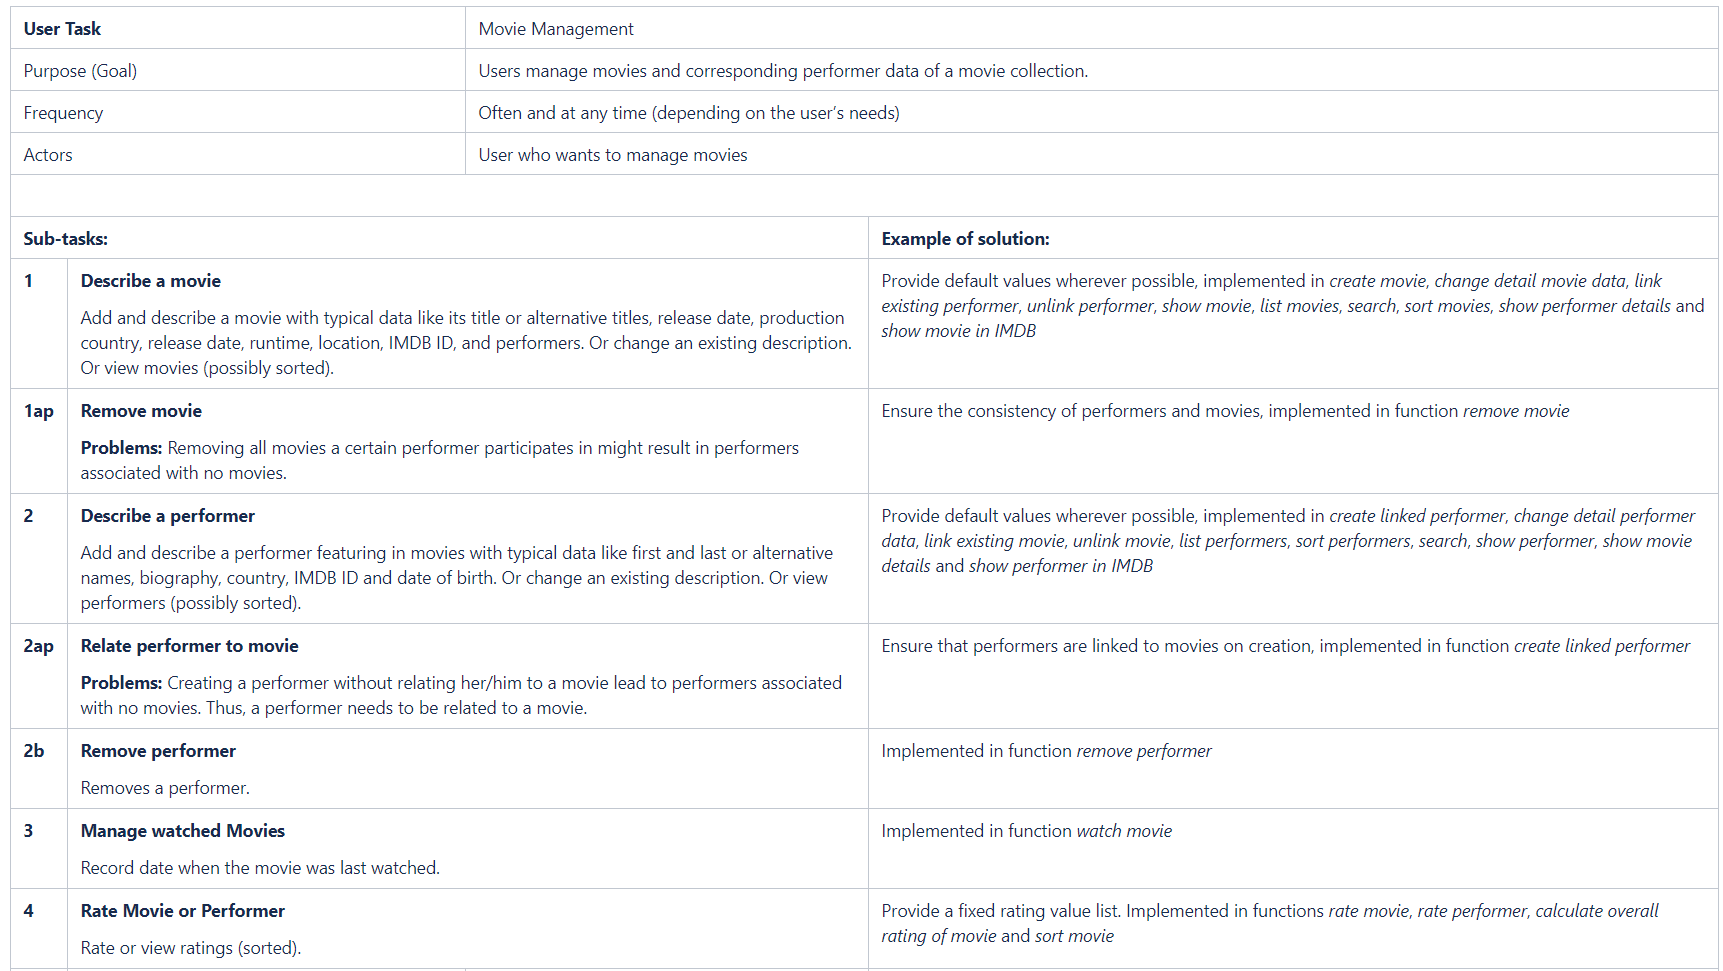
\includegraphics[scale=0.57]{../images/MovieManager.png} 
	\caption{Requirements in User-Task notation for the MovieManager software, an application for managing movie collections.}
	\label{fig:mm}
\end{figure}

\end{landscape}
\restoregeometry



%\chapter{Testing with natural language processing}\label{sec:topic_1}
% Hat aufgehört
%\chapter{Acceptance testing with FitNesse}

% Hickl

\chapter{Systematic Generation of acceptance tests that are executable with FitNesse}
\label{sec:topic_2}

\section{Introduction}\label{sec:topic_2_intro}

This chapter focusses on the creation of acceptance tests that are automatically executable using the tool \textit{FitNesse}.
In this first section of the chapter the reason for using this approach is discussed.
Furthermore, the general features of \textit{FitNesse} as well as the needed artefacts like Fit-tables are explained.
An article that focuses on the topic of creating acceptance tests that are executable with \textit{FitNesse} was provided by the supervisors of the seminar.
Section \ref{sec:literature-search} documents the literature search used to find a different approach.
The two articles are then described in the sections \ref{sec:el-attar} and \ref{sec:longo}.
Moreover, for a better understanding of the presented approaches these chapters include the execution of them on the \textit{MovieManager}.
The following section \ref{sec:comparison} includes the comparison of the two approaches using a synthesis matrix.
Section \ref{sec:topic_2_conclusion} provides a Conclusion including the most important insights of the process and an assessment in which situations the approaches might be suitable.

During the software engineering process communication between the developers and the customers is a crucial factor for the success of the product.
A problem for the communication is the different use of documents by the two main stakeholders:
Customers describe their requirements in natural language whereas the developers create code.
Natural language can often be interpreted in different ways, which can lead to unwanted results.
And whereas code is more precise, it is often too technical for the customer.
Therefore, artefacts are needed that are more precise than natural language and can easily be transformed into code.

One such artefact is a \textit{Fit-table}. 
These tables store easily readable information about acceptance test cases and can be fully automatically executed using the testing tool \textit{FitNesse} \cite{fitnesse}.
Creating \textit{Fit-tables} before the development of the software can help the developers to understand the requirements of the customer by implementing the necessary functionality to pass the acceptance tests.
Thus the customers receive a software that satisfies all their mentioned requirements.
\textit{FitNesse} supports the creation and maintenance of \textit{Fit-tables} as well as the automated execution of the tests represented by the tables.
To make this possible \textit{Fixture-Classes} are needed.
These classes connect the input values from the \textit{Fit-tables} to the \textit{System-under-test} and are executed by \textit{FitNesse}.
An overview of the data exchange during the process is shown in figure \ref{fig:overview-fitnesse} on the next page.
The specific steps are explained in the following:

After the user chooses to execute a set of Fit-tables in \textit{FitNesse}, \textit{FitNesse} executes the Fixture-Classes that belong to the selected tables.
These tables can contain two types of values: Input values and expected output values.
The \textit{Fixture-Class} creates an instance of the \textit{System-under-test} and then transfers the input values into it.
Then it extracts the resulting output values from the \textit{System-under-test} and returns them to \textit{FitNesse}.
These extracted output values are then automatically compared by \textit{FitNesse} to the expected output values from the Fit-tables.
If they are the same, the test was successful and the entry of the table receives the colour \textit{Green}.
Otherwise, the affected part of the test failed and the entry receives the colour \textit{Red}.

\begin{figure}[H]
	\centering
	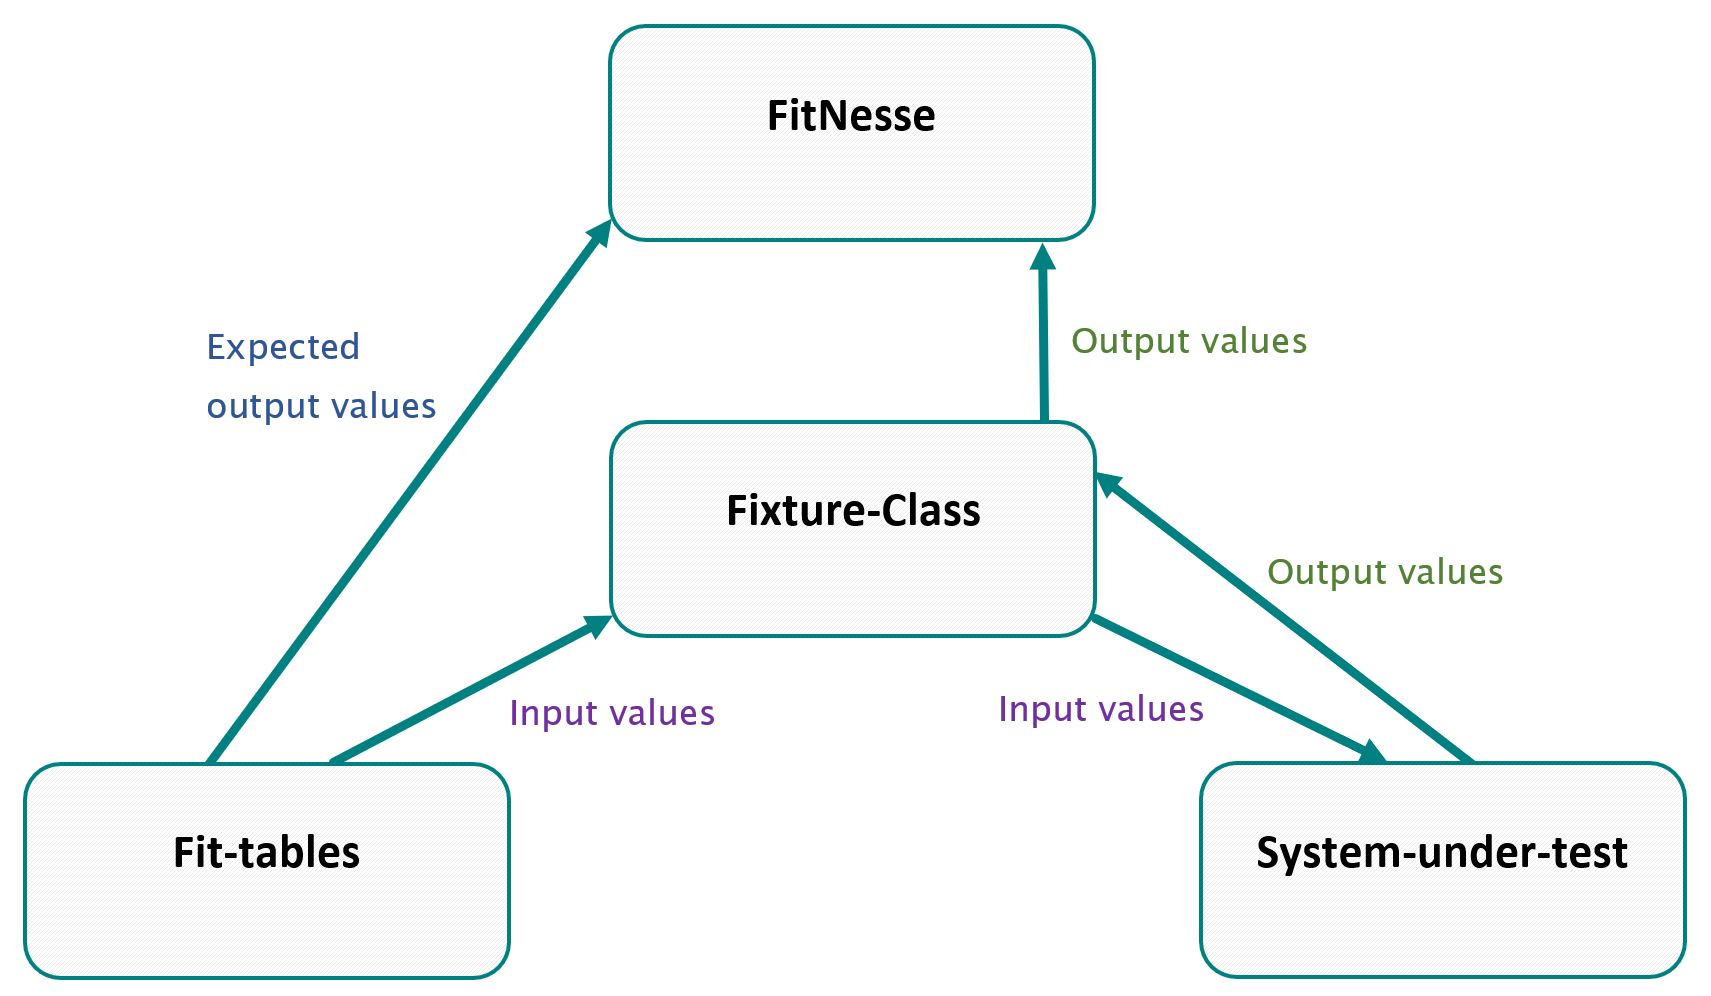
\includegraphics[width=.75\textwidth]{../images/fitnesse-overview.png}
	\caption{Overview of the data exchange in the execution of \textit{Fit-tables} with \textit{FitNesse}. The Fit-tables can be created and maintained in FitNesse.}
	\label{fig:overview-fitnesse}
\end{figure}


\section{Literature search}
\label{sec:literature-search}

The literature search consisted of a search-term-based search as well as forward- and backward-snowballing.
As start article the work of El-Attar and Smith \cite{el-attar} was given by the supervisor of this seminar.
This article presents an approach to create acceptance tests that can be automatically executed using \textit{FitNesse}.
To find more and possibly different approaches the search question was chosen to be:

\begin{center}
\textit{
 Which approaches to systematically generate acceptance tests that are executable with \textit{FitNesse} exist in the literature?
}
\end{center}

\textit{ACM Digital Library} \cite{acm}, \textit{IEEE Xplore} \cite{ieee}, \textit{Springer Link} \cite{springer} and \textit{Science Direct} \cite{elsevier} were used as search platforms as they are the most common platforms in the field of computer science.
The relevance criteria were chosen as follows:
\begin{itemize}
	\item \textit{Criterion 1:} The article describes an approach to systematically generate acceptance tests that are executable with \textit{FitNesse} \textit{or} gives an overview on the use of \textit{FitNesse} in software engineering.
	
	This criterion was chosen to find approaches that are specific to the subject of this chapter.
	Articles that give an overview over the use of \textit{FitNesse} were also accepted because of their potential to classify the found approaches.
	
	\item \textit{Criterion 2:} The article was not published before the year 2009 which is the year that the article by El-Attar and Smith was published.
	
	This criterion was chosen to get a more recent approach than the start article which was by the creation of this chapter already more than 10 years old.
\end{itemize}

Table \ref{fig:lit-search-fitnesse} on the next page provides an overview for the search-term-based literature search.
As search terms the terms \enquote{acceptance test} and \enquote{FitNesse} were chosen.
These search terms turned out to be specific enough to fit only a manageable amount of articles.
The search resulted in eight relevant articles of which six presented an approach and two gave an overview over the use of \textit{FitNesse}.
Both snowballing searches from the start articles did not result in any more relevant articles that were not already found by the search-term-based search.
The backward-snowballing did not result in any relevant articles due to their publishing date and hence not passing Criterion 2.
One relevant article was found during the forward-snowballing that was already found by the search-term-based search on the platform Springer Link.

\begin{table}[H]
	\caption{Overview of the search-term-based literature search.}
	
	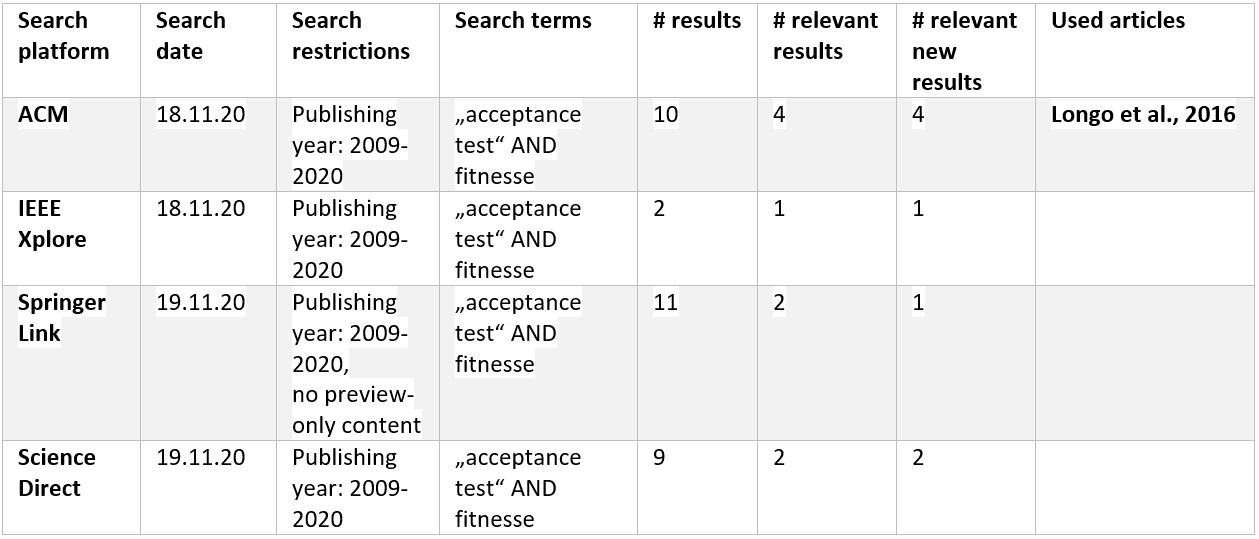
\includegraphics[width=\textwidth]{../images/LitSearchFitnesse.png} 
	
	\label{fig:lit-search-fitnesse}
\end{table}


The articles that gave an overview over the use of FitNesse were not specific about any approaches and only provided general information.
Therefore, none of these articles was used.
As a second approach to compare to the start article, the work by Longo et al. \cite{longo} was chosen.
This article also describes an approach to create acceptance tests that can be automatically executed by \textit{FitNesse}.
The presented approach differs from the approach of the article by El-Attar and Smith in its use of artefacts.
Also it was created by different authors and was published in 2016, so it is a much more recent approach.


\section{Approach 1: Developing comprehensive acceptance tests from Use Cases and robustness diagrams}
\label{sec:el-attar}

\subsection{Description}

El-Attar and Smith \cite{el-attar} introduce an approach to create acceptance tests that can be automatically executed using \textit{FitNesse.}
Their approach is targeted at larger software projects that use a model-based approach such as the use of UML models. 
It was created such that a non-technical person (e.g. a Business Analyst) can execute it during the early phases of the development of the software.
This makes it possible for the developers to follow the approach of Acceptance-Test-Driven-Development (ATDD) because of the possibility of executing the acceptance tests at any time during the development process.
ATDD helps the developers during the development process to evaluate which requirements are already implemented and  which are yet to be implemented.

The approach starts with use case models and domain models as initial artefacts.
During the whole process of creating the acceptance tests every step is performed completely manually.
The execution of the final acceptance tests is done fully automatically by the tool \textit{FitNesse}.
To help with traceability during the approach the authors created a tool called UCAT.
This tool does not provide any automation support but allows the user to create use case models and \textit{Fit-tables}.
These artefacts can be linked within UCAT which helps to determine which use cases resulted in which acceptance tests.
Figure \ref{fig:overview-el-attar} shows the rough structure of the approach.
The exact steps of the approach are described in the following:

\begin{figure}
	\centering
	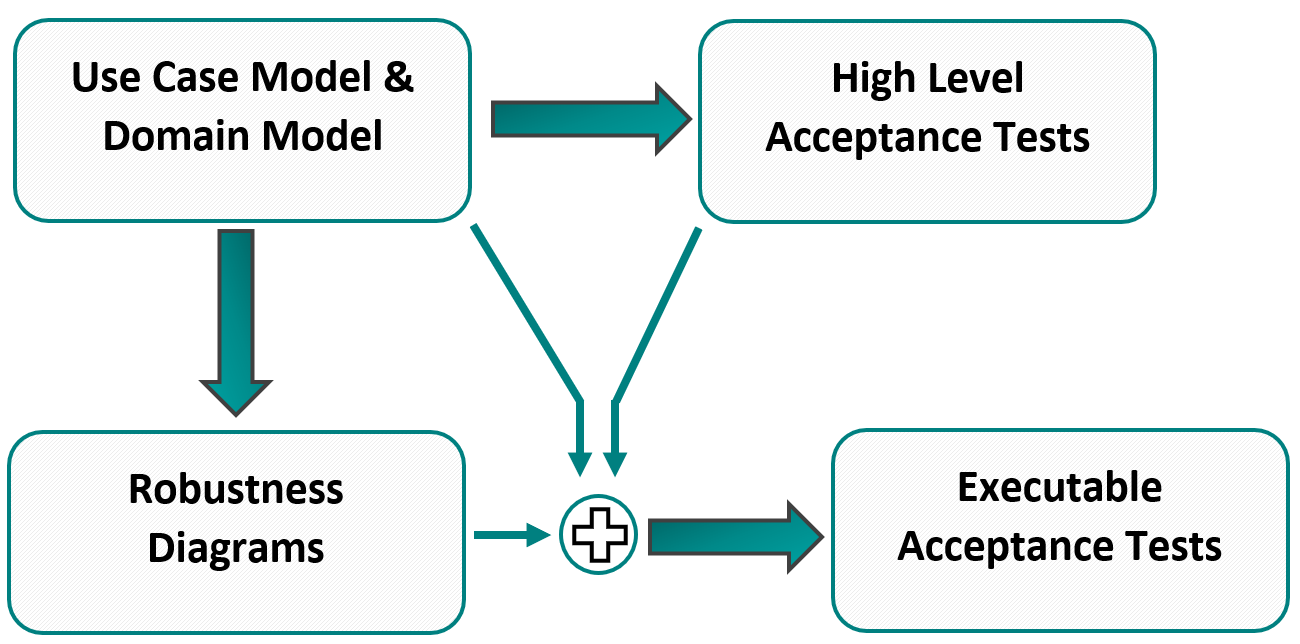
\includegraphics[width=.8\textwidth]{../images/ElAttarProcess.png}
	\caption{Overview of the steps in the approach of El-Attar and Smith.}
	\label{fig:overview-el-attar}
\end{figure}

In the first step of the approach \textbf{High-Level-Acceptance-Tests (HLATs)} are created.
For this a domain model and a Use Case model with Use case descriptions is required in the approach.
HLATs are more informal than an executable acceptance test which helps the analyst to be as flexible as possible in describing the acceptance tests at this early stage.
Commonly Use Cases contain Use Case descriptions from which the flows of the Use Case can be extracted.
HLATs describe the system's expected behaviour during all of the flows of the use cases from the Use Case model.
Necessary Pre-Conditions and triggers for the flows are also extracted from the Use Case description while the inputs for the flows can be extracted from the domain model.
Expected test results are also denoted in the HLATs.
At this point they do not need to contain specific values and can be written in natural language.
The general structure of a HLAT is shown in Table 1.2.


\begin{table}[H]
	\begin{small}
	\caption{General structure of a HLAT.}
	\renewcommand{\arraystretch}{1.5}
	\begin{tabularx}{\textwidth}{X|X|X}
		\hline
  		\textbf{Test ID} & \textbf{Description} & \textbf{Expected \newline Result} \\
  		\hline
  		Name of the Use Case \& the flow & Preconditions: \newline Inputs: & Expected result in natural language \\
  		\hline
 	\end{tabularx}
 	\renewcommand{\arraystretch}{1}
 	\label{fig:1}
 	\end{small}	
\end{table}


After the creation of the HLATs a robustness analysis is performed.
To achieve this, for every use case a \textbf{robustness diagram} is created.
These diagrams combine the use cases from the use case model with the objects from the domain model.
They contain actors and entities as well as boundary- and control-objects.
For each use case all involved objects and the connections between the objects are displayed.
The involved objects and the communication between them is extracted from the Use Case description.
During the creation of the robustness diagrams necessary \textit{objects} or \textit{attributes of objects} may be identified that are not already part of the domain model.
These should be added to the domain model.
Also missing steps or preconditions in the Use Case description might be found.
If this is the case, the Use Case descriptions should also be updated.
After this step the HLATs should be adapted to fit the updated domain model and Use Case descriptions.

In the last step all the existing artefacts (possibly except the domain models) are used to create the final product of the approach: \textbf{Executable Acceptance Tests (EATs)}.
These acceptance tests are in the form of specific \textit{Fit-tables}.
To achieve this, the HLATs have to be divided into smaller steps using the information about the Usage Scenario from the related use case description.
This step requires human judgment and is not further described.
For each of these steps the control flow in the robustness diagram gets traced.
In this process the objects and attributes of each step's input, preconditions, outputs and postconditions are determined.
These where before stated in natural language in the HLAT and are exchanged in the EAT with more concrete objects and attributes.
The steps combined with the corresponding control flow are manually converted into \textit{Fit-tables}.
\textit{Fit-tables} used in this approach are either \textit{ActionFixtures}, \textit{RowFixtures} or \textit{ColumnFixtures} \cite{Fit-tables}.
These types of \textit{Fit-tables} can be fully automatically executed using the tool \textit{FitNesse}.
The domain models are ideally not required if the steps before where executed properly because the information from the domain models should already be part of the use case descriptions.

Due to the fact that the approach of creating the acceptance tests is done completely manually, the quality of the resulting acceptance tests depends highly on the experience and skills of the person executing the approach.
Therefore, the authors state that an evaluation would be beyond the limitations of their work.
However, they provide a case example by applying the approach to the software \textit{RestoMapper}.
This example is not part of this work because in the following section the execution of the approach is presented with the application \textit{Movie Manager} that is used throughout this whole report.

\subsection{Application}

The approach starts with Use Case and Domain Models.
As those are not already described in this article, they are created for this chapter.
Figure \ref{fig:use-case-mm} on the next page shows the Use Case Model for the Movie Manager application.
It contains the use cases and shows connections between them.
For example, removing a movie might result in removing a performer if one of the performers that participated in the movie has no movies anymore after the removal.
Such a relation is highlighted in the Use Case Model with the keyword \textit{extend}.
The domain model of the Movie Manager application is shown in Figure \ref{fig:domain-mm} on the next page.
It contains the entities Movie and Performer as well as the two views that the user can see.

To illustrate the approach the Use Case \textit{Describe a performer} is used.
In the first step of the approach the HLATs for this Use Case need to be created.
The User Scenarios for this Use Case are as mentioned in the User Task table:
\begin{itemize}
	\item Add and describe a performer
	\item Change the description of an existing performer
	\item View performers (possibly sorted)
\end{itemize}

\begin{figure}[H]
	\centering
	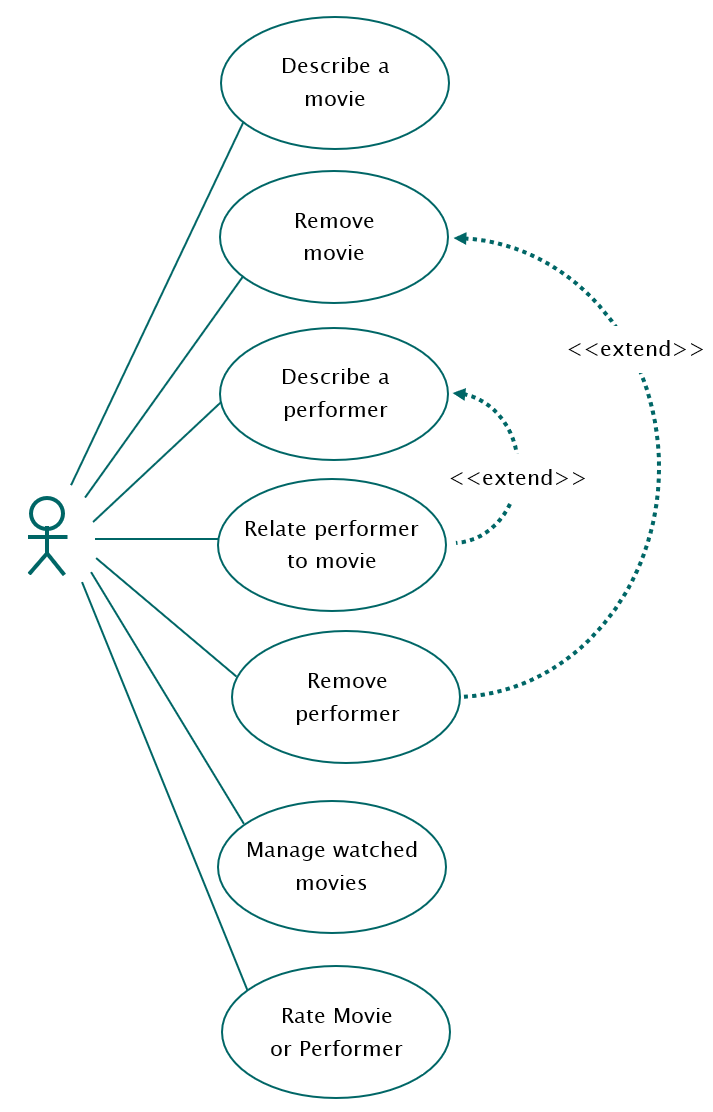
\includegraphics[width=.5\textwidth]{../images/ElAttarUseCase.png}
	\caption{Use Case Model for the Movie Manager application.}
	\label{fig:use-case-mm}
\end{figure}



\begin{figure}[H]
	\centering
	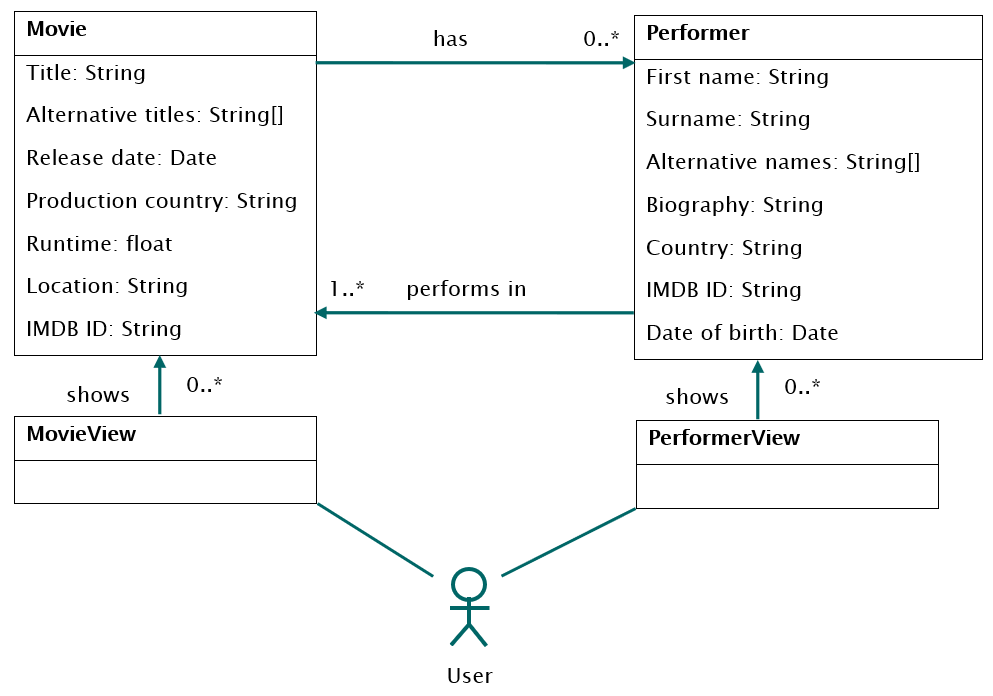
\includegraphics[width=.8\textwidth]{../images/ElAttarDomain.png}
	\caption{Domain Model for the Movie Manager application.}
	\label{fig:domain-mm}
\end{figure}



The HLATs for the Use Case \textit{Describe a Performer} are displayed in Table \ref{fig:hlats-mm}.
Each HLAT describes the necessary preconditions, inputs and the expected results of one User Scenario.
This information is extracted from Use Case description.

\begin{table}[H]
	\caption{HLATs for the Use Case \textit{Describe a performer} of the Movie Manager application.}	
	\centering
	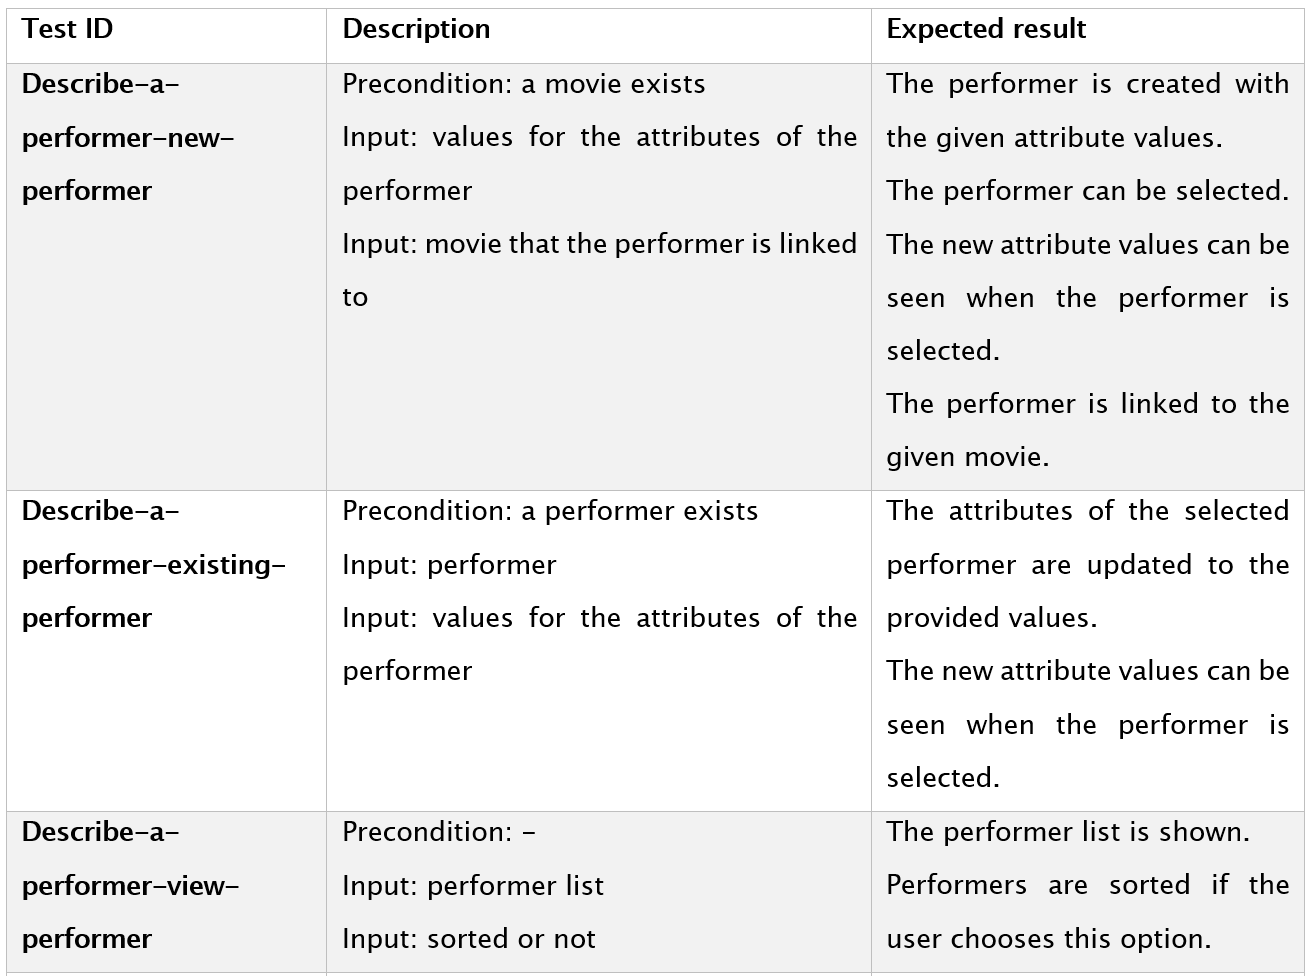
\includegraphics[width=.9\textwidth]{../images/ElAttarHLATs.png}
	\label{fig:hlats-mm}
\end{table}

In the next step a robustness diagram is created using the information from the Use Case Model and the Domain Model.
The robustness diagram for the Use Case \textit{Describe a movie} is shown in figure \ref{fig:robustness-mm} on the next page.
A robustness diagram contains the involved objects that communicate with the user.
These are called boundary objects.
An example for a boundary object is \textit{PerformerView} in figure \ref{fig:robustness-mm}.
It also contains control-objects like \textit{RelateToMovie} in figure \ref{fig:robustness-mm} that makes sure that a performer is related to at least one movie.
The last types of objects are the \textit{User} and the entities like \textit{Performer} or \textit{Movie} in figure \ref{fig:robustness-mm}.
The resulting robustness diagram is used to find new information for the domain diagram.
For example, CheckMovieRelations needs to find out whether the performer is linked to at least one existing movie.
Therefore, the domain model needs to include a list of related movies for each performer or the number of related movies.
In this example the first variant (a list of related movies) is used in the domain model.
So this specific information does not have to be added.
Overall the robustness analysis does not bring up any new information but possibly could for other examples which is why El-Attar and Smith have included it in their approach.


\begin{figure}[h!]
	\centering
	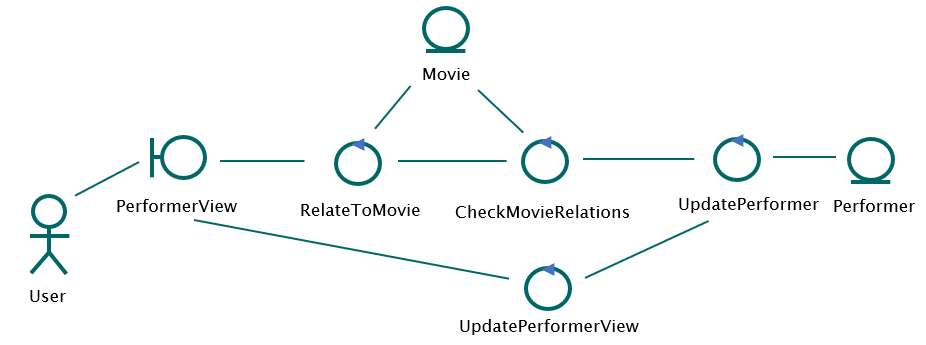
\includegraphics[width=.8\textwidth]{../images/ElAttarRobustness.png}
	\caption{Robustness Diagram for the Use Case \textit{Describe a performer} of the Movie Manager application.}
	\label{fig:robustness-mm}
\end{figure}



As last step executable acceptance tests are created for each HLAT.
These are created in the form of \textit{Fit-tables}.
For this example so called \textit{ActionFixtures} are chosen but \textit{RowFixtures} and \textit{ColumnFixtures} are also possible for this approach.
\textit{ActionFixtures} contain a Test ID in the first row.
Each of the following rows contains one action like entering a value or pressing a button.
The ActionFixtures for the three HLATs from table \ref{fig:hlats-mm} are displayed in the tables \ref{fig:eats1-mm}, \ref{fig:eats2-mm} and \ref{fig:eats3-mm} on the next page.
These Fit-tables are the final result of the approach.

\begin{table}[H]
	\caption{Executable Acceptance Tests for the scenario \textit{Describe a performer, new performer} of the Movie Manager application in form of an \textit{ActionFixture}. 
	A placeholder in the form of \textit{...} is used for entering the other possible attributes of a performer to reduce the size of the table.}
	\centering
	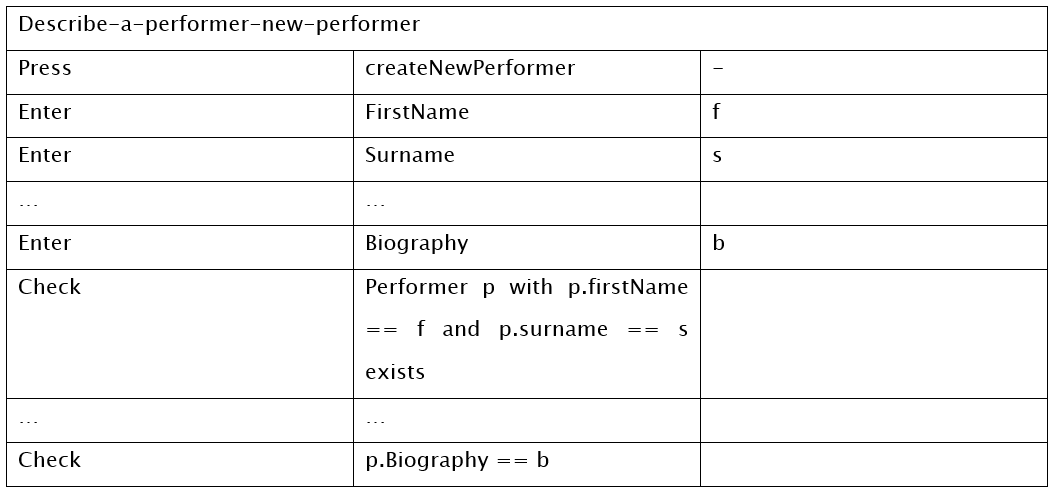
\includegraphics[width=.9\textwidth]{../images/ElAttarEATs1.png}
	\label{fig:eats1-mm}
\end{table}

\begin{table}[H]
	\caption{Executable Acceptance Tests for the scenario \textit{Describe a performer, existing performer} of the Movie Manager application in form of an \textit{ActionFixture}.
	A placeholder in the form of \textit{...} is used for entering the other possible attributes of a performer to reduce the size of the table.}
	\centering
	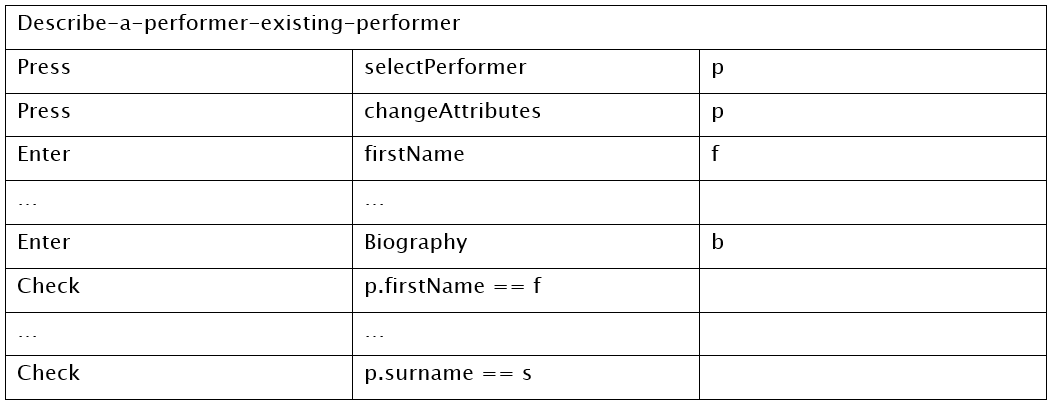
\includegraphics[width=.9\textwidth]{../images/ElAttarEATs2.png}	
	\label{fig:eats2-mm}
\end{table}

\begin{table}[H]
	\caption{Executable Acceptance Tests for the scenario \textit{Describe a performer, view performers} of the Movie Manager application in form of an \textit{ActionFixture}.
	A placeholder in the form of \textit{...} is used for entering the other possible attributes of a performer to reduce the size of the table.}
	\centering
	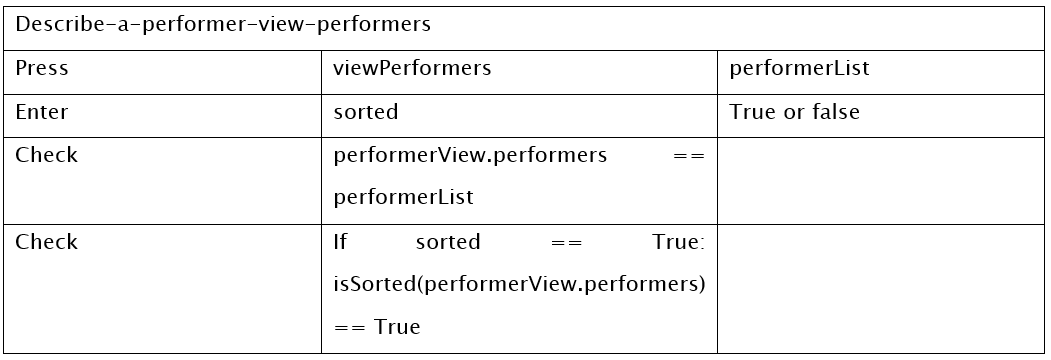
\includegraphics[width=.9\textwidth]{../images/ElAttarEATs3.png}
	\label{fig:eats3-mm}
\end{table}


\section{Approach 2: A web framework for test automation, user scenarios through user interaction diagrams}
\label{sec:longo}

\subsection{Description}

Longo et al. \cite{longo} create User Scenarios through User Interaction Diagrams (US-UIDs) which then are fully automatically converted into \textit{Fit-tables} that represent the test data for acceptance tests.
To run these acceptance tests a Fixture-Class is needed that connects the test data from the \textit{Fit-table} with the System-under-test.
The US-UIDs are created in a tool provided by the authors.
They contain functional data such as the involved objects, attributes and functions and also explicit User Scenarios provided by the customer.
The User Scenarios provide the test data and combined with the functional data, \textit{Fit-tables} can be automatically created.
The functional data represents the top row of the \textit{Fit-table} and the User Scenarios the specific values.
Figure \ref{fig:overview-longo} provides an overview over the steps of the approach.
The only step that is executed automatically is marked in this overview.
Each of the steps is explained in more detail in the following.

\begin{figure}[H]
	\centering
	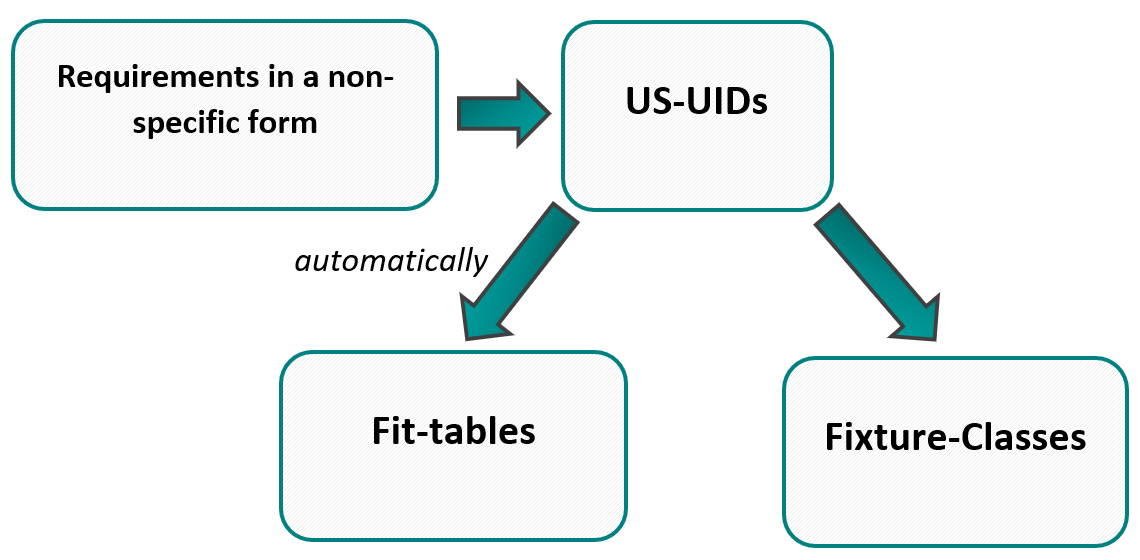
\includegraphics[width=.62\textwidth]{../images/LongoProcess.png}
	\caption{Overview of the steps in the approach of Longo et al.}
	\label{fig:overview-longo}
\end{figure}
\newpage
In the first step the US-UIDs are created.
This step is described in another work by the authors \cite{longo2}.
Each US-UID contains an explicit User Scenario provided by the customer.
The information about the User Scenario is extended by the developer by adding functional information.
For example, the User Scenario could provide a specific value for a variable.
Then the functional information for this value would be the name of the variable.
With this conjunction of explicit and functional values \textit{Fit-tables} can be automatically created.
The first row contains the functional information.
Each row after the first row represents a User Scenario and contains the given values for the functional information (objects, variables, etc.) given in the first row.

Each row can be used as one specific test case.
To execute these test cases a Fixture-Class is needed.
This class has to be written by the developers.
It creates an instance of the System-under-test and uses \textit{Setter methods} to provide the input from the \textit{Fit-table} to the System-under-test.
Through \textit{Getter methods} the resulting values of the System-under-test can be extracted to validate the success of the test.
For the evaluation step the results from the Getter methods are compared to the expected values from the \textit{Fit-table}.
If they are the same, the test was successful.

To evaluate their approach Longo et al. used their tool to automatically create executable acceptance tests from existing US-UIDs.
The developers of the software related to these US-UIDs already manually created test cases for the software.
In the evaluation the authors compared these manually created tests to the tests created by their tool.
To compare both of them the authors used the techniques \textit{code mutation} and \textit{lack of code}.
The technique \textit{code mutation} involved manipulating the values of an array in the software and \textit{lack of code} was executed by removing a class from the software.
By using both techniques failed tests could be found in both test sets.
The second technique also resulted for both test sets in tests that were not executable.
From these results the authors concluded that tests created with their approach can detect test cases that are \textit{successful}, \textit{failed} or \textit{not executable}.

\subsection{Application}

To illustrate the approach of Longo et al. the use case \textit{Describe a performer (new performer)} is used.
In the first step an US-UID has to be created that displays the explicit information of a User Scenario as well as the underlying functional information.
In this type of model the round boxes are states of the system.
The rectangles contain the User's Input whilst the free text in the round boxes describes the system's output.
Arrows are used to assign functional names to the data and to denote transitions between states.
The US-UID for the example is displayed in figure \ref{fig:us-uid-mm}.
In the beginning the performerList contains only the performers a, b and c with attributes e, f and g.
After the execution of the US-UID it also contains performer d with attributes x.


\begin{figure}[tbh]
	\centering
	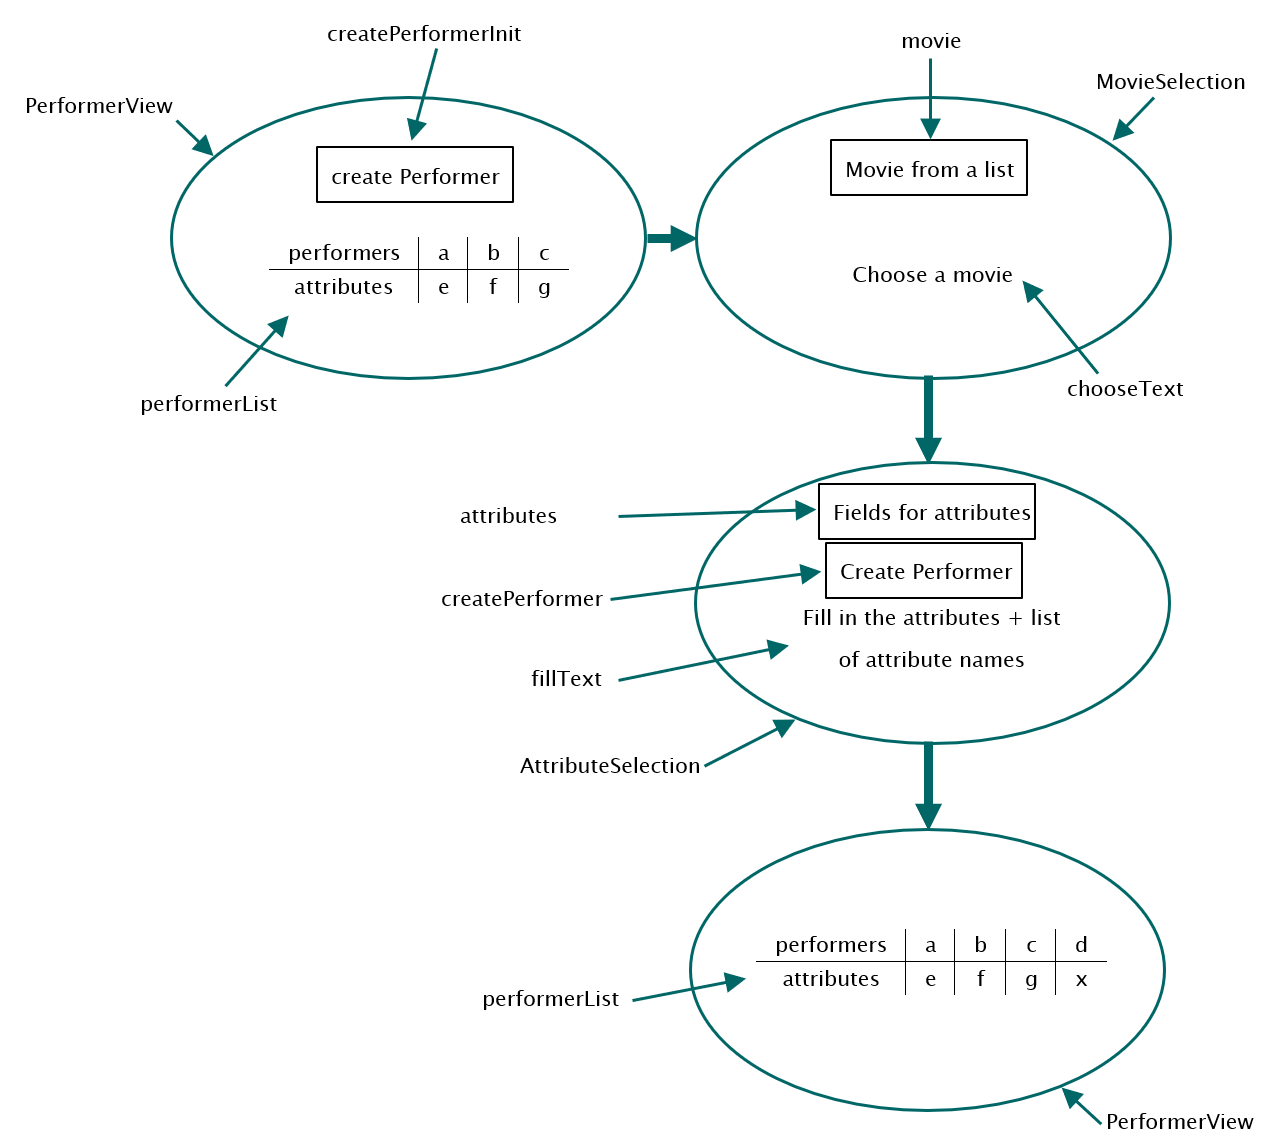
\includegraphics[width=.85\textwidth]{../images/US-UID.png}
	\caption{US-UID for the Use Case \textit{Describe a performer (new performer)} of the Movie Manager application.}
	\label{fig:us-uid-mm}
\end{figure}

In the next step the functional information from the US-UID needs to be connected to the real
objects and attributes of the \textit{System-under-test}. This is done in a Fixture-Class that is marked
with \textit{@Fixture}.
This class has to be written manually.
The data flow during the execution of acceptance tests with FitNesse and the role of the Fixture-Class in this process is described in section \ref{sec:topic_2_intro}.
Inputs are part of the functional data on the start of the arrows in the US-UIDs. 
For the first display of the US-UID PerformerView the Fixture-Class needs methods to move to the next display, to set the starting performer list and to choose
\textit{create Performer}.
Results have to be extracted from the System-under-test using Getter-Methods.
One such result is the updated performer list in the last state of the PerformerView.
This result can be compared to the expected result given in the US-UID.

In the final step a \textit{Fit-Table} is created.
This step is fully automatic with the tool of Longo et al. because it is only remodeling information from the US-UID.
The functional information is placed in the top row whilst the explicit data of the User Scenarios is stored in the following rows.
Each row represents an User Scenario.
The resulting \textit{Fit-table} for the example is displayed in table \ref{fig:fit-longo} on the next page.

\begin{table}[h!]
	\caption{\textit{Fit-table} for a specific User Scenario of the Use Case \textit{Describe a performer (new performer)} of the Movie Manager application. The expected results end with a question mark.}
	\centering
	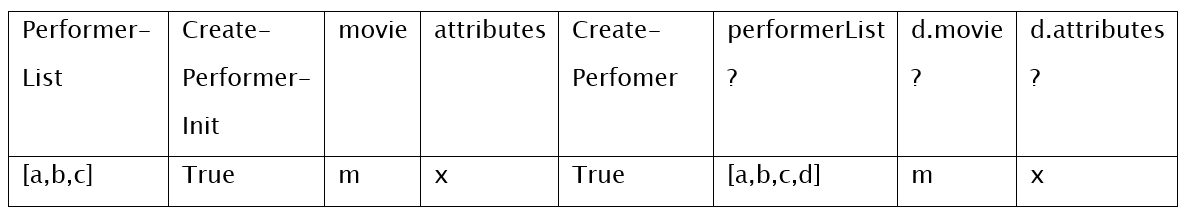
\includegraphics[width=\textwidth]{../images/LongoFit.png}

	
	\label{fig:fit-longo}
\end{table}

\newpage
\section{Comparison}
\label{sec:comparison}

As in the other chapters the approaches are compared in a synthesis matrix.

\renewcommand{\arraystretch}{1.5}
%	\begin{tabularx}{\textwidth}{>{\hsize=.2\hsize}X X}
%  		\textbf{1a} & Which artefacts and relations between artefacts are used in this approach? Which
%artefacts are created in the course of the approach? How are the artefacts characterized?
% \\
%  		\hline
%  		\textbf{1b} & What is required and/or input for the application of the approach? \\
%  		\hline
%  		\textbf{1c} & What steps does the approach consist of? Which information is used in which step
%and how? What are the results of the individual steps?
% \\
%  		\hline
%  		\textbf{2a} & Which usage scenarios are supported by the approach? \\
%  		\hline
%  		\textbf{2b} & Which stakeholders are supported by the usage scenarios? \\
%  		\hline
%  		\textbf{2c} &  Which knowledge areas from SWEBOK can be assigned to the usage scenarios? \\
%  		\hline
%  		\textbf{3a} & What tool support is provided for the approach? \\
%  		\hline
%  		\textbf{3b} & Which steps of the approach are automated by a tool? Which steps are supported
%by a tool, but still have to be executed manually? Which steps are not supported
%by a tool?
% \\
%  		\hline
%  		\textbf{4a} & How was the approach evaluated? \\
%  		\hline
%  		\textbf{4b} & What are the (main) results of the evaluation? \\
%  		\end{tabularx}
 
\begin{small} 		
\begin{longtable}[h]{p{0.45cm}|p{0.425\textwidth}|p{0.425\textwidth}}
	\caption{Synthesis matrix}
	\label{tab:blub}
	\\    %%%%<===
	\hline
  	\textbf{Nr.} & \textbf{Approach 1} & \textbf{Approach 2}\\
  	\hline
  		 1a) & Initial artefacts: \textbf{Use Case and Domain Models} are used to create high level acceptance tests and robustness diagrams 
\textbf{Robustness diagrams} combine the information from the use cases and the domain model. During the creation of the robustness diagrams for the use cases objects and attributes may be identified that are missing in the domain model. The domain model is updated with this missing information.
\textbf{High level acceptance tests (HLATs)} deliver an informal description of acceptance tests. They are tables and use keywords that are chosen by their creator. For each flow of a use case from the Use Case model a HLAT is created.
\textbf{Fit-tables} are a form of executable acceptance tests that can be automatically executed by the tool FitNesse. For each HLAT a Fit-table is created using the information about the control flow in the respective robustness diagram.
 & \textbf{User Scenarios through User Interaction Diagrams (US-UIDs)} show the interaction during a User Scenario. They include User-Input, System-Output, states of interaction and transitions between states.
\textbf{Fit-tables} are a form of executable acceptance tests that can be automatically executed by the tool FitNesse. The Fit-tables in this approach need a specific Fixture-Class for each Use Case that allows the flow of information between the Fit-table and the System-under-test.
 \\
 \hline
  1b) & \begin{itemize}
  		 \item Use Case Model \item Domain Model
\end{itemize}  		  & Requirements in a non-specific type \\
	\hline
  1c) & As initial artefacts Use Case models and Domain models are used.
In the first step a HLAT is created for each flow of each use case from the Use Case model. The information about the preconditions, inputs and triggers for the HLATs gets extracted from the domain model.
The second step is the creation of robustness diagrams for the use cases from the Use Case model. These diagrams also include the objects from the domain model and model the communication between those in the specific use case. If objects or attributes are found in this step that are necessary but not yet part of the domain model, they are added to the domain model. All the other models are updated to fit the domain model. In the last step a Fit-table is created for each HLAT using the control flow that can be seen in the robustness diagram. 
Finally the created Fit-tables can be combined with the Use Case from the Use Case model that they belong to.
 & In the first step the US-UIDs are created by using the known requirements.
The customer delivers the User Scenario and the developer add the functional information for the data used in the scenario.
The Fit-tables are created automatically from the information of the US-UIDs. This step is done by the web framework.\\
\hline
  2a) & Business Analysts receive a systematic approach to create acceptance tests in the Fit-syntax.
Customers receive a product that fits their requirements.
Developers receive acceptance tests that they can use to determine which requirements of the customers they have already implemented and which they have to work on.
 & Customers and developers receive an approach to develop acceptance tests together that include User scenarios provided by the customer.
Developers receive acceptance tests that they can use to determine which requirements of the customers they have already implemented and which they have to work on.
 \\
  \hline
  		 2b) & 
  		 	\begin{itemize}
  		 		\item Developer 
  		 		\item Customer 
  		 		\item  Business Analyst
			\end{itemize}  		 
			& \begin{itemize}
  		 		\item Developer 
  		 		\item Customer
				\end{itemize}\\
	 \hline
  		 2c) & Developer: Software Construction (Test-driven development) \newline
Business Analyst \& Customer: Software Testing
 & Customer/Developer: Software Requirements, Software Testing \newline
Developer: Software Construction (Test-Driven Development)
 \\
  		\hline
  		 3a) & The authors provide the tool UCAT in which Use Case Models and Fit-tables can be created and linked. The created Fit-tables can be automatically executed using FitNesse. & A web framework is provided by the authors in which US-UIDs can be created and converted to Fit-tables. These Fit-tables can be executed with FitNesse. \\
  	 \hline
  		 3b) & The tool UCAT serves as an editor to create Use Case models and Fit-tables. Those two artefacts can also be linked in UCAT.
Every other step in the creation of the acceptance tests is done without tool support.
No step of the approach is done automatically.
 & The creation of the US-UIDs is supported by the web framework which serves as an editor.
Converting the US-UIDs to Fit-tables is done fully automatically by the web framework.
Every other step in the creation of the acceptance tests is done without tool support.
 \\
  \hline
  4a) & 
  	\begin{itemize} 
  		\item Case study with an application (RestoMapper)
		\item	No real evaluation 
	\end{itemize}
 & The authors created tests automatically from existing US-UIDs of an existing application using their approach.
The resulting test set was compared to an existing test set that was created manually.
The code of the application was manipulated using code mutation and lack of code.
For the method code mutation the values of an array were changed manually. For lack of code a class was deleted.
 \\
  \hline
  		 4b & The approach can be applied on an example.
Otherwise no evaluation results because the authors state that an evaluation is beyond the limitations of their work.
The reason for this is that the quality of the created tests in this approach highly depends on the experience and skill of the person executing the approach.
 & Code mutation and lack of code resulted for both test sets in failed tests.
Lack of code also resulted in not executable tests.
The authors concluded that the tests created by their approach can successfully classify tests as successful, failed or not executable.
 \\
  \hline
\end{longtable}
\end{small}

Both approaches provide a possible way to create acceptance tests that are executable with the tool \textit{FitNesse}.
El-Attar and Smith utilize use case models and domain models as their initial data while Longo et al. only need a non-specific description of the use cases.
Generally El-Attar and Smith use more artefacts as their approach needs use case models, domain models, high-level acceptance tests and robustness diagrams as intermediate steps to the final representation of the executable acceptance tests.
In the approach of Longo et al. only US-UIDs need to be created which are then automatically converted to \textit{Fit-tables}.
In contrary to El-Attar and Smith the approach of Longo et al. requires the creation of some code in the process:
This is the case because the used \textit{Fit-tables} differ between the two approaches.
While El-Attar and Smith use the specific table types ActionFixture, RowFixture and ColumnFixture, Longo et al. use easier \textit{Fit-tables} that are connected to the System-under-test via a Fixture-Class.
This Fixture-Class has to be written manually.

Both approaches provide a tool to combine artefacts with the resulting acceptance tests which helps traceability.
For both approaches the creation of the executable acceptance tests is still mostly or completely manual.
While the approach of El-Attar and Smith uses no automation during the creation of the executable acceptance tests, the last step of the approach of Longo et al. is fully automatically.
This is possible because the US-UIDs created in the approach of Longo et al. are a different way to display the information of a \textit{Fit-table} and therefore can be directly converted to a \textit{Fit-table}.
The execution of the final acceptance tests is fully automatic for both approaches.

Both approaches involve customer and developers as stakeholders.
The customer delivers the User Scenarios and receives (because of the development of acceptance tests) potentially a final product that is closer to his needs.
The developers receive automatically executable tests that help them during the development process to determine which requirements are already satisfied and which still need to be implemented.
While in the approach of Longo et al. the creation process of the acceptance tests is done by the customer and the developers together, in the approach of El-Attar and Smith a Business Analyst is responsible for this process.

El-Attar and Smith only visualize their approach through an example and state that the approach cannot be validated in their work because it is beyond the limitations of their work.
The reason for this is that all the steps to create the acceptance tests are done manually and therefore depend on the experience and skill of the analyst performing the steps.
Longo et al. include a small evaluation in their work.
They compare the tests created by their approach to tests that are created without guidelines from the same US-UIDs.
During the testing phase they conclude that the tests created by their approach can be classified as \textit{successful}, \textit{failed} or \textit{not executable}.
Also changes in the source code of the System-under-test resulted in failed tests for both of the test sets which leads the authors to the conclusion that both the tests created without guidelines as well as the tests created with their approach can detect fails in the System-under-test.


\section{Conclusion}
\label{sec:topic_2_conclusion}

The literature search showed that creating acceptance tests that are automatically executable with the specific tool \textit{FitNesse} is not a widely researched topic in the literature.
However, approaches exist that differ in their process to create tests.
Two of these approaches were presented in this chapter:

The approach by El-Attar \& Smith is aimed at larger projects and therefore, might not be useful for smaller products.
It requires the creation of a lot of UML models.
If an analyst exists that has experience in creating these models and at least a few of the used models are created anyway in the engineering process, then this approach might be useful.

The second approach by Longo et al. could be used for smaller projects where the customer is heavily involved.
The customers have to be involved because they have to provide the User Scenarios in this approach.
The approach is heavily dependent on the creation of US-UIDs that contain the information of Fit-tables in a different (possibly better) way.
If the developers and customers prefer US-UIDs over Fit-tables and they want to use User Scenarios, this approach might be useful.

Overall, in the considered approaches the creation of acceptance tests is a process that is highly dependent on the experience and skill of the persons involved.
Once the executable tests are created they are an easy way to measure how well the requirements of the customer are implemented.


\chapter{Testing with a transition system}\label{sec:topic_3}

\section{Introduction}

System tests are used to make sure that clients receive exactly the kind of software they previously specified within the order contract submitted to the software vendor. Oftentimes what was specified and what was implemented does not match entirely in the end. The software vendor faces traceability problems to track which requirements could be covered in which tests and therefore which requirements got implemented. How does one make sure that each atomic functional and robustness requirement specified is covered in the requirements' implementation?

To solve this, the process of formal definition of requirements and matching system tests must be brought closer together. Testing should already be possible in early stages of development, to be precise during the specification phase already. To automatically derive test scenarios from means of the specification area \textit{transition systems} are used. They help to generate test paths as possible combinations of fine-grained functional requirements received through the traversal. An equivalent approach can be used to derive robustness tests as well. In this process requirements can furthermore be tested on their consistency, correctness and integration and eventually can be refined further.

For this purpose the two approaches \cite{ClementineNebut2006} and \cite{NajlaRaza2007} were analyzed. While \cite{ClementineNebut2006} was given in advance by the advisors, \cite{NajlaRaza2007} was discovered through an extensive literature search shown in \autoref{literaturesearch}. Both approaches will be explained in the following sections \autoref{approachone} and \autoref{approachtwo} and applied to the movie management software example. A comparison between the two approaches will be drawn using a synthesis matrix shown in \autoref{comparison}. The main results of testing with transitions systems will be summarized in \autoref{conclusion}. 

Please refer to the glossary in order to receive a common understanding of the following terms used in the sections below: contract, coverage criterion, interaction overview diagram, object constraint language, operation, test case, test objective, test scenario, transition system, UC-System, UC-SCSystem, use case, use case scenario, XML metadata interchange.

\section{Literature search} \label{literaturesearch}

The literature research was driven by the central research question (RQ): 

\glqq Which approaches for automatic generation of system tests exist that are using contract enriched use cases or other use case related means of the specification area within a transition system simulation model?\grqq 

The focus during this literature search was on finding a second approach to automatically generate system tests from means of the specification phase by exhaustively simulating a transition system to generate test paths similar to \cite{ClementineNebut2006}. But as \cite{ClementineNebut2006} is restricted on using \textit{contract} enriched \textit{use cases} and \textit{use case scenarios}, the way how \textit{test objectives} are derived was this time freely selectable to receive another new, but similar approach. The pre-search results were promising both on IEEE Xplore and ACM \cite{ieee, acm}. Only some papers on ACM could not be accessed publicly. The number of results was considered to be sufficient to cover all relevant scientific papers, which is why the research was restricted on these two platforms. Furthermore, two relevance criteria inspired by the central RQ were defined:

\begin{itemize}
	\item Does the method described in the article generate system tests automatically from use cases or other use case related means of the specification area?
	\item Are test objectives generated using some kind of simulation model based on use case contracts (pre- and postconditions) or similar transition system approaches?
\end{itemize} 

As system tests can not exclusively be derived from means of the specification area, an article should restrict to generating system tests from use case related means of the specification area. To derive test objectives a transition system should be simulated exhaustively based on contract definitions (pre- and postconditions). 

The search was done using both snowballing and search term techniques. 140 papers were found referencing \cite{ClementineNebut2006} and 46 articles were referenced by \cite{ClementineNebut2006}. The results of the snowballing search can be found in \autoref{snowballing}. The backward snowballing approach was restricted on references stated in the \textit{Related Work} chapter as all other references relate to preceding work that serve as basic knowledge to realize the transition system approach in \cite{ClementineNebut2006}. Additionally, most of the references were quite old since the original paper was published in 2006. Therefore not all papers could be found on IEEE Xplore or ACM, which is why the number of considered papers is even lower than the number of original references found. Why specific papers were considered not suitable or only partly suitable is documented in \cite{FelixHausberger2020}.

\begin{small}
	\begin{longtable}{l|c|c|c}
		\caption{Results of snowballing techniques}
		\label{snowballing}	
		\\    %%%%<===
		\hline
		 & \textbf{Yes} & \textbf{Possibly} & \textbf{No} \\
		\hline	
		Forward snowballing & 5 & 9 & 63 \\
		\hline
		Backward snowballing & 2 & 1 & 2 \\
		\hline
	\end{longtable}
\end{small}


Seach-term based search was done using the following key terms: system tests, automatic generation, transition system, simulation model, use cases, contracts. Only papers published between 2006 and 2020 having the search term \enquote{test} and \enquote{use case} in their publication title were evaluated. 

\newpage


\begin{longtable}[h]{c|c|p{0.2\textwidth}|p{0.2\textwidth}|c}
		\caption{Results of search-term based technique}
		\label{search-term}\setlength{\tabcolsep}{1em}\\
		\hline
		\textbf{Source} & \textbf{Date} & \textbf{Search restrictions} & \textbf{Search query} & \textbf{\#Results} \\
		\hline
		IEEE Xplore & 2020-11-21 & \enquote{system tests} in document title; \enquote{automatic generation} in document title; \enquote{transition system} in full text \& metadata; \enquote{simulation model} in full text \& metadata; \enquote{use cases} in document title; \enquote{contracts} in full text \& metadata; & \enquote{system tests} AND \enquote{automatic generation} AND \enquote{transition system} AND \enquote{simulation model} AND \enquote{use cases} AND contracts & 0 \\
		\hline
		IEEE Xplore & 2020-11-21 & \enquote{system tests} in document title; \enquote{automatic generation} in abstract; \enquote{transition system} in full text \& metadata; \enquote{use cases} in document title; \enquote{contracts} in full text \& metadata; & \enquote{system tests} AND \enquote{automatic generation} AND \enquote{transition system} AND \enquote{use cases} AND contracts & 0 \\
		\hline
		IEEE Xplore & 2020-11-21 & \enquote{test} in document title; \enquote{transition system} in full text \& metadata; \enquote{use cases} in document title & \enquote{system tests} AND \enquote{transition system} AND \enquote{use cases} & 82 \\
		\hline
		ACM & 2020-11-21 & \enquote{system tests} in title; \enquote{automatic generation} in title; \enquote{transition system} in full text; \enquote{simulation model} in full text; \enquote{use cases} in title; \enquote{contracts} in full text; & \enquote{system tests} AND \enquote{automatic generation} AND \enquote{transition system} AND \enquote{simulation model} AND \enquote{use cases} AND contracts & 0 \\
		\hline
		ACM & 2020-11-21 & \enquote{system tests} in title; \enquote{automatic generation} in abstract; \enquote{transition system} in full text; \enquote{use cases} in title; \enquote{contracts} in full text; & \enquote{system tests} AND \enquote{automatic generation} AND \enquote{transition system} AND \enquote{use case} AND contracts & 0 \\
		\hline
		ACM & 2020-11-21 & \enquote{system tests} in title; \enquote{transition system} in full text; \enquote{use cases} in title & \enquote{system tests} AND \enquote{transition system} AND \enquote{use cases} & 0 \\
		\hline
		ACM & 2020-11-21 & \enquote{test} in title; \enquote{use case} in title & \enquote{system tests} AND \enquote{use case} & 8 \\
		\hline
\end{longtable}

From the resulting papers, only one was considered suitable as a potential second paper. After the search for potential articles to be evaluated was finished, a choice between eight remaining papers from the initial search had to be made:

\begin{itemize}
	\item System Testing using UML Models \cite{MonalisaSarma2007},
	\item An Automatic Tool for Generating Test Cases from the System's Requirements \cite{RosziatiIbrahim2007},
	\item Automated Test Case Generation from Use Case: A Model Based Approach \cite{LizheChen2010},
	\item Requirements Document Based Test Scenario Generation for Web Application Scenario Testing \cite{XiaojingZhang2015},
	\item An Approach to Modeling and Testing Web Applications Based on Use Cases \cite{LipingLi2008},
	\item Test cases generation from UML state diagrams \cite{YGKim1999},
	\item Requirements by Contracts allow Automated System Testing \cite{ClementineNebut2003},
	\item An Automated Approach to System Testing Based on Scenarios and Operations Contracts \cite{NajlaRaza2007}.
\end{itemize}

The decision criteria are based on the different search terms mentioned above and the already defined criteria. Additionally, focus of the selected paper should lie on creating system tests for any generic application area, not just UI related parts of an application.

The paper \textit{An Automatic Tool for Generating Test Cases from the System's Requirements} was not chosen as it does not focus on testing the consistency of use case combinations with contracts to build test objectives as in the original paper. Furthermore, it is not as in-depth as the original paper. Contract enriched use cases could neither be found in \textit{System Testing using UML Models}.

\textit{Automated Test Case Generation from Use Case: A Model Based Approach} really embodies the principle of state base modeling based on use cases with its \textit{interaction finite automaton} (IFA), but doesn't introduce a formal language to define use cases and its contracts.

\textit{Requirements Document Based Test Scenario Generation for Web Application Scenario Testing} as well as \textit{An Approach to Modeling and Testing Web Applications Based on Use Cases} are specifically optimized for web application \textit{test scenarios} and therefore not as general and universally applicable as the original paper.

\textit{Test cases generation from UML state diagrams} and \textit{Requirements by Contracts allow Automated System Testing} could unfortunately not be accessed in full length in IEEE Xplore.

The chosen article to further evaluate is \textit{An Automated Approach to System Testing based on Scenarios and Operations Contracts}, as it introduces a second way to create system tests from use case scenarios as UML 2.0 models by enriching it with contracts and by transforming the formalized scenarios to a transition system to derive test objectives. It uses a more graphical approach to define use cases instead of using a formalized language to do so and goes deeper down into use-case level instead of system-level test generation. A more in-depth comparison between the two papers can be found in \autoref{comparison}.

\section{Approach 1: Automatic test generation: A Use Case driven approach} \label{approachone}

\subsection{Description}

\begin{figure}[h]
	\centering
	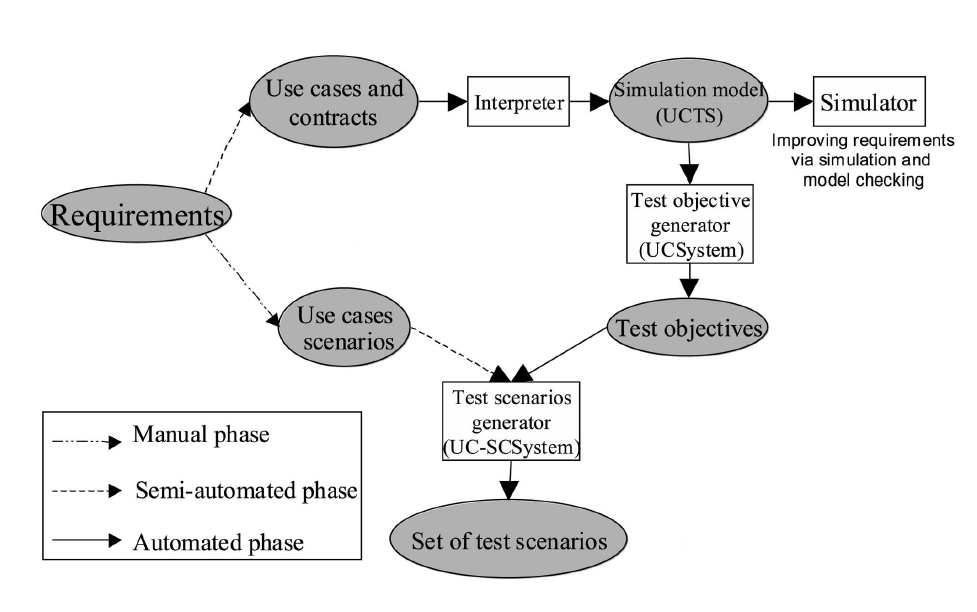
\includegraphics[width=0.75\textwidth]{../images/topic3_transitionsystemflow.png}
	\caption{Flow of generating test scenarios \cite{ClementineNebut2006}}
	\label{tsf}
\end{figure}

The approach consists of two phases (see \autoref{tsf}). In the first phase, UML use cases get enhanced with contracts (pre- and postconditions). Use cases can be seen as the systems' main functions whereas contracts are used to infer the correct partial ordering of functionalities that the system should offer. They express the ordering constraints between the use cases during the simulation process to build the transition system. The contracts are made executable for logical evaluation by writing them in the form of requirement-level first-order logical expressions. They consist of predicates with and are used to describe facts in the system like actor state, main concept state, roles, and more. Each predicate can either evaluate to true or false, but never to undefined. A dedicated editor tool helps to manage the predicates and guides the design of contracts to maintain a nonredundant, minimal set of contracts and predicates. Contracts therefore specify the system properties to make a use case applicable (preconditions) and define the system properties (predicates) acquired after their application (deterministic postconditions). Parameters to use cases can either be system actors or main concepts of the use case, which are represented as normal instantiated objects of classes during the test scenario generation process. 

Through exhaustive simulation by the prototype/interpreter-tool \textit{UC-System} a \textit{use case transition system} (UCTS) is built, which serves as a model for all valid sequences of use cases. Therefore first an initial state and enumerations of different business entities that later serve as parameters to use cases are declared. Then all use cases get instantiated by replacing the set of formal parameters with all the possible combinations of their possible actual values (i.e. actors and main concepts). To apply an instantiated use case the simulation state and the precondition of an instantiated use case must match. The simulation state is then updated according to the postcondition of the contract. The initial state defines which predicates are true from the very beginning, the current simulation state covers all instantiated predicates which are evaluated to true. Now all possible paths are traversed exhaustively until a final UCTS was generated. 

During this step, the requirement engineer has also the chance to check and possibly correct the requirements before the tests are generated. Inconsistencies between predicates and contracts can be identified as well as underspecification or errors in the requirements. Invariants can also be checked. The number of states in the transition system can be calculated with

\begin{equation}
	maxsize_{UCTS} = 2^{n_{ip}}
\end{equation}

where

\begin{equation}
	n_{ip} = p \cdot max_{instances}^{max_{param}}.
\end{equation}

$n_{ip}$ describes the amount of instantiated predicates, $p$ the number of predicates, $max_{instances}$ the maximum amount of instances for a parameter (actors and main concepts of the use case), and $max_{param}$ the maximum amount of parameters per predicate p. In practice, many of the potential states are not reachable and only a small number of instances are necessary for achieving a proper statement coverage. 

Now relevant test objectives get extracted from the UCTS by applying predefined \textit{coverage criteria}. 

The \textit{All Edges} (AE) criterion makes sure that all state transitions are covered, whereas the \textit{All Vertices} (AV) criterion guarantees that all states (predicates) are reached within the set of test objectives.  The \textit{All Instantiated Use Cases} (AIUC) criterion is helpful in case a state transition can be done by multiple use cases or a use case leads to no state change. A combination od AV and AIUC is the \textit{All vertices and All Instantiated Use Cases} (AV-AIUC) criterion. The most strict criterion is probably the \textit{All Precondition Terms} (APT) criterion, which makes sure that all possible ways to apply each use case are exercised. Now, these criteria are mainly introduced to generate functional tests. The \textit{Robustness} criterion on the other hand explicitly exercises a use case in as many different ways as to make its precondition false. Therefore valid test paths are generated, which lead to an invalid application of a use case to generate robustness tests from. All algorithms are based on breadth-first search in the UCTS to obtain small test-objectives that are human-understandable and meaningful. 

\newpage 

Subsequently, in the second phase, test scenarios get generated by replacing each use case in a test objective with the according use case scenario that is compatible in terms of static contract matching. This is done by the prototype-tool \textit{UC-SCSystem}. The use case scenarios were also attached with contracts beforehand. This time the contracts contain more detailed pre- and postconditions. There are contracts that rely on the rest of the model, they are written in \textit{Object Constraint Language} (OCL), and there are contracts that rely on the predicates of the use cases. Now the exchange of messages involved between the environment and the system is also specified. Note that all use case scenarios are system-level scenarios. Eventually, additional parameters and messages need to be passed manually before executable \textit{test cases} can be generated. The process results in executable test scenarios that get evaluated using the statement coverage metric.

One possible challenge of the approach is that the simulation model has to be compact enough to avoid combinatorial explosion of the internal states. Therefore the two-phase approach was chosen and parameters to instantiate use cases during the simulation can often be restricted to only the main system concepts and actors. Furthermore, the above-mentioned test objective generation criteria were identified through experimental comparisons and help to keep the number of test objectives in a reasonable scope. 

The generated test scenarios can either lead to a pass verdict, a fail verdict (in case a postcondition is violated), or an inconclusive verdict. The latter is invoked if a precondition is evaluated to false and the test scenario was not executed entirely. This could be because of underspecification or because of inappropriate test data. To solve this either a new initial state (test data) has to be defined or additional test cases that execute the remaining use case scenarios need to be provided. 

To evaluate the approach the original authors used three software products: An Automated Teller Machine (ATM) with 850 lines of code, an FTP server with 500 lines of code, and a virtual meeting (VM) server with 2.500 lines of code. Statistics on the amount of generated test cases can be found in \autoref{testcases}.

\begin{table}[h] 
	\centering
	\begin{small}
		\caption{Statictics of the generated test cases}
		\label{testcases}
		\setlength{\tabcolsep}{1em}
		\begin{tabular}{l|c|c|c}
			\hline
			& \textbf{ATM} & \textbf{FTP} & \textbf{VM} \\
			\hline
			\# use cases & 5 & 14 & 14 \\
			\hline
			\# nominal UC-scenarios & 5 & 14 & 14 \\
			\hline
			\# exceptional UC-scenarios & 17 & 14 & 14 \\
			\hline
			\# generated functional test cases & 6 & 14 & 15 \\
			\hline
			\# generated robustness test cases & 17 & 33 & 65 \\
			\hline
		\end{tabular}
	\end{small}
\end{table}

Taken the example of the VM server, most coverage criteria reached up to 70\% code coverage, when including robustness test cases even up to 80\%. For more detailed information see \autoref{codecoverage}.

\begin{table}[h]
	\centering
	\begin{small} 
	\caption{Statement coverage reached by the generated test cases}
	\label{codecoverage}
	\setlength{\tabcolsep}{1em}
		\begin{tabular}{l|c|c|c}
			\hline
			& \textbf{ATM} & \textbf{FTP} & \textbf{VM} \\
			\hline	
			\% of functional code covered & 100\% & 90.7\% & 100\% \\
			\hline
			\% of robustness wrt. the spec covered & 42.31\% & 38.6\% & 52\% \\
			\hline
			\% of code covered (total) & 94.76\% & 72.5\% & 80\% \\
			\hline
		\end{tabular}
	\end{small}
\end{table}

All coverage criteria are almost equal in their achieved code coverage, with the exception of the AV criterion. Here the code coverage is low as not all use cases can be covered, especially those use cases that do not change the system state are missing. The ratio between the covered statements and the amount of generated test cases gives information about the efficiency of the generated test scenarios. Here the AIUC and APT criteria scored best. The APT criterion manages to reach 100\% functional code coverage with only 15 test cases. The efficiency of the robustness criterion on the other hand scored quite low, 65 test cases could only cover up to 50\% of the equivalent robustness code. Therefore the approach works well for functional code, but not so well for robustness code. This is because only violations of the use case attached preconditions are taken into account, inappropriate test data, or violating the more detailed preconditions of use case scenarios are not included in the test generation process. 

One possible extension of the approach was also considered. Activity diagrams could be chosen to model the use case dependencies in a more graphical approach, which is then shown in the upcoming approach two. 

\subsection{Application}

In the first step, the test objectives have to be derived. Therefore we define the use cases and their contracts (\autoref{contracts1}) as requirement-level first-order logical expressions. The contracts are used to infer the correct partial ordering of functionalities that the system should offer. Only the use cases that really impact the state of the transition system were specified for this example. The notation used is equal to the one proposed in the paper. \textit{UC} introduces the identifier and parameters of a use case, \textit{pre} marks the beginning of the precondition logical expression and \textit{post} the beginning of the postcondition logical expression. Furthermore, logical operators like \textit{and} and \textit{or}, quantifiers like \textit{forall} and \textit{exists}, and implications by using \textit{implies} can be used. The expression \textit{@pre} ensures that a given logical expression has already been evaluated to true when evaluating the precondition. 

\begin{lstlisting}[caption={Contracts attached to use cases},label={contracts1}]
	
	UC createMovie(m: movie)
	post createdMovie(m)
	
	UC createLinkedPerformer(p: performer, m: movie)
	pre createdMovie(m)
	post createdPerformer(p) and createdLink(p,m)
	
	UC rateMovie(m: movie)
	pre createdMovie(m)
	post calculatedOverallRating(m)
	
	UC ratePerformer(p: performer)
	pre createdPerformer(p)
	post forall(m: movie){ createdLink(p,m)@pre implies calculatedOverallRating(m) }
	
	UC linkExistingMovie(m: movie, p: performer)
	pre createdMovie(m) and createdPerformer(p)
	post not createdLink(p,m)@pre implies (createdLink(p,m) and calculatedOverallRating(m))
	
	UC linkExistingPerformer(m: movie, p: performer)
	pre createdMovie(m) and createdPerformer(p)
	post not createdLink(p,m)@pre implies (createdLink(p,m) and calculatedOverallRating(m))
	
	UC unlinkMovie(m: movie, p: performer)
	pre createdMovie(m) and createdPerformer(p) and createdLink(p,m)
	post calculatedOverallRating(m) and not createdLink(p,m) and not exists(m2: movie){ createdLink(p,m2) }@pre implies not createdPerformer(p)
	
	UC unlinkPerformer(m: movie, p: performer)
	pre createdMovie(m) and createdPerformer(p) and createdLink(p,m)
	post calculatedOverallRating(m) and not createdLink(p,m) and not exists(m2: movie){ createdLink(p,m2) }@pre implies not createdPerformer(p)
	
	UC removeMovie(m: movie)
	pre createdMovie(m)
	post not createdMovie(m) and forall(p: performer){ not createdLink(p,m) } and not exist(m2: movie){ createdLink(p,m2) }@pre implies not createdPerformer(p)
	
	UC removePerformer(p: performer)
	pre createdPerformer(p)
	post not createdPerformer(p) and forall(m: movie){ not createdLink(p,m) and calculatedOverallRating(m) }
\end{lstlisting}

After that, the UC-System prototype/interpreter tool should build the UCTS (\autoref{ucts}) through exhaustive simulation. The pool of parameters was restricted to one movie and performer to avoid a combinatorial explosion for this example. To build instantiated use cases the set of formal parameters are replaced with all the possible combinations of their actual values. In our case, we use the most simple approach by just having one possible combination. Furthermore, the predicate calculatedOverallRating is no longer considered. Note that only predicates that evaluate to true are listed in the states as in the original paper. 

\begin{figure}[h]
	\centering
	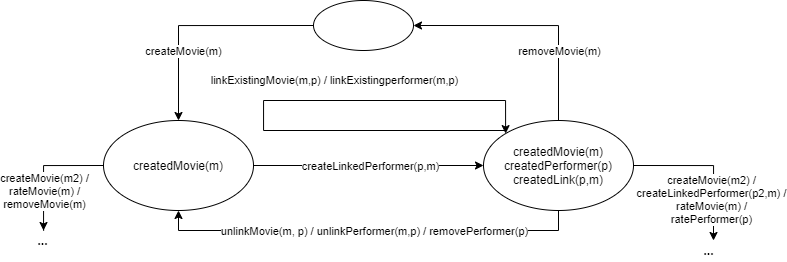
\includegraphics[width=\textwidth]{../images/topic3_ucts.png}
	\caption{The use case transition system}
	\label{ucts}
\end{figure}

\newpage
After applying an instantiated use case in the transition system (in case the precondition of the contract was fulfilled) the simulation state is updated according to the contracts' postcondition. 

Depending on the selected coverage criterion, we receive different test objectives as correct sequences of use cases. The robustness criterion was not considered in this example, but its application is coherent to the functional coverage criteria. How many test objectives are derived depends on the internal implementation of UC-System and cannot be predicted for this example. Let's assume that one test objective is the test path createMovie(m) \mbox{-\textgreater} createLinkedPerformer(p,m) \mbox{-\textgreater} removeMovie(m). Then the use case scenarios from \autoref{ucs} are used to replace the use cases in the test objectives. It helps to specify the exchange of messages involved between the environment and the system.

\begin{figure}[h]
	\centering
	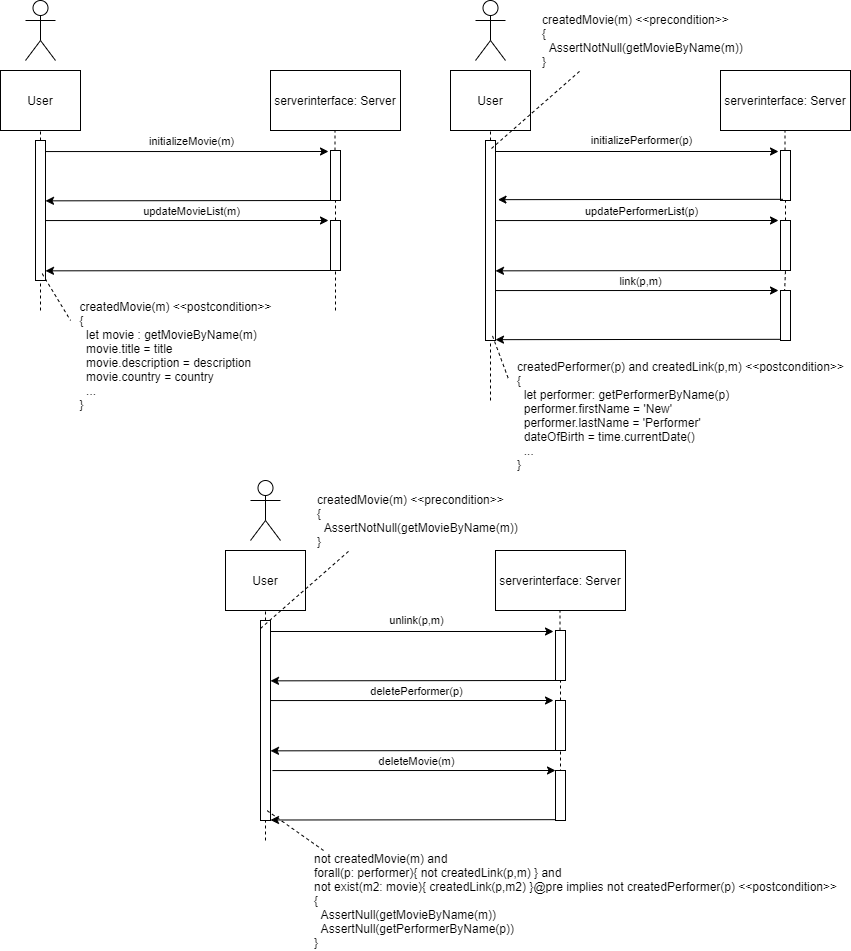
\includegraphics[width=1.0\textwidth]{../images/topic3_ucs.png}
	\caption{The use case scenarios}
	\label{ucs}
\end{figure}

\newpage
Note that the use case scenarios may still be incomplete for the execution. They contain the main messages exchanged between the tester and the SUT and say how the system has to be simulated to perform a use case and how to react to the simulation. To know how the system has to be simulated, the use case scenarios contain more detailed contracts written in OCL besides the contracts written as logical expressions that were provided by the use cases. 

The prototype-tool UC-SCSystem uses the shown implementation in the use case scenarios to derive executable test scenarios as JUnit tests.

\section{Approach 2: An Automated Approach to System Testing based on Scenarios and Operations Contracts} \label{approachtwo}

\subsection{Description}

Based on the suggested improvements in the first paper, the second paper uses a more graphical approach using \textit{interaction overview diagrams} (IOD), a special form of activity diagram used to show control flow, to derive test paths. It helps to start testing in the early stages of development. Each node in the IOD represents either an interaction diagram (sequence diagrams) or interaction occurrences that show an \textit{operation} invocation. Every IOD corresponds to one use case. The IODs get enhanced with contracts written in the \textit{object constraint language} (OCL) and they get transformed into a contracts transition system (CTS) which models all scenarios of the IOD. Here the states are represented by the contracts and the transitions by the operations (interaction diagrams or interaction occurrences) in the IOD. The CTS is built by a tool using the \textit{XML metadata interchange} (XMI) file for the IOD and the operation contracts in OCL as inputs. A state is created against each precondition and each postcondition of the operations. Logical if-then-else conditions are resolved by combining their testing condition with the result, therefore two different sub-states are created. The surrounding postcondition is then a composition of the two sub-states. Additional transitions are added for all conditional flows leading to alternative scenarios and their guard conditions are attached to them. Additional CTS flows help to further refine the requirements by spotting potential unwanted behavior or underspecification. The CTS is often visualized in a matrix. 

Through traversing the CTS test paths get derived. Therefore different coverage criteria are defined. The simplest coverage criterion is the \textit{state coverage} criterion, which generates test paths until all states of the CTS are covered. The criterion is already covered by the wider \textit{transition coverage} criterion, which makes sure that all transitions are traversed before stopping the test path generation. The most expensive criterion is the \textit{transition pair coverage} criterion, each possible transition pair needs to be covered in the test path generation process. It was detected, that the transition coverage criterion delivers a reasonable amount of test paths, but is not suitable for fault detection every time (compared to the transition pair coverage criterion which scores best in this task). 

Besides using a graphical approach with IODs instead of using a formal requirement level language, the key difference to the first paper is that test scenarios do not get generated on system-level but rather on use case level due to the fact that contracts are not attached to use cases (which can be compared to a complete IOD) but rather to all operations within the IODs. It therefore serves as a platform to generate more in-depth test scenarios (as well as for negative test cases). The paper does not provide additional steps on how to generate executable test scenarios from the retrieved test paths. 

\newpage

\subsection{Application}

The second approach differs from the first one as this time a transition system is built on a concrete use case, in our case the use case to unlink a movie from a performer. Input to the approach in this paper is the IOD (\autoref{iod}) with separate contracts defined in an OCL file (\autoref{contracts2}). IODs are a special form of activity diagrams used to show the control flow. The nodes in our case are UML sequence diagrams and define the operations of the CTS. The states are represented by the contracts themselves. 

\begin{figure}[h]
	\centering
	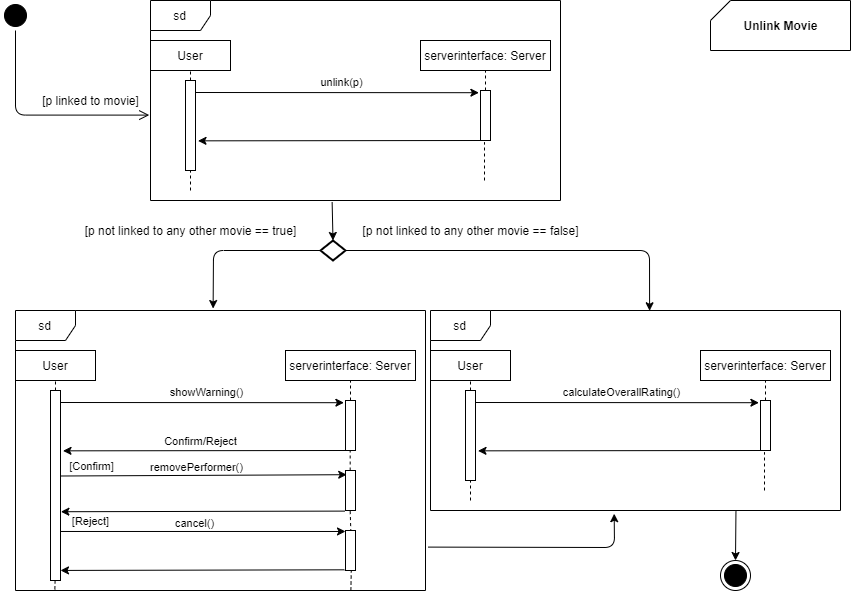
\includegraphics[width=\textwidth]{../images/topic3_iod.png}
	\caption{The interaction overview diagram}
	\label{iod}
\end{figure}

\begin{lstlisting}[caption={Contracts written in OCL},label={contracts2}]
	context Movie::unlink(performer)
	pre  self.performers[performer] -> not isEmpty()
	post self.performers[performer] -> isEmpty()
	
	context MovieManager::removePerformer(performer)
	pre forAll(movie | movie.performers[performer] -> isEmpty())
	post self.performers[performer] -> isEmpty()
	
	context Movie::calculateOverallRating()
	post self.overallRating = 0.5 * (self.mean(self.performers.getRatings()) + self.rating)
\end{lstlisting}

Based on the IOD and the specified contracts the CTS matrix gets defined and leads to the CTS shown in \autoref{cts}.

\begin{longtable}[h]{llll}
	Operations & Pre & Post & Composite States \\
	$O_{1}$ & $S_{0}$ & $S_{1}$ OR $S_{2}$ & A \\
	$O_{2}$ & $S_{1}$ & $S_{3}$ OR $S_{4}$ & B \\
	$O_{3}$ & $S_{3}$ OR $S_{4}$ & $S_{2}$ & \\
	$O_{3}$ & $S_{2}$ & $S_{5}$ & \\
\end{longtable}
The operations (sequence diagrams in the IOD) can be thought of as the transitions in the CTS, whereas the states match the specified postconditions (maybe thought of as starting points of arrows).

\begin{figure}[h]
	\centering
	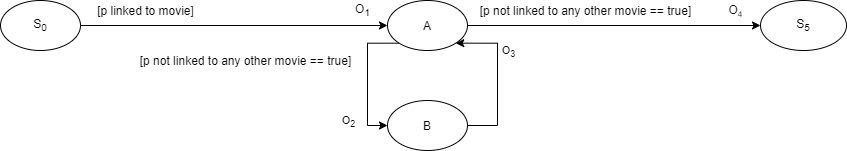
\includegraphics[width=\textwidth]{../images/topic3_cts.png}
	\caption{Contracts Transition System}
	\label{cts}
\end{figure}

For instance, the state $S_{0}$ describes the state when a performer p is linked to the given movie. One can then apply the operation $O_{1}$ to unlink the performer, resulting in the composite state A where either the performer is not linked to any other movie $S_{1}$ or the performer is still linked to another movie $S_{2}$.

Based on a coverage criterion the test paths get derived. Different from the first approach no test scenarios get generated. The paper only shows a new more low-level, graphical approach to generate test paths as this was even a suggested improvement from the authors of the first paper. 

\newpage
\section{Comparison} \label{comparison}
\begin{small}
\begin{longtable}[h]{p{0.45cm}|p{0.425\textwidth}|p{0.425\textwidth}}
	\caption{Synthesis matrix}
	\label{tab3:synthesismatrix}
	\\    %%%%<===
	\hline
	\textbf{No.} & \textbf{Approach 1} & \textbf{Approach 2} \\
	\hline
	1a) & 
	Use cases describing the basic operations in the transition system. Contracts that are attached to the use cases describing the states in the transition system. A contract consists of pre- and postconditions that specify the system properties to make a use case applicable and which properties are acquired by the system after its application. Parameters to contracts are actors and main concepts of the use case. The transition system (UCTS) itself as a simulation model to derive test objectives. The states in the UCTS are given through the predicates defined in the contracts, the transitions are triggered when applying an instantiated use case. Test objectives describing the test paths. Test objectives are derived by traversing the UCTS using a specific coverage criteria. Use case scenarios to build test scenarios from test objectives. Use case scenarios contain the main messages exchanged between the tester and the SUT, they define how the system has to be simulated to perform a use case and how to react to the simulation. & 
	IODs holding all scenarios and operations of a use case. Operations can either be interaction uses or sequence diagrams inside the IOD and define the state transitions. Contracts written in OCL that are attached to the operations describing the states in the transition system. The CTS describing the transition system. Test paths derived from the CTS using coverage criteria.  \\
	\hline
	1b) & 
	Use cases, contracts written as logical expressions, use case scenarios (sequence diagrams), initial system state, selected coverage criterion, and additional use case scenario parameters. & 
	IODs, contracts written in OCL, selected coverage criterion, possibly manual resolving of conflicts in the CTS matrix. \\
	\hline
	1c) &
	To express the ordering constraints between use cases, each use case is attached by a contract. To simulate the use cases, the set of formal parameters of the contracts are replaced with all possible combinations of their actual values. The use cases are then called \textit{instantiated}. To apply an instantiated use case the precondition of its contract must match with the current simulation state. Afterwards the simulation state is updated according to the postcondition of the use case. Exhaustively simulating the system results in the UCTS. To derive test objectives the transition system is traversed according to one of the predefined coverage criteria AE, AV, AIUC, AV-AIUC, or APT. To build test scenarios a use case scenario can replace a use case at a certain stage of execution if the state reached at this stage locally implies the precondition of the use case scenario. Executable test scenarios are generated by the prototype-tool UC-SCSystem. &
	Each operation in the IOD was enriched with its own contract written in OCL. To build the CTS, first all operations have to be identified from the IOD. The operations are taken from the sequence diagrams or from other operations expressed as interaction occurrences in the IOD. Using the contracts of operations, the states for the CTS are identified. Eventually, conflicts in the CTS have to be resolved such as logical if-then-else conditions, equal contract statements, or join nodes. After the CTS was built, test paths are derived from the CTS by applying a coverage criterion, which is either state-, transition- or transition pair coverage. \\
	\hline
	2a) & 
	Automatic test generation from use cases and use case scenarios. Requirement validation by identifying inconsistencies, underspecifications, and invariants. & 
	Deriving test paths from IODs. Further requirement validation on use case level.\\
	\hline
	2b) & 
	Test writers / Developers, Requirement Engineers. &
	Test writers / Developers, Requirement Engineers. \\
	\hline
	2c) &
	Software Requirements (definition of a software requirement, functional requirements, acceptance tests), Software Testing (model-based techniques, objectives of testing, evaluation of the tests performed), Software Engineering Models and Methods (preconditions, postconditions and invariants, behavioral modeling, analysis for consistency, and correctness, traceability). &
	Software Requirements (definition of a software requirement, functional requirements, acceptance tests), Software Testing (model-based techniques), Software Engineering Models and Methods (preconditions, postconditions and invariants, behavioral modeling, analysis for consistency and correctness). \\
	\hline
	3a) & 
	Dedicated editor to design use cases with contracts, UC-System to build the UCTS simulation model, and to derive test objectives from it. UC-SCSystem to exchange the use cases by use case scenarios in order to build the executable test case scenarios. & 
	UML 2.0 as a standard for IODs, OCL as a formal language to write the contracts, prototype tool to derive test paths. \\
	\hline
	3b) & 
	Writing the use cases and contracts is supported by a dedicated editor, but has to be done manually. Deriving test objectives from use cases and contracts through the transition system is done automatically by UC-System. Use case scenarios have to be specified manually, the generation of test scenarios works semi-automatically with UC-SCSystem as it may need additional parameters from the tester. & 
	Only the IOD and contract specification has to be done manually, the complete approach was then automized by a prototype tool. \\
	\hline
	4a) & 
	The approach was evaluated by looking at the statement coverage of three sample programs and the efficiency of test case scenario generation. & 
	The approach was evaluated by looking at the number of test paths generated to cover all success scenarios and fault detections. \\
	\hline
	4b) &
	Code coverage with the most coverage criteria was around 80\%. The coverage criteria differ in efficiency. AE, AV, and AV-AIUC perform with low efficiency, the sets of test cases are larger than in AIUC and APT. APT reaches 100\% functional test coverage with only 15 test case scenarios. Testing robustness leads to a high number of generated test case scenarios that only cover about 50\% of the corresponding code. The approach is good for functional testing, but bad for robustness testing. &
	Using the transition criterion to derive test paths leads to a reasonable amount of test paths and covers all alternative flows in the IOD, but is not suitable for fault detection at any time. The transition pair coverage criterion guarantees the maximum fault detection, but leads to a high amount of test paths. State coverage captures all success scenarios. \\
	\hline
\end{longtable}
\end{small}

Both approaches have a transition system as a core component in common. Both use contracts to define the states in the transition system. A transition can be applied in case the precondition is fulfilled, the state is then updated according to the postcondition. The transition system is used to derive test paths. Furthermore, both approaches define coverage criteria to generate a certain amount of test cases from the transition system. Both have the AE/transition coverage criterion and AV/state coverage criterion in common. Using this core idea it is also easy in both approaches for requirement engineers to validate their specified requirements during the simulation of the transition system. Both papers draw a similar conclusion, that the core approach is helpful to generate functional test case scenarios for the requirements, nevertheless, there is a lack to achieve a comparable coverage for robustness code for fault detection.

Nevertheless, the two approaches differ in their case of application. While \cite{ClementineNebut2006} uses use cases to automatically generate system-level tests, \cite{NajlaRaza2007} restricts to generate test paths for a specific use case. It therefore does not need additional use case scenarios as an input like \cite{ClementineNebut2006} to generate test scenarios as these are already natively given in the IOD. 

Besides the case of application, the input parameters in both approaches are different as well. \cite{ClementineNebut2006} uses requirement-level first-order logical expressions to describe use cases and their contracts. A more graphical approach was chosen in \cite{NajlaRaza2007} by specifying a use case with an IOD instead of using a formal language. 

\cite{ClementineNebut2006} has the special characteristic that it demonstrates an almost fully automized end-to-end test scenario generation process until concrete test execution, which is missing in \cite{NajlaRaza2007}. Nevertheless, this could easily be implemented in \cite{NajlaRaza2007} as well using similar tool support as in \cite{ClementineNebut2006}. 

\section{Conclusion} \label{conclusion}

Testing with a transition system delivers a method on how to bring requirement specification and system test generation closer together, eliminating traceability problems between what was specified and what was implemented. Requirements can easily be validated on their consistency, correctness, and on possible underspecification while at the same time test paths can be derived through traversing the transition system. 

\newpage

In literature search, a second paper besides the given one was found that follows the process of automatically generating test paths through traversing a transition system, but this time uses the in \cite{ClementineNebut2006} proposed extension of IODs as a form of activity diagrams instead of use cases as its input besides contracts. To find this article both snowballing and search-term-based techniques were used, whereas the choice of relevant articles was based on previously specified relevance criteria. Eight resulting papers were found according to these criteria, \cite{NajlaRaza2007} was finally chosen. 

Approach \cite{ClementineNebut2006} almost shows a fully automated way to derive executable test scenarios as JUnit tests. Contract enriched use cases using a formal language based on requirement-level first-order logical expressions are used as an input to the simulation model. Through exhaustive simulation, a transition system is build from which test objectives are derived using coverage criteria. It was empirically proven that the AIUC and APT criterion perform the most efficient and the most extensive measured by statement coverage. Giving contract enriched use case scenarios as a second input helps to generate concrete executable test scenarios. 

\cite{NajlaRaza2007} switches from system level to use case level test generation. It uses contract enriched IODs as graphical input and builds a transition system on it. Test paths are generated using the transition coverage criterion. No further methodology was introduced to generate executable test cases, but as the approach is already specified on use case level, the generation of test code is self-explanatory (a similar tool like UC-SCSystem from \cite{ClementineNebut2006} can be used).

One weakness of both approaches remains the capability to generate a sufficient amount of robustness tests for fault detection. Both approaches only rely on contract violations and do not sufficiently cover data variations as test path generation is only based on one initial state chosen by the test creator. Still, for the automatic generation of functional test scenarios, both approaches show industry-standard and highly applicable solutions.

\chapter{Testing with a timing component}\label{sec:topic_4}

% Tobias_Koch

\section{Introduction}

Requirements are the basis for all testing. In practice, requirements
are often available in a wide variety of formats: As natural language
text, spreadsheets, UML diagrams etc.... In addition to that, requirements
are often not close to testing. In the course of the development phases
of a program, the requirements may expand or change. In industry,
individual software components are often developed by different manufacturers
before they are combined into a system by the client of these productions.
Although components are tested individually and independently, many
errors can only be discovered when the components are integrated.
Therefore Test cases and requirements must be more closely linked.
Flaws and vagueness in requirements are common and hard to discover.
\enquote{On account of this testing time may be wasted with test
cases that result in the detection of flaws in the requirements and
can thus not be used to evaluate the system under test (SUT)}
\cite{Siegl2010}. Therefore requirements must be stricter and more
formal.\\
 Furthermore, there are systems that have to fulfil real-time requirements.
Two approaches ( \hyperref[Chapter]{Chapter~\ref{sec:Approach-1}} and \ref{sec:Approach-2})
will be presented in this chapter. Both approaches test with a time
component as they refer to a real-time system. In these systems, it
is not only important what input the individual system functions receive
(for example, through a boundary value analysis), but also how long
they take. The same input in a real-time system can lead to a different
system reaction if the execution time differs. But not only the execution
duration of a system function, also the time between the execution
of a system function can result in another system reaction. For this
reason, the temporal aspect plays a major role in the approaches.\\
 \\
The first approach with the title \enquote{Model Based Requirements
Analysis and Testing with Timed Usage Models (TUM)} is a graphically
representation of requirements specification. \enquote{During
the creation of the model the requirements are analysed and brought
into an unambiguous and formal representation} \cite{Siegl2010}.
Test cases are automatically generated from the graph using EXAM (Extended
Automation Method). The second approach, \enquote{A Model-Based
Testing Technique for Component-Based Real-Time Embedded Systems}
(in addition to the formal specification of the requirements by models),
deals even more specifically with the dependency between individual
components of SUT, so that they are taken into account in the automatic
test generation from these models.\\
 \\
\hyperref[Chapter]{Chapter~\ref{sec:Literature-Search}} explains the process of the literature
search that was used to find the second approach. \hyperref[Chapter]{Chapter~\ref{sec:Comparison}} 
compares the two approaches and shows the result in a synthesis matrix.
\hyperref[Chapter]{Chapter~\ref{sec:topic_4_Conclusion}} provides an assessment of the approaches
and summarises the most important findings.\\
Please refer to the glossary in order to receive a common understanding of the following terms used in the sections below: CACC, TUM, EXAM, CREMTEG, CIIG, CSIBG, CSIEDBG, AIC, AITC, AIEC.

\section{Literature search\label{sec:Literature-Search}}

The literature search was conducted in too ways: Search term and snowballing.
To find more and possibly different approaches the search question
was chosen to be: \enquote{What models with a timing component
exist that favor the creation of automatically generated tests?}
The ACM \cite*{acm} and IEEE \cite*{ieee} search sources were considered.
Relevance criteria, both substantive and formal, were used to limit
the number of search hits. 
\begin{itemize}
\item Content criteria: \enquote{requirements as a core concept},
\enquote{support for automatically generated tests},
\enquote{model with consideration of timing}. 
\end{itemize}
The content criteria were first searched for throughout the document.
Since the number of hits was too large, the search of the content
criteria was limited to the abstract of the article. 
\begin{itemize}
\item Formal criteria: time criterion, diversity of author and language
of article in English. 
\end{itemize}
The time criterion was initially chosen so that only articles that
were not older than ten years (publication date not less than 2010)
were considered. Since the number of hits was still too large, the
time criterion was finally set to 2015. The difference of the author
from the given article should ensure that a second independent, not
subjectively biased, scientific opinion on the topic \enquote{Testing
with a time component} could be found.\\
Forward Snowballing produced 13 results, two of which were relevant
(according to the criteria). Backward Snowballing also produced 13
results, none of which were relevant. All of the results did not meet
the time criterion, as the given article was from 2010. Table 1.1
shows an overview of the search-term-based literature search.\\
 
\begin{table}[h]
	\centering
	\caption{Overview of the search-term-based literature search}
	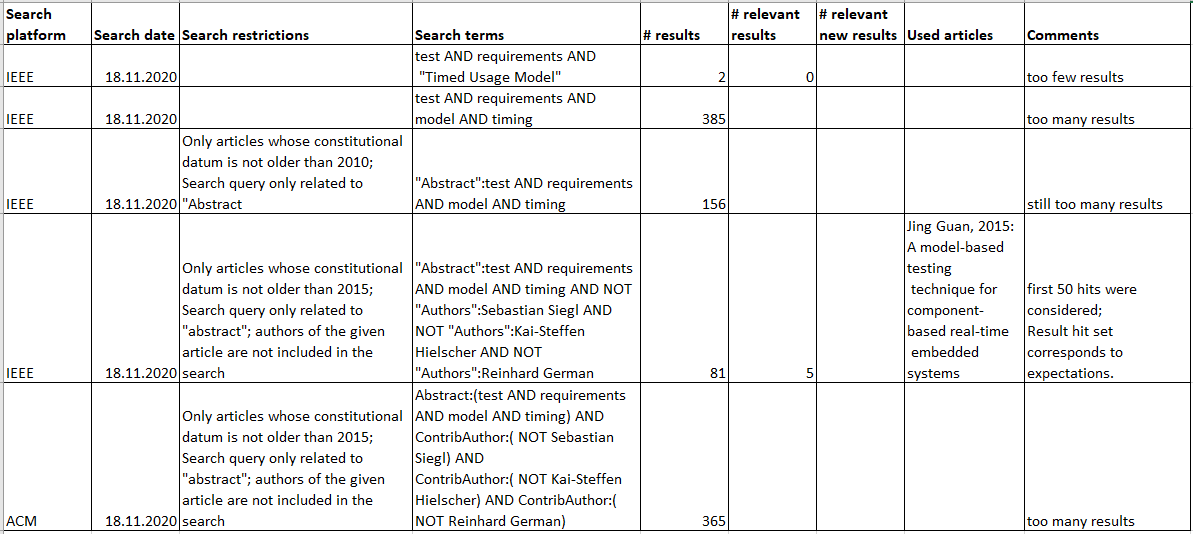
\includegraphics[scale=0.7]{../images/SearchTermTable} 
\end{table}
The search term in the first literature search method used was initially
too specific (test AND requirements AND "Timed Usage
Model"). This was generalised in the next step to increase
the number of hits in the search query: \enquote{test AND requirements
AND model AND timing}. This type of search was able to
optimally fulfill the content criteria and the formal criteria. In
combination with the previously mentioned criteria and the further
restriction of the search that the search term only refers to the
abstract of the article, the literature on which approach 2 is based
was selected.

\section{Approach 1: Model Based Requirements Analysis and Testing with Timed
Usage Models\label{sec:Approach-1}}

\subsection{Description}

In practice, requirements often exist in a wide variety of formats.
A stricter formal notation of the requirements can be achieved through
the so-called TUM (Timed Usage Model). During the creation of the
model, the requirements are analysed and brought into a uniform form.
Each path in the model is ultimately based on a requirement: in this
way, the relationship between the previously created requirements
and the later model-based requirements can be traced at any time.
Each requirement must be simultaneously retrievable in a \enquote{path}
of the TUM. The expected system reaction, after a requirement has
been executed, must be marked in the diagram by means of an (end-)
state. \enquote{Design} errors can be detected early
in the creation of the model. The special feature of the model is
the consideration of the time aspect: The states and state transitions
in the model are each assigned a probability density function (pdf),
which calculates the time how long the system remains in a certain
state or how long the execution of an operation or a response of the
SUT takes. Each state transition is therefore assigned a stimulus,
which represents an operation of the SUT or a system response. 

\autoref{4-1} shows an easy example for a TUM: \enquote{S}
are states, \enquote{a} stands for state transition,
\enquote{t} describes a pdf either with respect
to a state or to a transition, and \enquote{p} describes
the transition probability from one state to the next.

\begin{figure}[H]
	\centering
	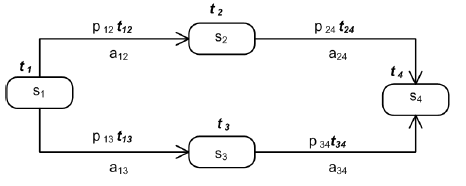
\includegraphics[scale = 1.25]{../images/TUM}
	\caption{TUM \cite{Siegl2010}}
	\label{4-1}
\end{figure}
The model serves as the basis for the entire testing process. It is
used in the testing of real-time systems, e.g. in the automotive industry
or in energy management. The model is created manually using a specially
developed editor. \\
It is done in two steps: First, the system boundary will be defined.
Second, all sequences of stimuli and their responses across the system
boundary will be enumerated \cite{Siegl2010}. All stimuli that go
across this boundary are extracted from the existing requirements
\cite{Siegl2010}. Each possible sequence of stimuli will be mapped
to a response of the system. A response can be composed of one or
more outputs. \enquote{Two sequences u and v are equivalent if
extended by any sequence w the future response is the same to uw and
vw} \cite{Siegl2010}. These equivalent sequences are
reduced to one sequence, since testing the other sequences would be
redundant. In order to maintain an overview of the large number of
all possible sequences, they are listed in order of length: It starts
with an empty sequence \textlambda{}
and all sequences of length one
are created first, then all sequences of length two and so on. By
this procedure a complete and consistent usage model is created. The
finished TUM is passed to EXAM in the next step. \enquote{EXAM
comprises the automated generation of platform dependent code and
the automated execution of the derived test suite without human interactions}
\cite{Siegl2010}. Test cases are automatically generated by running
through the different paths of the TUM. All paths from the start to
the final state are valid test cases.\\
For the test oracle, an appropriate counterpart from the EXAM test
automation library is assigned to each individual stimulus. An importer
allows thereby the import of a requirements library from a document-based
requirements management system. The elements of this system can be
traced back to each individual object in the TUM. The reference values
or the expected result of one \enquote{test path}
for the test oracle can be derived in three different ways: First
automatically generated by computation rules, second by a textual
description (program code or natural language) and third by measurements
and checks on test benches.

\subsection{Application}

The approach \enquote{Model Based Requirements Analysis and Testing
with Timed Usage Models} will now be applied to the Movie Manager,
a collaborative project of students. The program comes with a domain
diagram, an overview of all system functions, and a user task sheet
about movie management in natural language. This data was used in
the creation of the TUM. Data on the transition probability from one
state to the next state is not available. This is therefore considered
to be identical for all state transitions. In order to nevertheless
realise a temporal component in the Movie Manager, the requirements
were extended in the following way: Within the subtasks \enquote{Describe
a movie} and \enquote{Describe a performer},
changes were made to the system functions \enquote{show movie
in IMDB} and \enquote{show performer in IMDB}:
After the error message \enquote{Connection failed}
appears, the system should automatically try to establish a connection
to the IMDB website \cite*{imdb}. If this exceeds a certain time
value (in this case 120 sec.), a final message is issued to the user
stating that the connection could not be re-established automatically.
After this message appears, no further attempts are made to connect
automatically to the IMDB server.

\begin{figure}[H]
	\centering
	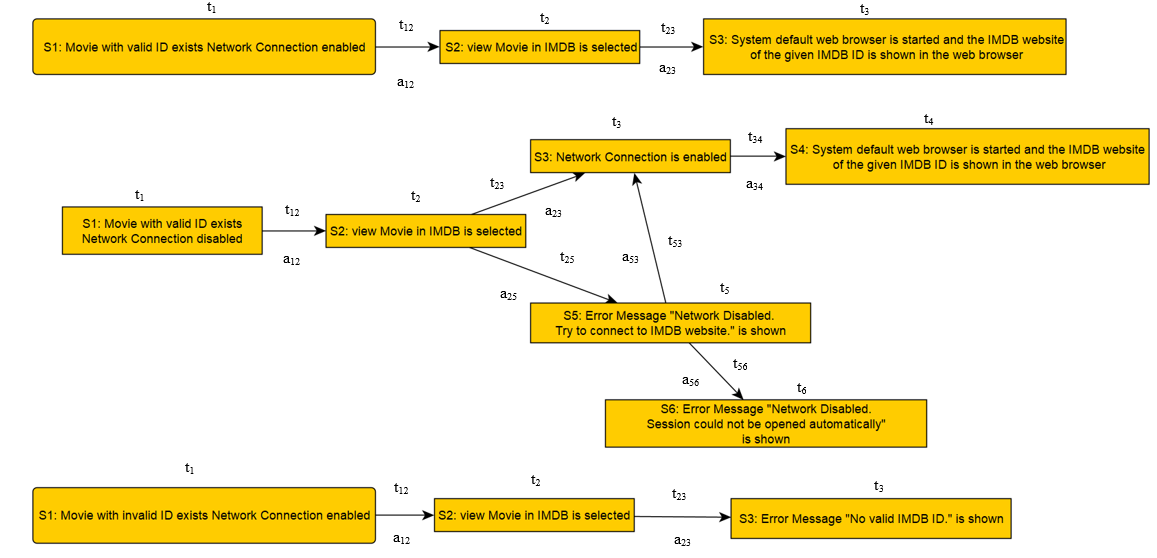
\includegraphics[width=\textwidth]{../images/Application1_MovieManager} 
	\caption{TUM for the systemfunction \enquote{view Movie in IMDB} in Movie Manager}
	\label{4-2}
\end{figure}
\newpage
The middle graph in \autoref{4-2} shows the time dependency: As soon
as t5 \textgreater{} 120 (unit in sec.), the state changes from
S5 to S6. If the network connection has been re-established before
120 sec. have elapsed, the system switches to state S3. The graph
includes all sequences that are conceivable when calling the system
function \enquote{view Movie in IMDB}. In the next
step, a test suite could be automatically created from the graph using
EXAM by traversing all paths in the graph. The exact procedure of
this step is not described in detail in the approach.

\section{Approach 2: A Model-Based Testing Technique for Component-Based Real-Time
Embedded Systems\label{sec:Approach-2}}

\subsection{Description}

Component-based modeling of embedded systems is becoming more and
more important in the field of \enquote{software engineering}
due to the increasing complexity of the systems. The approach now
shows possibilities to improve the quality of tests of component-based
embedded systems by means of several graph-based test models. The
focus is particularly on Non-Functional requirements, more precisely,
real-time requirements. The appropriate testing of these is often
neglected during the integration of the individual components in a
real-time embedded system. The test models presented here (except
for the CIIG (Component Interface Interaction Graph), which only fulfills
the former) take into account not only the functional and temporal
dependencies between individual components, but also the temporal
dependency between state transitions within a component. All the models
presented are created manually using a tool. In the following, it
will be briefly explained how and from which data the models are collected,
which elements they consist of and in which respects they differ.

\begin{figure}[H]
	\centering{}
	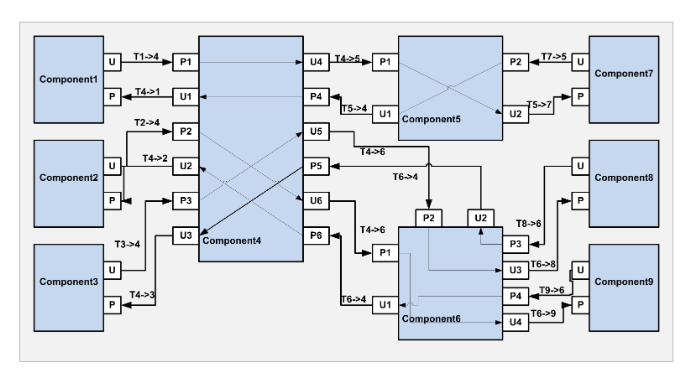
\includegraphics[width=0.9\textwidth]{../images/CIIG}\caption{CIIG \cite{Guan2015}}
	\label{4-3}
\end{figure}
The CIIG, shown in \autoref{4-3}, can be derived from architecture framework
and design specifications, that specify the primary components, interfaces
and dependencies of softwaresystems, for example by context diagrams
or sequence diagrams \cite{Guan2015}. For the CIIG, a component subnet
is created for each component in the sequence diagram. Also, the external
and internal message edges and provider/user interfaces can be derived
from component level sequence diagrams. For each message in the sequence
diagram, a component provider interface, a component user interface
and an external message edge is created. Additionally, one internal
component message edge is created between two external message edges.\\
The CIIG consists of a set of components, which in turn have a certain
number of user (U) and provider interfaces (P). The paths in the model
are defined via so-called message-edges. Internal message edges determine
from which provider interface to which user interface the message
can be sent in a component. External message edges determine from
which user interface to which provider interface the message can be
sent between individual components. Each external message edge is
assigned to a time stamp (for example T1-\textgreater 4), which stores
the transmission time of the message. \\
\enquote{A CIIG represents the time-dependent connectivity relationships
between these components as well as time-dependent relationships inside
a component {[}...{]}. But a CIIG does not reflect the internal behaviour
of a component {[}...{]}} \cite{Guan2015}. This is realized
by a CSIBG (Component State-based Interaction Behavior Graph), shown
in \autoref{4-4}.

\begin{figure}[H]
	\centering
	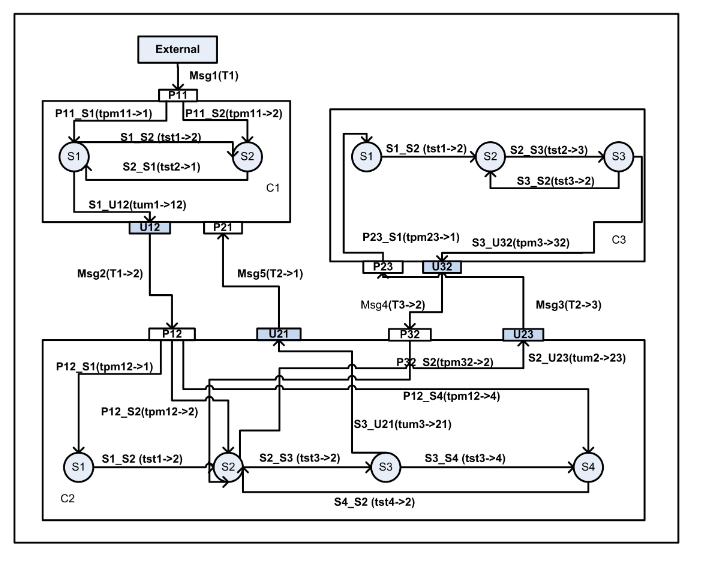
\includegraphics{../images/CSIBG} 
	\caption{CSIBG \cite{Guan2015}}
	\label{4-4}
\end{figure}
\enquote{A CSIBG is created from a CIIG and state transitions
in state diagrams for each corresponding component. Test paths are
generated from the CREMTEG CSIBG diagram {[}...{]}} \cite{Guan2015},
since in this diagram the maximum number of possible paths that can
occur through method calls or state transitions has been created:
The number of test paths is equal to the product of the number of
all possible transition paths in each individual CSIBG component subnet.
In this model, in addition to the CIIG, all internal states (S),
state transitions (for example S1\_S2), transitions between Provider
Interfaces and internal states (for example P12\_S1), transitions
between states and User Interfaces (for example S2\_U23) time
dependencies between individual states (for example tst1-\textgreater
2) and between the states and the provider (for example tpm12-\textgreater
1) or user interfaces (for example tum2-\textgreater 23) of a component
are represented. The most comprehensive model is the CSIEDBG (Component
State-based Event-driven Interaction Behavior Graph).

\begin{figure}[H]
	\centering
	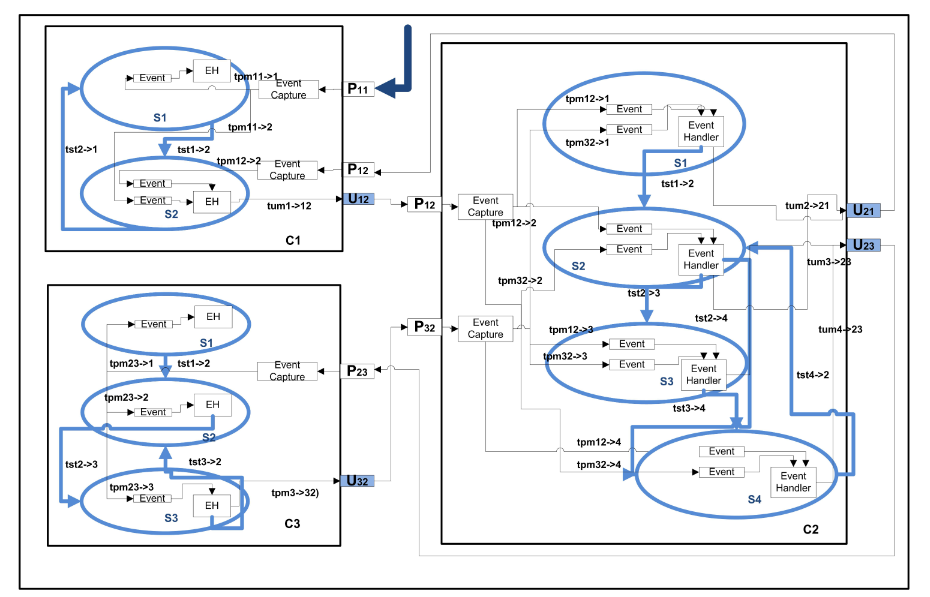
\includegraphics[scale=0.9]{../images/CSIEDBG} 
	\caption{CSIEDBG \cite{Guan2015} }
	\label{4-5}
\end{figure}
\enquote{CIIG and CSIBG clearly described the time sequences
of method calls and paths of state transitions, but they do not deal
with concurrency} \cite{Guan2015}. The CSIEDBG additionally
considers multitasking and non-deterministic behavior, e.g., when
processing simultaneously generated messages. Therefore, the model
in \autoref{4-5} is extended as follows: Each provider service in a component
has one event capture. Each state in a component contains one event
handler (EH) \cite{Guan2015}. \enquote{The provider component
processes the message by event capture to generate events in the current
component state. All generated events are sent to event handler to
decide whether to transition to the next state or send an outgoing
message to the next component {[}...{]}. Decisions in the event handler
are modeled as predicate expressions, where each clause is an event.}
\cite{Guan2015}. New test paths are created according to CACC (Correlated
Active Clause Coverage). CACC is a special form of predicate logic.
For the exact definition of CACC, see the glossary.\\
The models are used to automatically generate test specifications
for component integration testing \cite{Guan2015}. The procedure
is not described in more detail in the approach. The implementation
of the test cases from the test specification is not automated. To
evaluate the suitability of the models, the test suites are run under
a system in which manual errors have been introduced \cite{Guan2015}.
Test Data were hand generated. \enquote{Test data were taken
as inputs to a proprietary test automation tool {[}...{]} . The test
tool reads the input test procedure files, launches the software,
waits for the test to complete, retrieves output log files and analyzes
the results to determine whether test was successful {[}...{]}. A
final test report was generated after all tests were run}
\cite{Guan2015}.\\
The results of the approach have shown that the function and block
coverage and fault detection rate could be significantly improved
by using a CSIEDBG compared to a CIIG or CSIBG. However, in a complex
real-time embedded system, it is often impossible to cover all test
paths. For this reason, it must be decided on a case-by-case basis
which test approach is chosen. Each model fulfills a test criterion
of different quality: A CIIG fulfills the All-Interface Coverage Criterion
(AIC). \enquote{This criterion ensures that each interface is tested once}
\cite{Guan2015}. A CSIBG fulfills the All-Interface-Transition Coverage
Criterion (AITC). \enquote{This criterion ensures that each interface between
components is tested once and each internal state transition path
in a component is toured at least once} \cite{Guan2015}. A CSIEDBG
fulfills the All-Interface-Event Coverage Criterion (AIEC). \enquote{AIEC
combines edge coverage with logical coverage} (see above) \cite{Guan2015}.
Models presented here serve as a basis for the creation of automatically
generated test cases.

\subsection{Application}

The interaction between individual components is now applied to the
Movie Manager Application, shown in \autoref{4-6}. In order to maintain
clarity, the labels above the message edges are omitted as far as
possible. The various widgets within the Movie Manager form the components
in the overall system. Within these components there are states (e.g.
under the component \enquote{Movies Tab} there is
a state \enquote{empty} if no movies are stored
in the movie list and a state \enquote{Movies List}
if at least one movie is stored). The message edges show the information
exchange of the existing system functions. Multi threading does not
play a role in the Movie Manager, so a CSIBG was used for the demonstration.

\begin{figure}[H]
\centering{}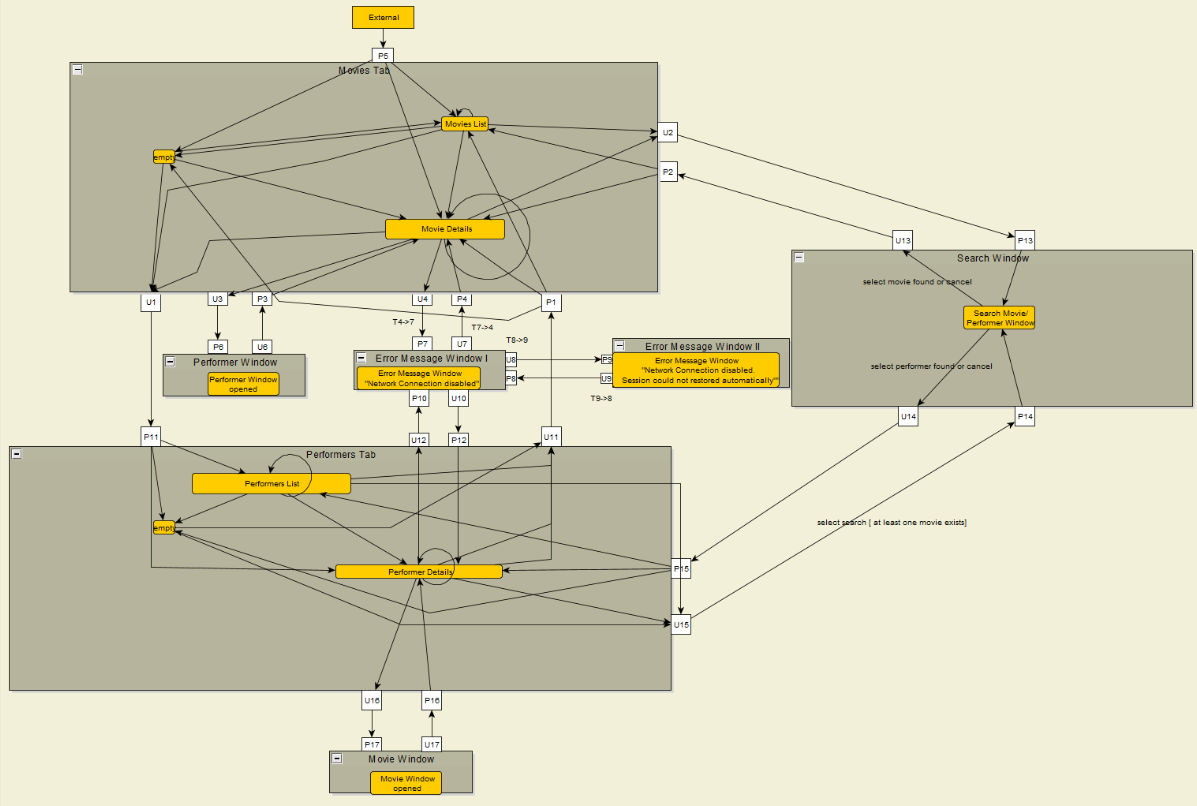
\includegraphics[scale=0.7]{../images/Application2_MovieManager}\caption{CSIBG for the Movie Manager application}
\label{4-6}
\end{figure}

\newpage
Legend for graph shown in \autoref{4-6}: The grey rectangular boxes are
components of the movie manager, the yellow boxes are the states in
a component, the small rectangular boxes on the edge of a component
are User- (U) or Providerinterfaces (P). Arrows symbolize intern (in
a component) and extern (between components) messages. \enquote{T}
are time stamps at external component messages. \\
The system functions \enquote{show Movie in IMDB}
and \enquote{show Performer in IMDB}, which have
already been modified in approach 1, are extended by the following
function: The error message window \enquote{Network Connection
disabled} is to be closed automatically if the network
connection could be restored before 120 seconds have elapsed. For
this example (T7-\textgreater 4) - (T4-\textgreater 7) must be smaller
or equal 120. The Message Edge between U8 and P9 only exists, if (T8-\textgreater
9) - (T4-\textgreater 7) is greater than 120.

\section{Comparison\label{sec:Comparison}}

\begin{small} 		
	\begin{longtable}[h]{p{0.45cm}|p{0.425\textwidth}|p{0.425\textwidth}}
		\caption{Synthesis matrix}
		\\
\hline 
\textbf{No.} & \textbf {Approach 1 (\autoref{sec:Approach-1})}  & \textbf{Approach 2 (\autoref{sec:Approach-2})}\\
\hline 
1a)  & Requirements specification: This could be natural language text, spreadsheets,
drawings or UML charts. TUM: Will be manually derived from the requirements
specification by a special tool. Test Cases: These are automatically
derived from a TUM and executed by EXAM.  & CREMTEGs were manually created with a tool from software architecture
and design specifications (like Graphs, sequence diagrams, state diagrams,
grammars, logical expresses and input domains). The CIIG can be derived
from architecture framework and design specifications, that specify
the primary components, interfaces and dependences of software systems,
for example by context diagrams or sequence diagrams. A CSIBG is created
from a CIIG and state transitions in state diagrams for each corresponding
component. A CSIEDBG is an extended version of the CSIBG. It includes
handling with events for multitasking. Test specifications were automatically
developed from CREMTEGs. An test tool reads the input test procedure
files, launches the software, and waits for the test to complete.\\
\hline 
1b) & Requirements specification in different formats. System boundary is
clearly defined.  & System boundary must (particularly because the approach stays in relation
with an embedded system) clearly be defined. Software architecture
and design specification, from which the data for the models are derived.\\
\hline 
1c)  & The TUM model is created in two steps: First, the system boundary
will be defined. Second, all sequences of stimuli and their responses
across the system boundary will be enumerated. All stimuli that go
across this boundary are extracted from the existing requirements.
Each possible sequence of stimuli will be mapped to a response of
the system. The sequences are created in ascending order of length.
By this procedure a complete and consistent usage model is created.
The finished TUM is passed to EXAM in the next step. After the import,
test cases are automatically generated by running through the different
paths of the TUM. For the test oracle, an appropriate counterpart
from the EXAM test automation library is assigned to each individual
stimulus. An importer allows thereby the import of a requirements
library from a document-based requirements management system. The
elements of this system can be traced back to each individual object
in the TUM.  & First the CREMTEGs will be constructed. For the CIIG, a component
subnet is created for each component in the sequence diagram. A CSIBG
is created from a CIIG and state transitions in state diagrams for
each corresponding component.Test specifications for the test cases
are automatically created from the finished CREMTEGs. The implementation
of the test cases from the test specification is not automated. Finally,
the test cases created from the CREMTEGs are run through in the SUT.
Test Data were hand generated. \enquote{Test data were taken
as inputs to a proprietary test automation tool {[}...{]} . The test
tool reads the input test procedure files, launches the software,
waits for the test to complete, retrieves output log files and analyzes
the results to determine whether test was successful {[}...{]}. A
final test report was generated after all tests were run}\cite{Guan2015}. \\
\hline 
2a) & Automatically generated test cases are created from the requirements;
testing possible at both system and component level. Test time reduced
(through early error detection in requirements and the related incorrect
creation of test cases). Avoidance of ambiguities in the description
of requirements to prevent errors in test creation. Acceptance criteria
such as test coverage can be achieved more easily with the help of
the model. Requirements are less likely to be misunderstood during
software development for the reasons mentioned.  & The basis for the usage scenario is a component-based embedded real-time
system. The test technique is used to put the internal processes (such
as state transitions, event handling) in relation to the required
time and thus create a more transparent test model, which improves
the error detection rate in the system and the general code coverage
of the system.\\
\hline 
2b) & Test designer in the software team, Software developer, Requirements
Engineer  & Test design team (must be familiar with software architecture design
e. g. to analyze UML diagrams, needs advanced domain knowledge)\\
\hline 

2c)  & Software Requirements $\rightarrow$ Requirements Analysis $\rightarrow$
Formal Analysis,

Software Requirements $\rightarrow$ Requirements Validation $\rightarrow$
Model Validation,

Software Testing $\rightarrow$ Test Levels $\rightarrow$ The
Target of Tests,

Software Testing $\rightarrow$ Test Levels $\rightarrow$ Objectives
of Testing,

Software Testing $\rightarrow$ Test Techniques $\rightarrow$
Model-Based Techniques,

Software Engineering $\rightarrow$ Models and Methods $\rightarrow$
Analysis of Models $\rightarrow$ Analyzing for completeness,

Software Engineering $\rightarrow$ Models and Methods $\rightarrow$
Analysis of Models $\rightarrow$ Analyzing for consistency,

Software Engineering $\rightarrow$ Models and Methods $\rightarrow$
Analysis of Models $\rightarrow$ Analyzing for correctness,

Software Engineering $\rightarrow$ Models and Methods $\rightarrow$
Analysis of Models $\rightarrow$ Traceability  & Software Requirements $\rightarrow$ Requirements Analysis $\rightarrow$
Formal Analysis,

Software Requirements $\rightarrow$ Requirements Validation $\rightarrow$
Model Validation,

Software Requirements $\rightarrow$ Requirements Validation $\rightarrow$
Acceptance Tests,

Software Testing $\rightarrow$ Test Levels $\rightarrow$ The
Target of Tests,

Software Testing $\rightarrow$ Test Levels $\rightarrow$ Objectives
of Testing,

Software Testing $\rightarrow$ Test Techniques $\rightarrow$
Model-Based Techniques \\
\hline 
3a)  & An editor for the creation of Timed Usage Models, Requirement Management
System, EXAM, appropriate counterpart from the EXAM test automation
library  & Editor for creating the CREMTEGs, Program for generating automatically
test specifications from CREMTEGs, tool which starts the test and
determines whether test was successful\\
\hline 
3b)  & The creation of the TUMs is achieved using an editor, but must be
generated manually. EXAM includes the automatic generation of platform
dependent code and the automatic execution of the raised test suite
completely without human interaction.  & The CREMTEGs are created manually using an editor. The creation of
the test specification from the CREMTEGs is automated. The implementation
of the test cases from the test specification is not automated. Test
value generation and fault insertion must be done by hand. A tool
starts the test and determines whether test was successful automatically.\\
\hline 
4a) & The approach was evaluated in the testing of a \enquote{start-stop
functionality} (power train functionality) and energy
management in a car. The degree of coverage of the requirements in
manually created test cases was compared with the resulting degree
of coverage in the automatically generated creation of test cases
based on TUM. The advantages of a TUM were already evaluated during
its creation from the requirements.  & The approach was evaluated on an existing component-based embedded
system (satellite communication system written in C and C++, 75000
lines of code). The system was defined using sequence and state diagrams.
The system was then modified by mutation-based fault implementation
to verify the suitability of the design-based test models.\\
\hline 
4b) & The automatic creation of test cases covers a wider range of operation
sequences. The coverage of requirements was systematically increased.
System responses caused by the given functionality were partially
undefined (discovered during the creation of TUM). Requirements were
cleansed of deficits, shortcomings, contradictions and ambiguities.  & The use of extended design-based models in the generation of test
cases achieves a better error detection rate and a higher code coverage
(both function and block coverage) than the manual collection of test
cases. The interaction of internal states of the system (i.e. in the
individual components) could be made more transparent.\\
\hline 
\end{longtable}
\end{small}

Both approaches are presented to automate tests while taking a temporal
component into account. Approach 1 places particular emphasis on analysing
and \enquote{cleaning up} the existing requirements
of ambiguities, deficits and shortcomings. The procedure in this approach
is partly manual, partly automated: TUMs are created from the existing
requirements using an editor. Design errors of the requirements can
be detected during the creation of the model. EXAM allows the automatic
import of the TUM. EXAM generates code for the implementation of the
test cases and executes the test suite automatically. The level of
automation of the approach is therefore very high. In the second approach,
Component-Based Real Time Embedded Model-Based Test Graphs are generated
manually from the existing architecture and design specification.
Similar to the first approach, requirements are unified and thus freed
from ambiguities. Real-time requirements, i.e. requirements that are
linked to a time condition, are the main focus of testing. The level
of detail of a CREMTEG CSIBG or CSIEDBG is significantly higher than
that of a TUM. The special feature of the approach is that for the
first time information from component level sequence diagrams and
statecharts are combined to derive a graph based test model with timing
properties for test generation. From the CREMTEGs, a test specification
for component integration testing can be automatically generated.
The test suite must still be created manually from the test specification.
Test data and seeding of faults in the system are also created manually.
The second approach therefore has a low level of automation. The use
of advanced design-based models (supporting AITC and AIEC) in the
generation of test cases achieves a better fault detection rate and
a higher code coverage (both function and block coverage) than the
method used AIC.

\section{Conclusion\label{sec:topic_4_Conclusion}}

The literature search has shown that the topic of \enquote{testing
with a timing component} is not yet particularly widespread
in the industry. The search query \enquote{test AND requirements
AND Timed Usage Model} yielded only two
search hits, whereby both articles found were by the same author.
The second approach describes that it is very difficult to get access
to running real-time embedded systems, which are necessary to evaluate
the approach. Some intermediate steps have to be done by hand. Therefore,
this approach does not seem to be very mature yet. The test design
team also needs advanced software architecture skills to be able to
analyse UML diagrams. The first approach is a step further in the
automatic creation of executable tests: The TUM is given to EXAM,
which executes all intermediate steps fully automatically until the
test suite is executed. Unfortunately, the text only very sparsely
or not at all discusses EXAM's procedure. However, in both approaches,
the quality of the requirements could be improved considerably through
the use of uniform models.\\
\nocite{*}

\chapter{Testing with a classification tree}\label{sec:topic_5}

\section{Introduction}

If one wants to ensure that all possible cases are covered and checked in a test, the number of test cases can quickly become unmanageably large. If you have a certain number of parameters to consider in your tests, you have to try out and examine every possible combination of these tests to make absolutely sure that no unforeseen problem occurs. If parameters are also continuous, there is also the question of which intervals and values to consider. Depending on the resolution, this can be an unlimited number.

Classification trees (CT) offer an approach to reduce the complexity of such parameter constructions and to keep them clearly arranged. Test cases covering the relevant parameter constructions can then be derived from the CT. This chapter reviews the use of such CTs based on two selected articles describing their uses and suitability.

First, the literature search in the context of classification trees is explained. Subsequently, \autoref{Kap:Approach1} deals with classification trees as a method for creating test cases for model-based systems and discusses them. Using the movie manager as an example, the classification trees are applied to certain requirements. \hyperref[Chapter]{Chapter~\ref{Kap:Approach2}} then introduces Event Sequence Graphs (ESG) as an alternative concept for model-based systems. These are also applied to the movie manager example before a comparison of both approaches takes place in \autoref{Kap:Comparison}. Finally, a conclusion is drawn in \autoref{Kap:Conclusion}. There, we conclude by answering the question of the extent to which CT helped reducing a complex problem to a manageable number of test cases. As with the previous chapters, an attempt is then made to apply the design of this approach to the Movie Manager example.

For a definition of the terms anti-lock braking system (ABS), classification tree (CT), event sequence graph (ESG) and model based black-box testing (MBBBT) please see the glossary. 

\section{Literature search}

The literature search was conducted via snowballing on the given article \enquote{Systematic Model-Based Testing of Embedded Automotive Software} and a keyword search. Two partial approaches were used in snowballing. On the one hand, forward snowballing was used to find articles referencing the first given article. On the other hand, backward snowballing was used to search the articles that are listed by the initial article in the bibliography. Thus, publications directly related to the given article were considered. An overview of the main search results can be found in \autoref{fig:literature_search}. 

\begin{figure}[H]
\centering
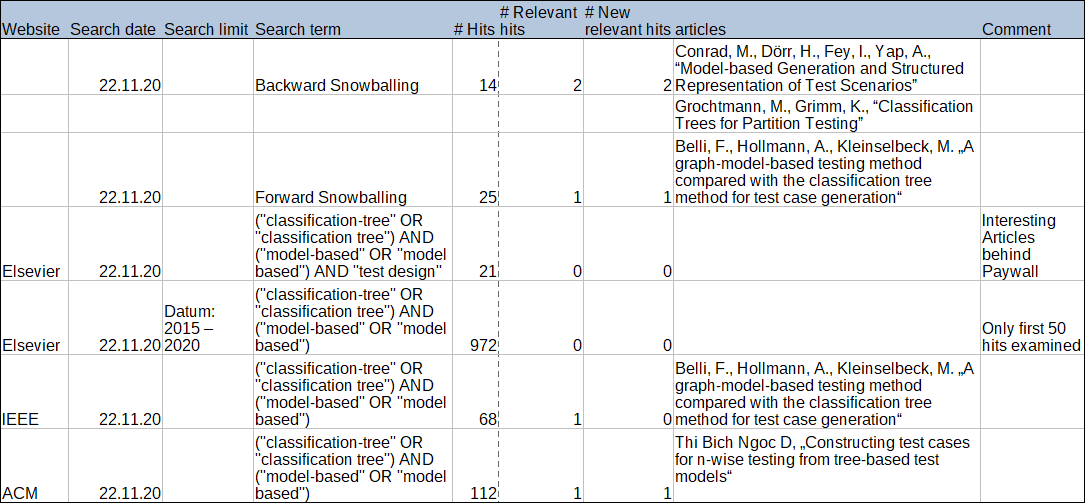
\includegraphics[scale=0.32]{../images/Suchdokumentation_v2.png} 
\caption{The tabular documentation of the search. The relevant results are recorded on the basis of the parameters specified in the columns.}
\label{fig:literature_search}
\end{figure}

A term based search was then performed on Elsevier, IEEE Xplore, and ACM digital library\footnote{The links to the search machines are as followes: Elsevier: https://www.sciencedirect.com/ IEEE: https://ieeexplore.ieee.org/Xplore/home.jsp ACM: https://dl.acm.org/ }. The search query reflects the exact wording that was finally used. During this process, experiments were conducted to estimate which keywords were relevant enough to elicit a suitable number of search hits. In contrary, backward snowballing proceeded without any problems by searching and evaluating the sources listed in the bibliography of the main article in order. Forward snowballing was performed by searching the citations given at Elsevier.

\autoref{fig:literature_search} shows the relevant results of both search methods. The title and abstract of all results have been viewed, aside from the 1000 hits on Elsevier. There, the first fifty results have been considered. The assessment of whether an article is relevant was determined on the basis of three criteria:

\begin{enumerate}
\item CT must be used or described to allow conclusions to be drawn about their suitability
\item The article deals with testing or with the test design
\item The article must be available
\end{enumerate}

The first criterion is intended to filter out articles that do not deal with CT at all and thus do not allow any conclusions to be drawn. The second criterion is to filter out those documents that do not deal thematically with test cases or even software development. Often these articles deal with other types of \enquote{Classification Trees}. An example here are decision trees or graphical visualizations of the classification of objects in artificial intelligence. These trees describe other phenomena or  other problems. However, this chapter is explicitly about the use of such trees for the generation of test cases.

Both approaches to the search yielded multiple hits. One of the articles listed among the relevant search results occurred in the search using both approaches, giving it additional relevance to the topic. Accordingly, the article \enquote{A Graph-Model-Based Testing Method. Compared with the Classification Tree Method for Test Case Generation} by Belli and Hollmann\cite{Belli} has been selected.

\pagebreak

\section{Approach 1: Systematic Model-Based Testing of embedded automotive software}
\label{Kap:Approach1}

\subsection{Description}

The first approach comes from Conrad et al\cite{Conrad}: The article \enquote{Systematic Model-Based Testing of Embedded Automotive Software} deals with the application of CT to problems that have a simulation or model of the application. The application example of the paper is the testing of an Antilock brake system (ABS). Therefore, the introduction starts with a comparison of traditional and model-based software development. \autoref{fig:tradditional_vs_modelbased} from the article shows this difference well. The necessity of model-based test methods is thereby justified. The approach introduced as \enquote{model-based black-box testing} (MBBBT) is presented below. Two perspectives are presented: Requirements-based test design and model-based test design. The basis for this is the creation of a CT.

\begin{figure}[H]
\centering
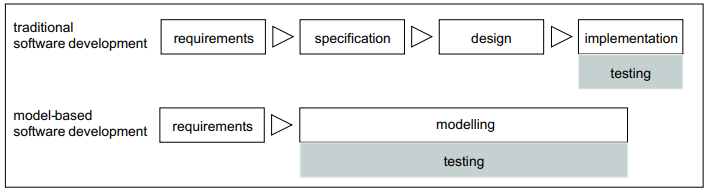
\includegraphics[scale=0.75]{../../individual/groeger/images/TraditionalVSModel.png} 
\caption{This figure from Conrad\cite{Conrad} shows the difference between traditional development and model based developement. They examine CT for projects with a model of the application. \cite{Conrad}}
\label{fig:tradditional_vs_modelbased}
\end{figure}

A graphically represented CT consists of the following components: The root denotes the product or model. The branches derived from it define the classifications. Classifications describe different requirements of the product. This depends on which of the two perspectives mentioned above was chosen as the basis. The leaves of a CT describe the different classes. A class in this context is a qualitative description. Thus, a category is described by the classes here. We can also say the range of values of a category is decomposed into the different classes. \autoref{fig:ABS_CT} shows the requirements-based CT for the ABS model. At the top of the tree are the individual classifications with the different values for the classes. Because this is a requirements-based CT, mostly qualitative descriptions such as \enquote{dry}, \enquote{straight}, or \enquote{strong braking} are found as leaves.  

For the test cases, the combination of these leaves is now to be tested. If you test all combinations of classes of this CT, you cover all test cases defined via the requirements. This assumes that the requirements are complete. In this example, this results in $4*2*3*5 = 120$ combinations.

The next step is the generation of a CT more suitable for the actual model that is used in the developement. Classification now describe different parameters. Classes contain quantitative value or an interval for the input parameters of the model. 

\begin{figure}[H]
\centering
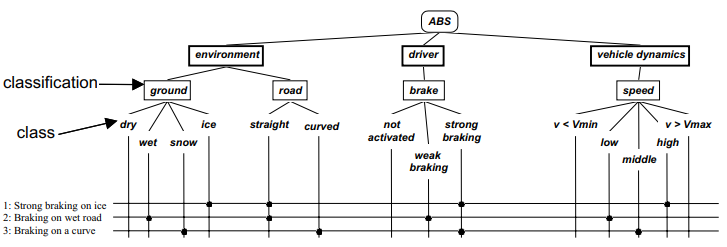
\includegraphics[scale=0.75]{../../individual/groeger/images/ClassificationTreeExample.png} 
\caption{This figure shows the CT made for the use case as presented in \cite{Conrad}. The top part shows the different classifications and classes of the tree while the lower part shows the construction of test cases from the combination of leaf nodes.}
\label{fig:ABS_CT}
\end{figure}

Thus, for both perspectives, a CT is created and compared to analyze whether the requirements are covered by the model-based test scenarios. In this process, the classes of the requirements tree are mapped to the model tree. A model-based tree, on the other hand, describes the input dimensions or model parameters. Qualitative descriptions must therefore be transformed into the input parameters of the model. \cite{Conrad} discusses 1:1 and 1:n relations. 1:1 relations represent unique mappings, while 1:n reflects an occurrence of the corresponding requirement class in multiple parameters of the model. If this mapping is successful, a requirement class can be covered by testing the related classes in the model tree. The relations of the example classes of both the requirement and the model CT are summarized in a table. The summary of \cite{Conrad} explains the advantages of the MBBBT despite higher expenditure by the classification of two different approaches and recommends the application of this approach with the software development with models.

\subsection{Application}

The approach of a CT requires as a basis a model for frequently testing. After the approach of Conrad et al.\cite{Conrad},  requirements, which can be mapped on it, are also needed. Test cases are then determined from this by combining the classes. Tests are conducted with the model. In this example, there is no real, simulatable model to describe it, but there is a description of requirements that could be mapped into a CT. The requirements described are:

\begin{enumerate}
\item Movie	
	\begin{enumerate}
		\item A movie must be able to be added including description.
		\item A movie must be able to be removed
	\end{enumerate}
\item  Performer
	\begin{enumerate}
		\item It must be possible to describe a performer
		\item A performer must be able to be linked to a movie
		\item An actor must be able to be removed
	\end{enumerate}
\item Previous movies
	\begin{enumerate}
		\item Previous movies must be saved
	\end{enumerate}
\item Rating
	\begin{enumerate}
		\item It must be possible to rate a movie
		\item It must be possible to display the rating of a movie
	\end{enumerate}
\end{enumerate}

The CT method appears to be more suitable to single functions. The reason for that is, that the CT makes more sense if all leaf combinations are useful. This is more difficult to achieve if multiple independet functions are achieved. Therefore, the application of the CT approach focuses on the function \enquote{Add and describe performer} as the main functionality of the second requirement. The resulting CT can be found in \autoref{fig:Movie_Maker_CT}. Three questions are important for this functionality: Does the performer already exist? What movies are linked to them? How complete is their description? The function must be able to deal with these different aspects. Therefore, the tree contains these parameters.

\begin{figure}[H]
\centering
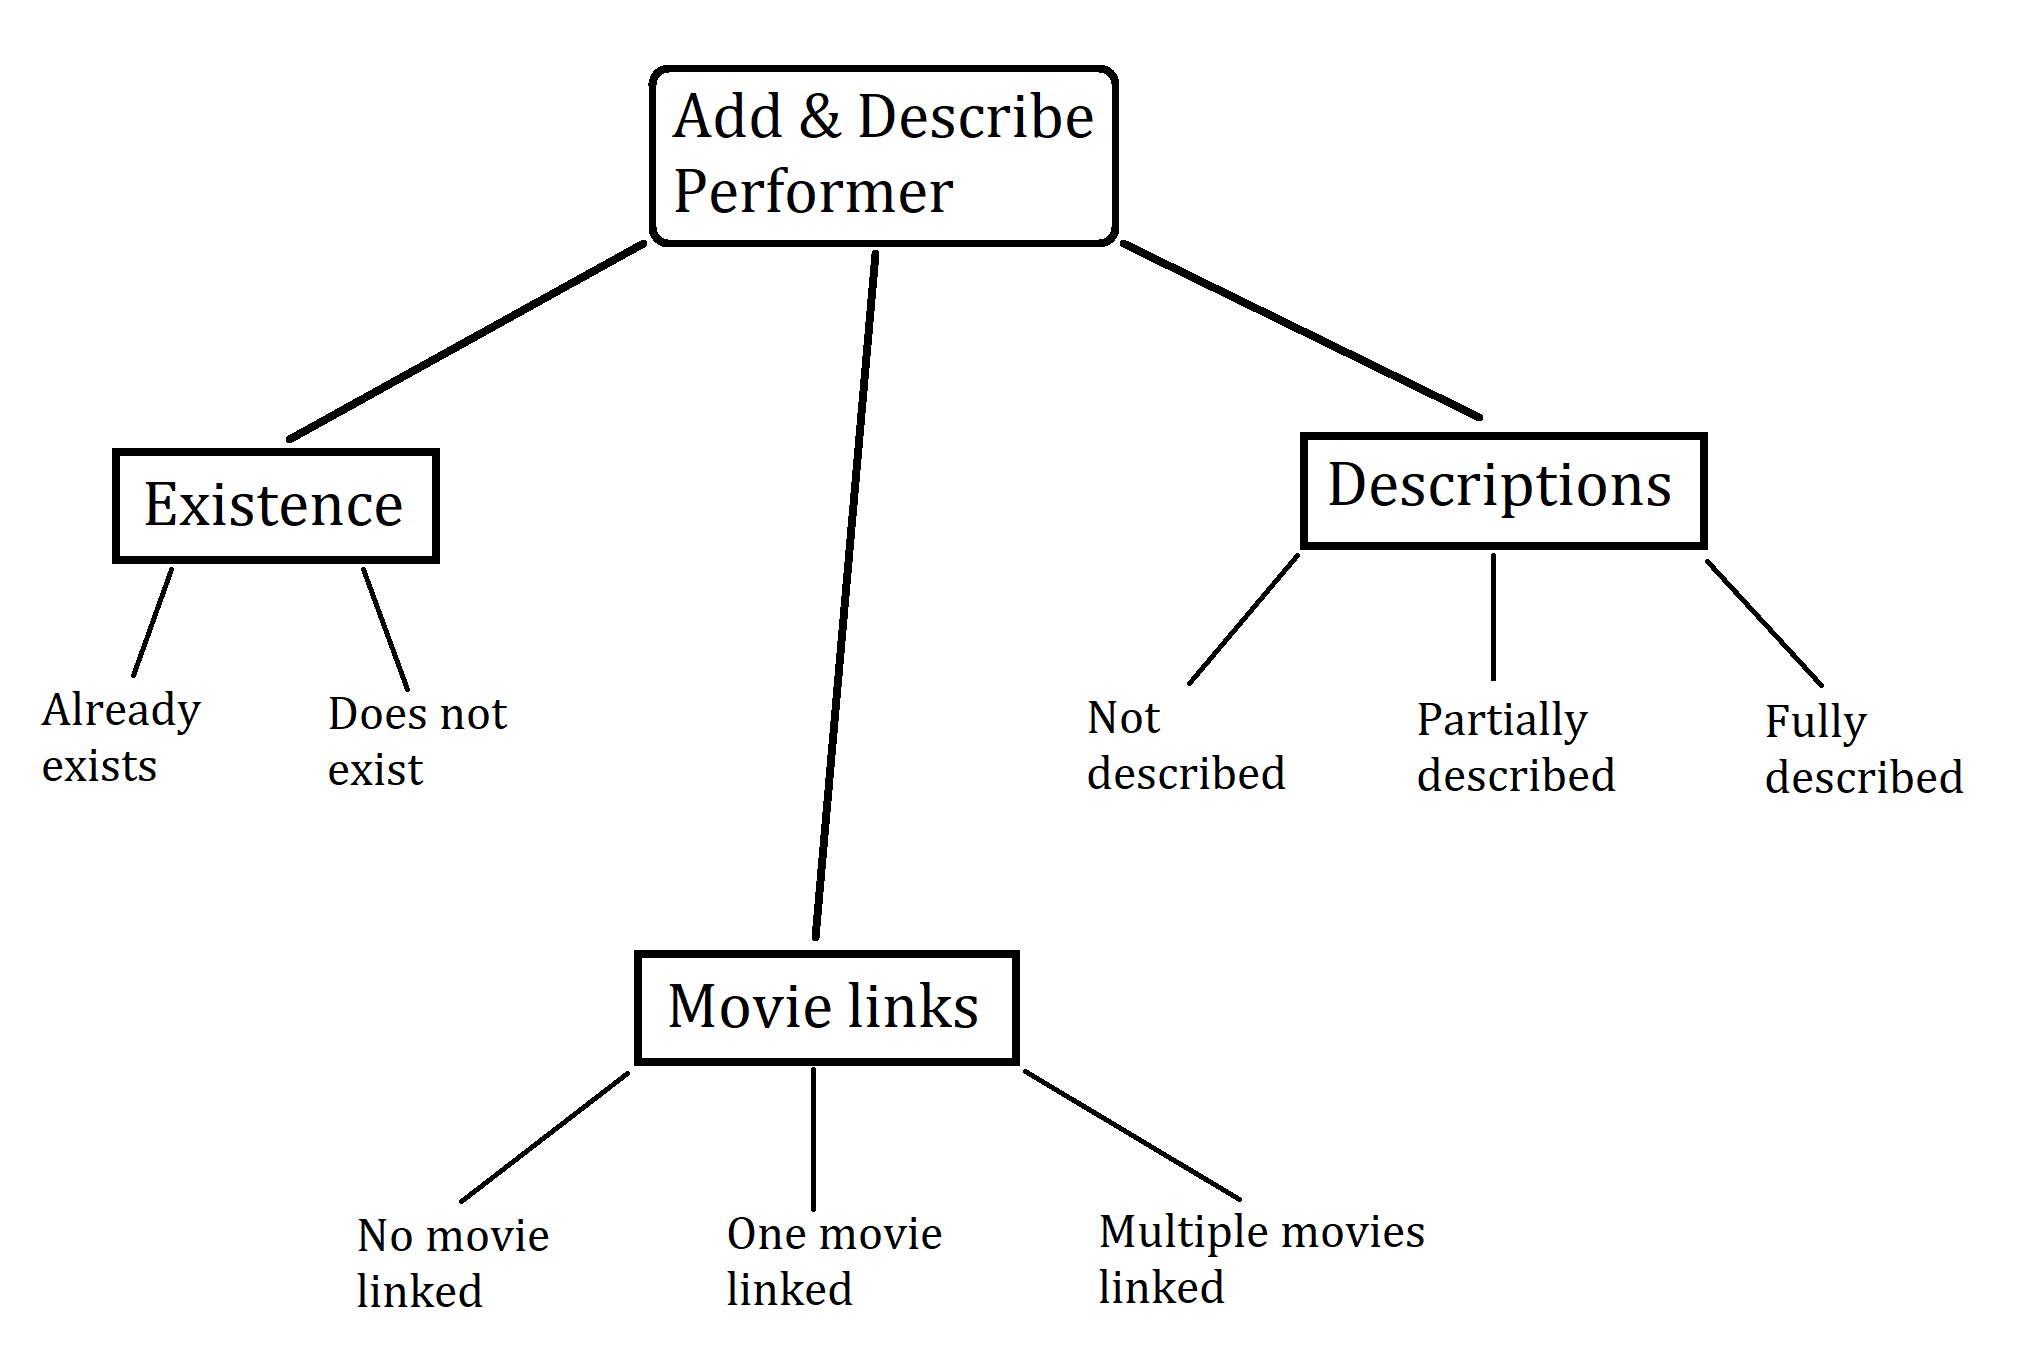
\includegraphics[scale=0.25]{../images/Anforderungsbaum_v2.png} 
\caption{The requirements-based CT for the Movie Manager example defines the various classifications and classes for the test cases. Only a transformation into model parameters has to be done before the test cases can be constructed.}
\label{fig:Movie_Maker_CT}
\end{figure}

In the absence of a proper model against which to make classifications, exactly what counts as input or class depends on the exact implementation. A possible transition to a model based tree according to Conrad et al. \cite{Conrad} can be found in the following table:

\begin{table}[t] 
\centering
%\begin{small}
\caption{A tabular listing of the various requirements with example values. The last column indicates which type of transfer is possible with a suitable implementation.}
\label{tab:ueberfuehrung}

\setlength{\tabcolsep}{1em}
\begin{tabular}{ p{2.4cm}| p{3cm} |p{5cm} |p{1.3cm} }
	\hline
	\textbf{Classification} & \textbf{Class} & \textbf{Model values} & \textbf{Relation} \\
	\hline
	Existence & Already exists & Valid & 1:1 \\
	\hline
	   & Does not exist & NULL & 1:1 \\
	\hline
	Descriptions & Empty & [""] & 1:1 \\
	\hline
	   & Partial & ["Name":"Max M."] & 1:n \\
	\hline
	   & Complete & ["Name" : "Max M.", "release date" : "20XX", ...] & 1:1 \\
	\hline 
	Links & No movie & NULL & 1:1 \\
	\hline 
	   & One movie & ["X: The beginning"] & 1:1 \\
	\hline 
	   & Multiple movies & ["X: The beginning", "X: The continue", ...] & 1:1 \\
	\hline 
\end{tabular}
%\end{small}
\end{table}

The one 1:n relation means, that a partially constructed list can contain different combinations of list entries. These may play a role, so that the model actual needs to test more combinations of partially filled lists. Based on this transition, it is then possible to determine suitable test cases. This results from the combinations of the different classes. Assuming that n is only 1 for the 1:n relation, the classifications for the existence of the performer, the linked movies and the description result in $2*3*3 = 18$ combinations of test cases. Individual test cases can then be, for example, the following:

\begin{itemize}
\item Adding a performer that already exists, without links to movies and a partially filled description, e.g. name and age only.
\item Adding a new performer without details while trying to link him with a movie.
\end{itemize}

These are individual test cases. If you work through all combinations, the tests are considered complete. In some cases, its not necessary to test ALL combinations, since some combinations may not be possible or distinctive. It's heavily depended on the model or the requirements in general.

\section{Approach 2: A Graph-Model-Based Testing Method compared with the Classification Tree Method for Test Case Generation}
\label{Kap:Approach2}

\subsection{Description}

The selected article \enquote{A Graph-Model-Based Testing Method Compared with the Classification Tree Method for Test Case Generation} starts with a description of the difficulties and complexity of testing under time pressure. Quickly, a newer method, \enquote{Event Sequence Graphs} (ESG), is introduced in addition to CT in the context of electronic control unit development. The next chapter explains some basics for this. Besides an explanation of CT, this section also contains a formal description of ESG. Here, a graph with its nodes represents events, including start and end events. Start nodes are the user inputs and end nodes are the final system responses. The graph thus contains valid system flows. Taking any path from start to end event should result in a successful sequence of operations. For each graph a complementary graph can be constructed. The paper also discusses analyzing the complementary graph containing invalid system flows. The article describes valid tests as those that successfully traverse an ESG from start to finish or successfully cause the flows of the complementary graph to fail. \autoref{fig:Approach2_CT} shows a small example of how such a graph may look.

\begin{figure}[H]
\centering
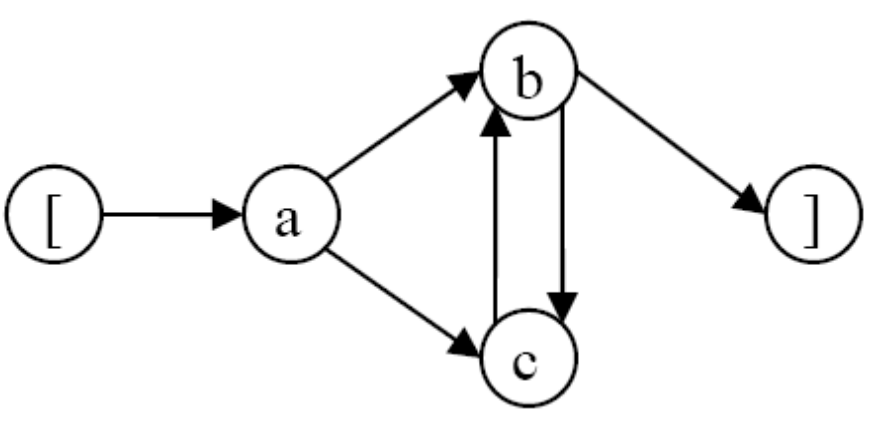
\includegraphics[scale=0.6]{../../individual/groeger/images/ESG_Beispiel.png} 
\caption{A simple ESG as an example from Belli and Hollmann. Nodes with brackets represent start and end events. A successfull test is performed by reaching the end node. \cite{Belli}}
\label{fig:Approach2_CT}
\end{figure}

While CTs look at different combinations of input values, ESGs look at combinations of different sequences of inputs. They then evaluate whether this sequence of \enquote{events} resulted in a success or failure of the action and whether that was part of the expected behavior. Unlike CT, which only looks at what should work, ESGs thus also consider failures.

Then, after the formal description, the test scenario is presented: A control system with ABS, ESP and an adaptive control element. This is followed by a description with specific characteristics of the test environment. The study starts with the application of ESG and CT to the test environment. Difficulties with CT are mentioned, citing dependencies that are difficult to understand. As a result of the study, a lower effort for the creation of CT test, but also a higher number of test cases and thus test steps are mentioned. Both approaches uncovered approximately the same errors. \autoref{fig:Comparison_CG_ESG} shows the main findings of the comparison from Belli and Hollmann's\cite{Belli}'s test study.

\begin{figure}[H]
\centering
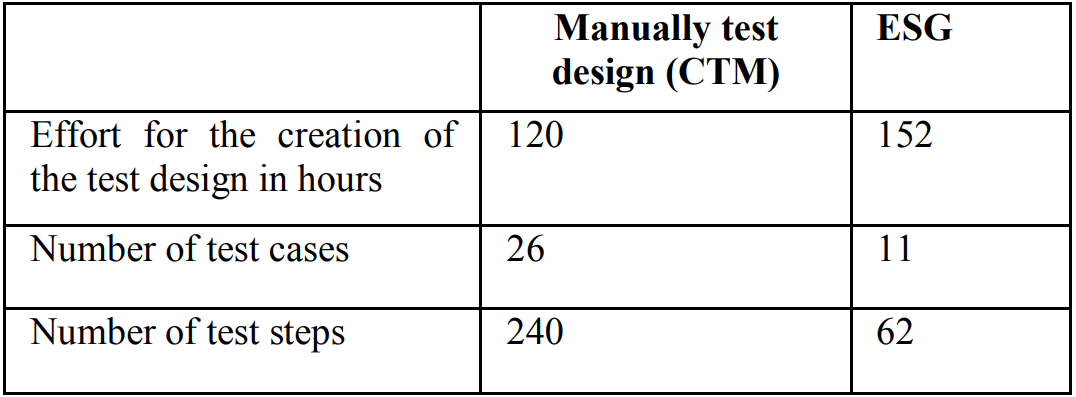
\includegraphics[scale=0.4]{../../individual/groeger/images/Comparison_CG_ESG.png} 
\caption{This table of Belli and Hollmann\cite{Belli} shows the results of the comparison between CT and ESG.}
\label{fig:Comparison_CG_ESG}
\end{figure}

The figure shows the result of the case study performed by Belli and Hollmann\cite{Belli}. According to them, CT and ESG offer their advantages and disadvantages. The effort required for test design is slightly higher for ESGs, while ESGs perform better in terms of the number of test cases and test steps. This shows that CT can at least keep up with ESG in comparison.

\subsection{Application}

The CT, as they are built and used here, are identical in their function. In the article, a model-based CT is built directly without looking at the requirements themselves. This makes it all the more necessary to have a model for simulation or a ready-made application environment. Nevertheless, the same table as in \autoref{fig:Approach1_CT} would arise at this point.

Regarding the ESG, similar difficulties appear when trying to adapt this model based approach to the move manager example. \autoref{fig:ESG_example} shows an example for a partially constructed ESG. Test cases can be constructed by triggering events with Inputs or user actions. Test cases are successful, if they reach the exit event on the right side. Such a test could be: 

\begin{itemize}
	\item 1. Starting with an \enquote{empty data base}
	\item 2. Adding a movie, reaching \enquote{movie exists}
	\item 3. Adding a performer, reaching \enquote{Movie and performer exist}
	\item 4. Linking movie and performer
	\item 5. Closing the application without and error, leading to the exit event.
\end{itemize}

\begin{figure}[H]
\centering
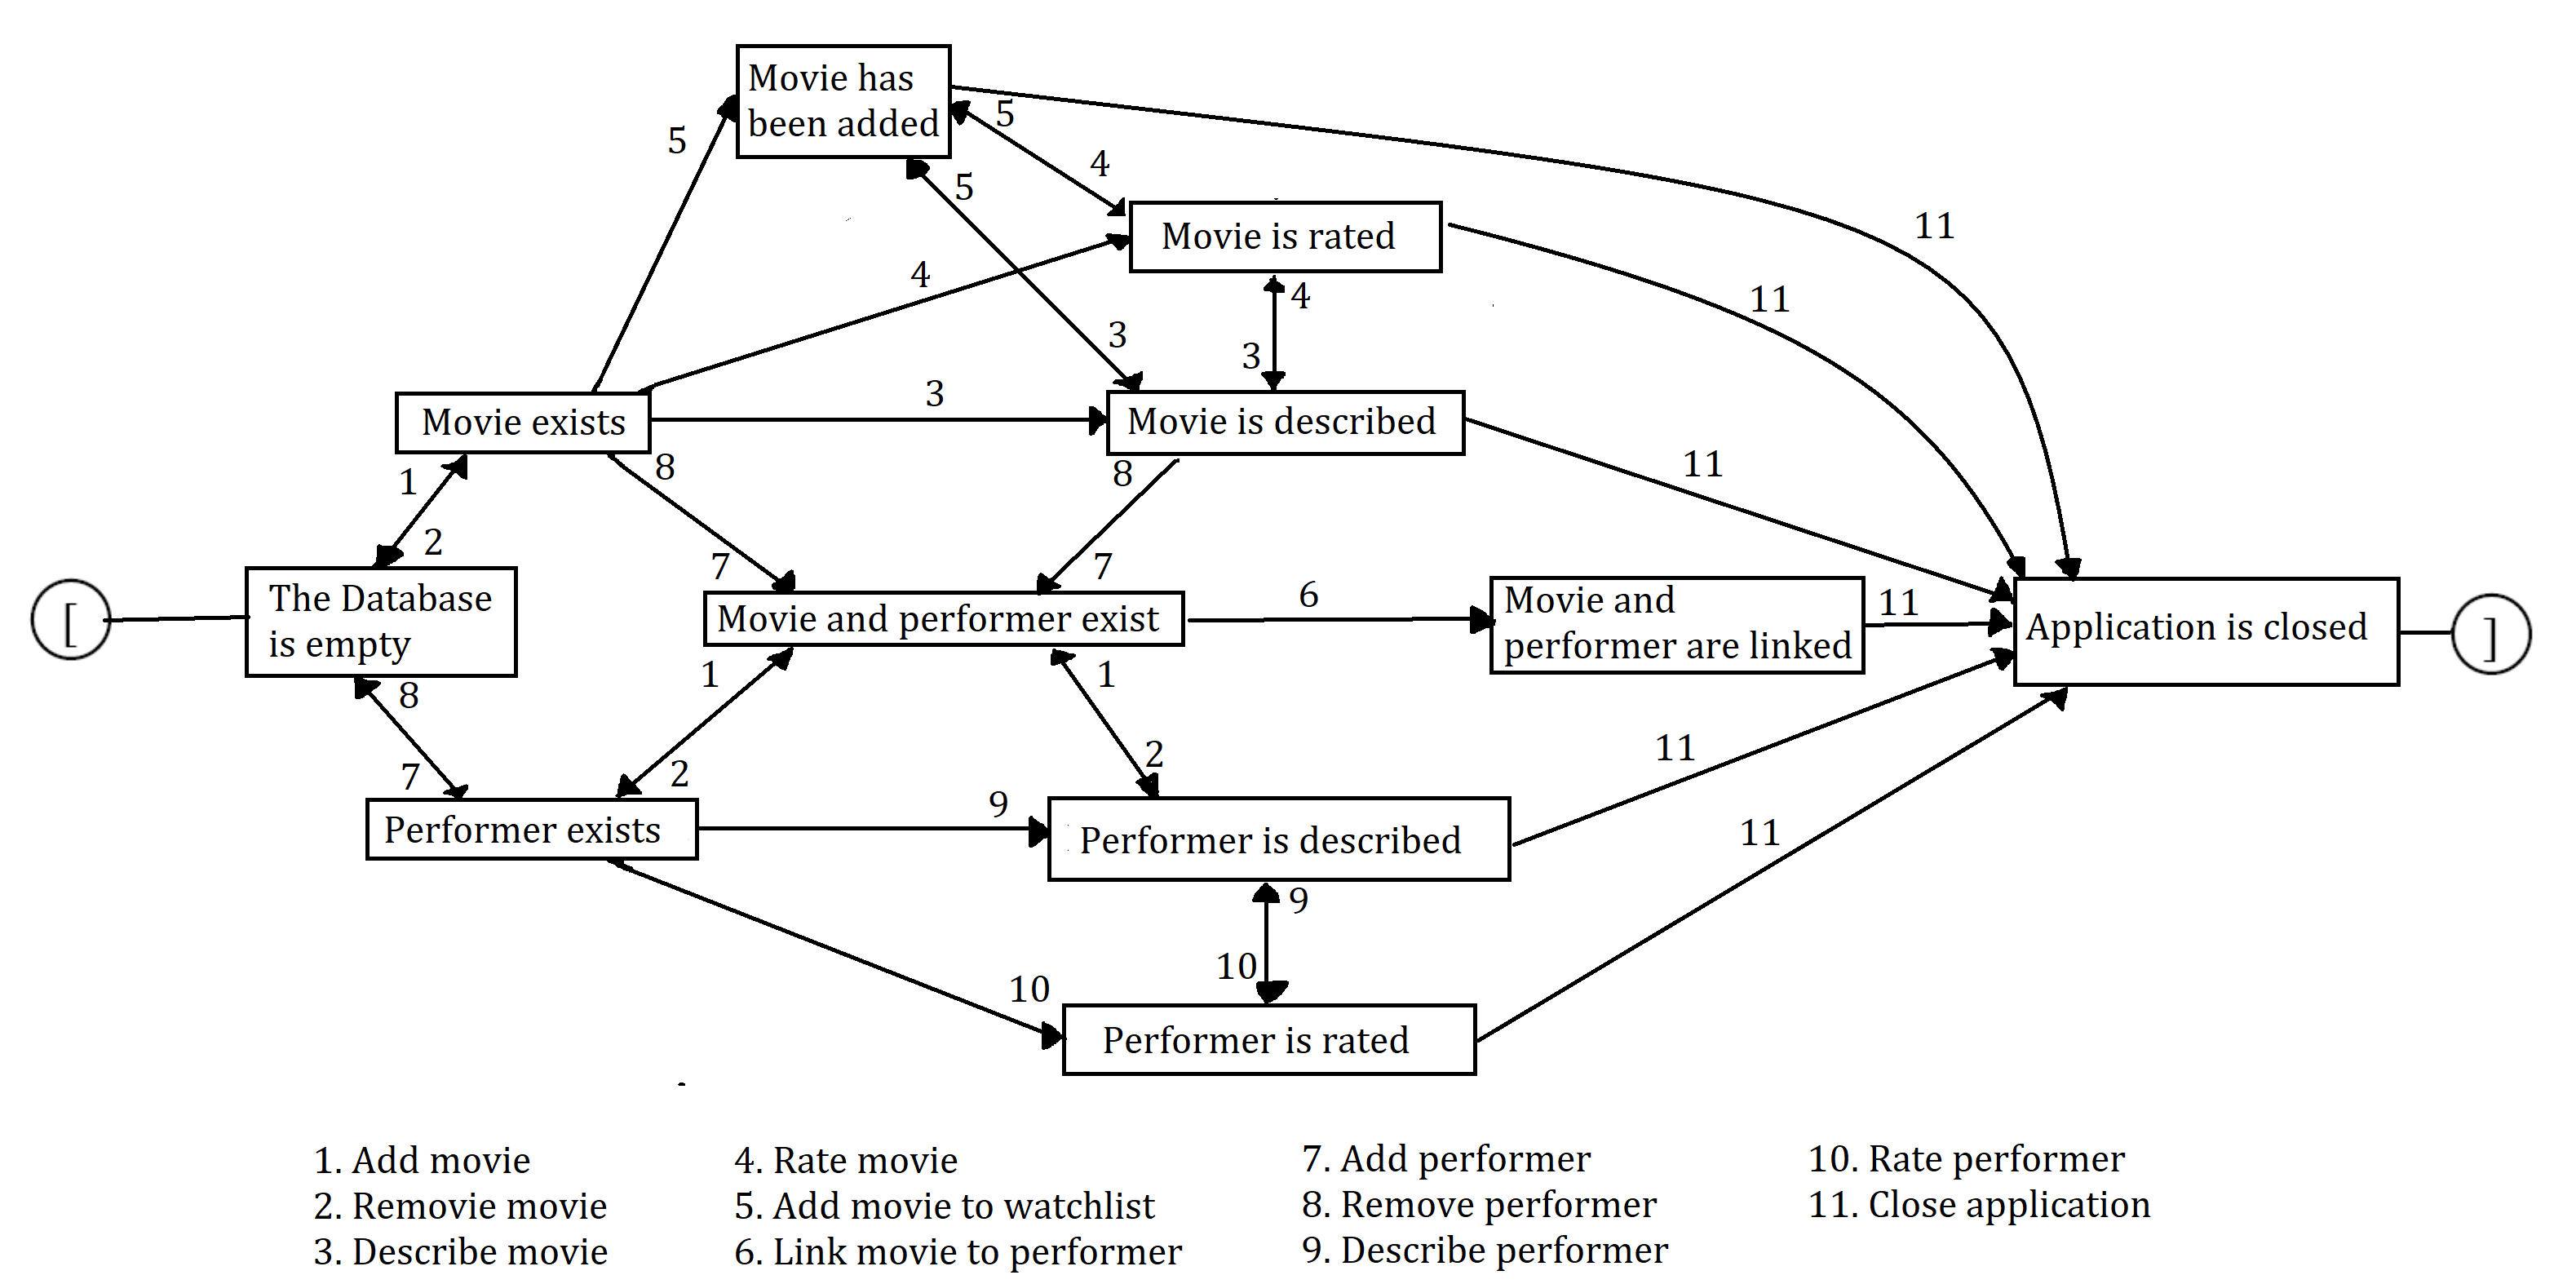
\includegraphics[scale=0.175]{../images/ESGamBeispiel2.png} 
\caption{An example for possible event sequences to construct test cases.}
\label{fig:ESG_example}
\end{figure}

\section{Comparison}
\label{Kap:Comparison}

\begin{small} 		
	\begin{longtable}[h]{p{0.45cm}|p{0.425\textwidth}|p{0.425\textwidth}}
	\caption{The synthesis matrix summarizes the differences, similarities and peculiarities that stood out during the synthesis.}
	\label{tab:synthesematrix_julian}
	\\    %%%%<===
	\hline
	\textbf{No.} & \textbf{Conrad and Fey} & \textbf{Belli et al.} \\
	\hline
	1a) & Anforderungsbasierte CT, Modellbasierte CT,  1:1 und 1:n Relationen & CT, ESG, tabellarischer Vergleich \\
	\hline	
	1b) & Simulierbares Modell liegt vor, Anforderungen können im Modell abgebilded werden & Simulierbares Modell liegt vor \\
	\hline	
	1c) & 1. Entwurf zweier CT für Anforderungen und Modell. 2. Abbildung Anforderungen -> Modell 3. Testentwurf durch Kombination aller Klassen & 1. Entwurf CT und ESG 2. Testentwurf durch Kombination aller Klassen / Zustandsübergänge 3. Vergleich in Tabelle \\
	\hline	
	2a) & Testentwurf mit (black box)-Modellen & Testentwurf mit (black box)-Modellen \\
	\hline	
	2b) & Softwareentwickler, Softwaretester & Softwareentwickler,  Softwaretester  \\
	\hline	
	2c) & Software Testing, Software Maintenance and Software Construction & Software Testing, Software Maintenance \\
	\hline
	3a) & Matlab Simulink & CANoe \\
	\hline
	3b) & 1. Manuell , 2. Manuell , 3. Automatisierbar & 1. Manuell, 2. Vollatomatisierbar, 3. Manuell \\
	\hline	
	4a) & Vergleich der Klassifikationsbäume & 
	Vergleich der Teststatistiken  \\
	\hline	
	4b) & Sehr gut geeignet für black box Modelle auf Basis von Anforderungen & CT sind ein guter Ansatz neben ESG. CT sind schneller zu entwickeln, aber haben größere Tests \\
	\hline	
	\end{longtable}
\end{small}

\newpage
\paragraph{Focus}

In \cite{Conrad}, the special feature is the mapping from requirements-based CT to model-based CT. This is used to ensure that requirements are met by testing a model. From this, a procedure can be derived to formulate a CT from the requirements and apply it to the input parameters of its model or product. In the end, the use of CT for problems with models is recommended. 

In \cite{Belli}, the main focus is the integration of ESG and its comparison with the application of a CT. With this, advantages and disadvantages with related methods can be determined.

\paragraph{Commonalities}

Both approaches deal with the application of CT to model-based test designs. As a result, the prerequisites are similar. The supported usage scenarios and stakeholders are also the same. This is mainly due to the fact that both approaches primarily target an application within the automotive industry. The level of automation is similar in that the test design seems harder to automate due to the level of abstraction.

\paragraph{Differences}

With its focus on the ESG, \cite{Belli} clearly differentiates itself from \cite{Conrad}. As a result, the evaluation also focuses on comparison, while \cite{Conrad} focuses more on usability. Different tools and programs were also used to reach the goal. \cite{Conrad} also goes more intensively into the concept of CT. This is recognizable by the fact that the determination of a CT is dealt with in more detail via a transfer of the requirements.

ESG itself is distinguished from CT, as described in the previous sections, by considering a combination of possible state and input sequences instead of a combination of possible input values, which also makes it possible to ensure that cases that should not work do not work.

\autoref{tab:synthesematrix_julian} shows the synthesis matrix of the two articles on which the comparison of this chapter is based. 

\section{Conclusion}
\label{Kap:Conclusion}

The search on snowballing is promising and also offered relatively many relevant articles. With a term based search, the risk of being flooded with irrelevant hits is greater. This makes sense in that snowballing exploits a direct link via the citations, and free search does not require articles to be related. Thus, articles about decision trees or about testing thematically inappropriate use cases such as medical procedures also appeared among the results. In contrast, one has a wider reach, provided one chooses the search terms appropriately.

Classification Trees offer the possibility to reduce the number of test cases. It turns out that CT are well suited for model-based problems, but it can be difficult to represent arbitrary tasks in this way.  \cite{Conrad} shows for this case how to transform requirements into a CT for the input parameters of a system model. However, the existence of a model-like description remains necessary. According to \cite{Belli}, it is shown that CTs nevertheless remain relevant, even alongside more recent methods. Comparing ESG with CT, Ct appear more suited for a fast classification of input parameters. The approach to derive a CT from given requirements makes it easy to derive test cases. Belli and Hollmans approach with ESG are more complicated to generate. It's harder to make sure to have a complete representation of all states and events as well. The amount of test cases also rises exponentially, since it's a combination of leaf nodes. Therefore, for smaller projects CT seems to be more suitable, while ESG can be helpful for bigger projects.








\chapter{Topic 6}\label{sec:topic_6}

\chapter{Testing with System Models}
\label{sec:topic_7}

In this chapter, we aim to study the topic \textit{testing with  system models}. Section \ref{sec:Intro7} presents the introduction of this topic. Section \ref{sec:LS} describes how the systematic literature research is carried out to identify the existing approaches for testing with system models. In \autoref{sec:AP1}, the first relevant approach for this topic, which is given from the Chair of Software Engineering of University Heidelberg to be studied, is described and implemented on the example application \textit{Movie Manager}. In \autoref{sec:AP2}, the second relevant approach, which is identified through the literature research, is studied likewise. Then, \autoref{sec:Compar} compares the two relevant approaches selected for this topic. In conclusion, \autoref{sec:Conc} presents the insights gained from this study.

In order to get familiar with \textit{system model (SM), test model (TM), model-based testing (MBT), Unified Modeling Language (UML), Systems Modeling Language (SysML)} and \textit{Object Constraint Language (OCL)}, please visit the glossary.


\section{Introduction}
\label{sec:Intro7}

The key to successful product engineering in the software industry today is in many cases a good quality-assurance and deployment of software systems \cite{Paper1}. In order to ensure the quality of a product and verify that the product meets its requirements, we need software testing. 

Model-based testing (MBT) is a software testing technique that has gained much interest in recent years by providing the degree of automation needed for shortening the time required for testing \cite{Paper1}. It provides automatic generation of tests from models representing the behavior of the system under test (SUT) \cite{matera}. From these models, test cases can be derived directly or via some model transformations following different coverage criteria. 

As our topic is testing with system models, it is important to differentiate the two model types \textit{system model} (SM) and \textit{test model} (TM) with respect to the MBT. In our first approach \cite{Paper1}, which is presented in \autoref{sec:AP1}, the authors explicitly stated that they used SMs instead of TMs. And the difference between SM and TM is explained as follows: \enquote{The difference between the two being that the former is both used for development and testing, whereas the latter is only used for testing} \cite{Paper1}. 

In order to discuss the differences between using SM and TM in particularly, the authors of \cite{Paper1} provide with some additional authors the article \textit{Model-Based Testing using System vs. Test Models – What is the Difference?} \cite{SMvsTM}, which is newer than \cite{Paper1} and presents two model-based testing case study examples which use SMs and TMs, respectively. In \cite{SMvsTM}, the SM case study example is our first approach \cite{Paper1} to be studied within this chapter.

The article \cite{SMvsTM} summarizes the differences between the SMs and TMs as shown in \autoref{fig:smtm}.

\begin{figure} [H] 
\centering
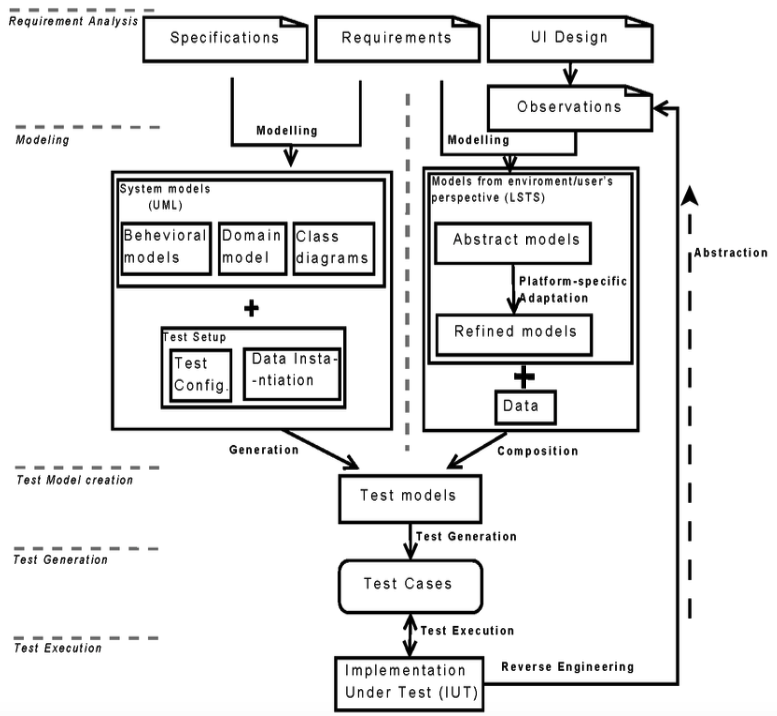
\includegraphics[scale=0.35]{../images/smtm} 
\caption{Sytem models and test models}
\label{fig:smtm}
\end{figure}

From the viewpoint of modeling, one difference between SM and TM is in the way the expected behavior of the SUT is specified with respect to its interfaces; SM provides an internal viewpoint, whereas the TM provides an external viewpoint of the SUT \cite{SMvsTM}. In the terms of reactive systems, TMs provide stimuli and observe the SUT reactions, while the SMs expect the stimuli and provide reactions. Concerning the purpose of modeling, the TMs are developed solely for testing while SMs can be primarily developed for system development (however, SMs are simpler and more abstract than implementation models) and then used for testing as well \cite{SMvsTM}. \\
However, there also some definitions in \cite{SMvsTM}, which conflict with the usage and the way of the models are created in \cite{Paper1}. According to \cite{SMvsTM}, in TM based approaches, implementation is seen as a black-box thus it is hard to give any verdict about how much of the implementation code has been covered by generated test cases unless source code is instrumented for this purpose. Therefore, requirement coverage is mostly used in this case. On the other hand, in SM based approaches, both code and requirement coverage can be observed, again provided that the implementation code is available for such analysis. \\
But as can be seen in \autoref{sec:AP1}, the authors are entirely concerned with the requirement coverage in \cite{Paper1} while using SMs. After stating this, we would like to clarify that for our study we stick to the definition and usage of SM provided in \cite{Paper1}, as it is also suitable with the \autoref{fig:smtm}.

As the SM of the SUT is typically derived from the informal requirements, it is important to trace how different requirements reflect in the models, on different perspectives and on different abstraction levels, and how the generated test cases cover different requirements \cite{Paper1}, \cite{SMvsTM}. For a model-based testing perspective, traceability of requirements means that the generated test cases from the model are linked with the requirements \cite{Paper2}. Thus, traceability of requirements helps to achieve the right level of coverage and shows what requirement has been covered by what test \cite{Paper1}. It also enables us to identify which requirements have been successfully tested and which have resulted in failures \cite{Paper1}. Hereby, traceability of requirements is a pivotal aspect of MBT that allows one to ensure that all requirements have been tested  \cite{matera}.

%\newpage
\section{Literature search}
\label{sec:LS}

This section describes the systematic literature research carried out according to the \textit{Guidelines for Literature Research of the Chair of Software Engineering} \cite{LRGuidelines}. It aims to identify and analyze the scientific articles regarding testing with system models. 

\subsection*{Research question and research strategy}
\label{subsec:RQ}
The main goal of this search is to find relevant approaches for testing with system models, which are similar to the approach provided in the given article \textit{Tracing Requirements in a Model-Based Testing Approach} \cite{Paper1}. 

Based on \cite{Paper1}, which is our start paper for \autoref{sec:topic_7} in this study, we derive the following research question presented in \autoref{tab:RQ}.

\begin{table} [htb] 
\centering
\begin{small}
\caption{Research question and search terms}
\label{tab:RQ}
\setlength{\tabcolsep}{1em}
\begin{tabular}{ l| p{10cm}}
\hline
\textbf{Research Question} & Which approaches exist to generate test cases using system models for the traceability of requirements?\\
\hline
\textbf{Search Terms}  & system model* AND test* AND trac* AND requirement? \\
\hline
\end{tabular}
\end{small}
\end{table}

In order to answer the research question and find relevant articles, we use \enquote{keyword-based search} and \enquote{snowballing} methods. For the keyword-based search method, we determined the search terms as presented in \autoref{tab:RQ}. These search terms were derived from the research question to focus on a certain aspect of the given article \cite{Paper1} and to find a similar approach. 

For the literature research, the digital libraries of the IEEE Xplore (Institute of Electrical and Electronics Engineers) \cite{ieee} and ACM (Association for Computing Machinery) \cite{acm} were used as main sources, since they include the most extensive range of examined scientific publications and are widely recognized. 

In this literature research, keyword-based search method and snowballing search method are conducted to find relevant articles in aforesaid libraries. With keyword-based search method, we search for the search terms presented in \autoref{tab:RQ} with different combinations, since each digital library has a different search method, e.g.  advanced search, or command search.

Snowballing search method is applied to the given article \cite{Paper1} to identify further relevant articles. With backward snowballing method, we go through the reference list of \cite{Paper1} and select the articles as relevant, which fulfill the relevance criteria determined during the literature research. The relevance criteria are presented in \autoref{tab:ArticleCriteria}. With forward snowballing method, we go through the articles, which cite the given article, and again select the articles as relevant, if they fulfill the relevance criteria.

%\subsection{Research Strategy}
%\label{subsec:RS}

\begin{table} [htb] 
\centering
\begin{small}
\caption{Criteria for selecting an article as relevant}
\label{tab:ArticleCriteria}
\setlength{\tabcolsep}{1em}
\begin{tabular}{ l| p{12cm}}
\hline
\textbf{No.} & \textbf{Description} \\
\hline
1 & The article is available in English\\
\hline
2  & The article has a clear focus on software engineering\\
\hline
3  & The article was published in the last fifteen years (2005-2020) \\
\hline
4  &  The article contains an approach for the traceability of requirements using system models to generate test cases, i.e. the article answers the research question\\
\hline
\end{tabular}
\end{small}
\end{table}

In order to ensure that the research methodology and its implementation remain consistent and comprehensible, we formulated four relevance criteria as shown in \autoref{tab:ArticleCriteria}. An article is relevant, if it fulfills all criteria. The first two criteria are formulated to check the availability and the subject area of the articles. Since this work is to be written in English, the article to be used should be available in English. To reduce the comprehensive subject area to the relevant area for our topic, the article should have a clear focus on the area of software engineering as described in the second criterion. The third criterion aims to focus on recent work and to limit the search results. The last criterion is formulated to answer the research question and to find relevant articles, which particularly provide similar approaches to the approach presented in \cite{Paper1}.

\subsection*{Research execution and literature results}
\label{subsec:RE}

First, the search was carried out using the keyword-based search method with aforesaid search terms. In \autoref{tab:ResultKeyword}, the results of this search are documented.\\
First column shows the search location, second column shows the date on which the search was carried out, and third column shows the applied restriction of search. Fourth column presents the exact search query of the search terms and thus shows how they were searched in the specified parts of articles. Fifth column shows the number of overall results, and sixth column shows the number of relevant articles. Finally, last column presents the number of articles chosen to be used in this study.

\begin{table} [H] 
\begin{small}
  \begin{center}
  \begin{scriptsize}
\caption{Results of the keyword-based search method}
\label{tab:ResultKeyword}
\begin{tabular}{   m{1cm} | m{1cm} | m{1.6cm} | m{4.8cm} | m{1cm} | m{1.2cm} | m{0.7cm}  }
\hline
\textbf{Search Location} & \textbf{Search Date} & \textbf{Restriction}  & \textbf{Search Terms}  &  \textbf{\# Results}  & \textbf{\# Relevant Articles}  &  \textbf{Used Results} \\
\hline
IEEE & 20.11.20 & 2005-2020, Advanced Search & ((((\enquote{Full Text Only}:\enquote{system model*}) AND \enquote{Document Title}:test*) AND \enquote{Abstract}:trac*) AND \enquote{Full Text Only}:requirement?) & 64 & 2 & 0\\
\hline
ACM & 20.11.20 & 2005-2020, Advanced Search & $[$Full Text: \enquote{system model*}$]$ AND $[$Publication Title: test* $]$ AND $[$Abstract: trac*$]$ AND $[$Full Text: requirement?$]$ AND $[$Publication Date: (01/01/2005 TO 12/31/2020)$]$ & 9 & 0 & 0\\
\hline
ACM & 21.11.20 & 2005-2020, Advanced Search & $[$Abstract: system model*$]$ AND $[$Publication Title: test*$]$ AND  $[$Abstract: trac*$]$ AND $[$Abstract: requirement?$]$ AND $[$Publication Date: (01/01/2005 TO 12/31/2020)$]$ & 46 & 2 & 0 \\
\hline
IEEE & 21.11.20 & 2005-2020, Advanced Search & ((((\enquote{Abstract}:system model*) AND \enquote{Abstract}:requirement?) AND \enquote{Abstract}:trac*) AND \enquote{Document Title}:test*) & 59 & 0 & 0\\
\hline
\end{tabular}
\end{scriptsize}
 \end{center}
\end{small}
\end{table}
\newpage
As shown in \autoref{tab:ResultKeyword}, in all of our searches we searched the search term \enquote{test*}  in the \textit{documentation title} part, and the search term \enquote{trac*} in the \textit{abstract} part of the digital libraries, in order to find the closest approaches as possible to the presented approach in \cite{Paper1}. Although the \enquote{system model} is the most important search term for this topic, it was not written even in the abstract of the given article \cite{Paper1}. Therefore, with considering that, we decided to search this term also in the \textit{full text} part, instead of only in the \textit{abstract} part of the digital libraries. Consequently, the search terms \enquote{system model} and \enquote{requirement} were searched in the first searches only in \textit{full text} part, then in the second searches in \textit{abstract} part of the digital libraries. 

After identifying relevant articles by using keyword-based search method, snowballing method was conducted to the \cite{Paper1}, which is our start paper for this study, in order to find further relevant articles. The results of the search using snowballing method are detailed documented in \autoref{tab:ResultSnowballing}.

\begin{table} [H] 
\begin{small}
\begin{center}
\begin{scriptsize}
\caption{Results of the snowballing search method}
\label{tab:ResultSnowballing}
\begin{tabular}{  m{1.2cm} | m{4.7cm} | m{1.3cm} | m{1.6cm} | m{1.7cm} | m{1.2cm} }
\hline
\textbf{Search Date} & \textbf{Reference} & \textbf{Direction}  & \textbf{Number of Citations}  &  \textbf{\# Relevant Articles}  &  \textbf{Used Results} \\
\hline
\multirow{2}{1.2cm}{19.11.20} &  \multirow{2}{4.7cm}{\cite{Paper1} Tracing Requirements in a Model-Based Testing Approach} & Backward & 15 &  1 &1  \\ \cline{3-6} & & Forward &11 &1 & 0\\ 
\hline
\end{tabular}
\end{scriptsize}
 \end{center}
	\end{small}
\end{table}

Thus, after conducting the keyword-based and snowballing search methods, we could identify six relevant articles presented in \autoref{tab:RelevantArticles}.

\begin{table} [H] 
	\begin{small}
  \begin{center}
  \begin{scriptsize}
\caption{Results of the literature search}
\label{tab:RelevantArticles}
\begin{tabular}{  m{0.5cm} | m{4.7cm} | m{4.6cm} | m{1.2cm} | m{1.2cm}  }
\hline
\textbf{ID} & \textbf{Title} & \textbf{Authors} & \textbf{Year}  & \textbf{Source}  \\
\hline
\cite{Paper1}&Tracing Requirements in a Model-Based Testing Approach & F. Abbors, D. Truscan and J. Lilius, & 2009 & IEEE \\
\hline
\cite{matera}& MATERA - An Integrated Framework for Model-Based Testing& F. Abbors, D. Truscan and A. Baecklund & 2010 & IEEE\\
\hline
\cite{Relevant3} & A Subset of Precise UML for Model-Based Testing &F. Bouquet, C. Grandpierre, B. Legeard, F. Peureux, N. Vacelet, and M. Utting&2007&ACM \\
\hline
\cite{Relevant4}& Requirements Traceability in Automated Test Generation - Application to Smart Card Software Validation & F. Bouquet, E. Jaffuel, B. Legeard, F. Peureux, and M. Utting&2005&ACM \\
\hline
\cite{SMvsTM} & Model-Based Testing using System vs. Test Models – What is the Difference? &  F. Abbors, D. Truscan, J. Lilius, M. Katara, H. Virtanen, A. Jaeaeskelaeinen, and Q. A. Malik& 2010&IEEE\\
\hline
\cite{Paper2} & Requirements Traceability in the Model-Based Testing Process &Eddy Bernard and Bruno Legeard & 2007&DBLP\tablefootnote{dblp computer science bibliography \url{https://dblp.uni-trier.de/}} \\
\hline
\end{tabular}
\end{scriptsize}
 \end{center}
\end{small}
\end{table}
The articles \cite{Paper1}, \cite{matera}, \cite{Relevant3}  and \cite{Relevant4} were identified through the keyword-based search method, and \cite{SMvsTM} and \cite{Paper2} were identified through the snowballing search method. The first identified article \cite{Paper1} through the keyword-based search method was already given us for this study as start paper. Since \cite{matera} and \cite{SMvsTM} are from the same author group of \cite{Paper1}, we didn't choose them for our study as a second approach to examine. 
\newpage
The articles \cite{Relevant3} and \cite{Relevant4} have also common authors, and one of them is the same author of the article \cite{Paper2}. Therefore, we excluded the \cite{Relevant3} and \cite{Relevant4}, and chose only \cite{Paper2}, \textit{Requirements Traceability in the Model-Based Testing Process}, which is closest to the provided approach in the given article \cite{Paper1}, and very suitable for our topic \textit{testing with system models}.

Consequently, \textbf{\textit{Tracing Requirements in a Model-Based Testing Approach}} \cite{Paper1} and \textbf{\textit{Requirements Traceability in the Model-Based Testing Process}}  \cite{Paper2} are the chosen articles to be studied in this \autoref{sec:topic_7}.


\section{Approach 1: Tracing Requirements in a Model-Based Testing Approach}
\label{sec:AP1}

This section describes the approach presented in \textit{Tracing Requirements in a Model-Based Testing Approach} \cite{Paper1}, and its application on the \textit{Movie Manager}, which is an application used by private individuals at home to manage their own film collection \cite{MovieManager}. What this management includes is described as sub-tasks in the user task sheet of Movie Manager in \cite{MovieManager}. 

\subsection{Description}
\label{subsec:DE1}
This approach was presented in 2009 by Fredrik Abbors, Dragos Truscan, and Johan Lilius in \cite{Paper1} for tracing product requirements across a model-based testing process. With this approach, the authors show how the informal requirements of the SUT evolve and are traced to system specifications and from system specification to tests during the test generation process. They also show how the test results are analyzed and traced back the specification of the system. 
%The approach is only described using small examples from a telecommunications case study. In that case, the SUT is a mobile switching server (MSS), which is a network element located in a mobile telecommunication system. The MSS is responsible for keeping track of the location of mobile subscribes (MS) in the network and for connecting calls between MS’s over 2G and 3G networks. The MSS is also responsible for tracking the movement of MS’s during an ongoing call\\
%Figure~\ref{fig:Ap1-1} presents the model-based testing process of this approach.\\

\begin{figure} [h] 
\centering
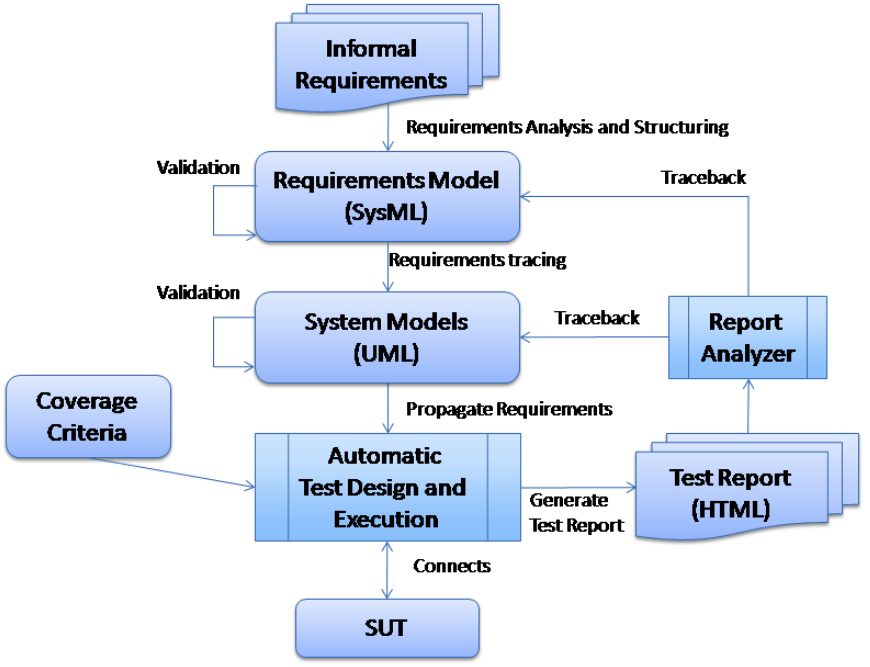
\includegraphics[scale=0.3]{../images/Ap1-1.png} 
\caption{Overview of the model-based testing process \cite{Paper1} }
\label{fig:Ap1-1}
\end{figure}

As shown in \autoref{fig:Ap1-1}, the model-based testing process starts with the analysis and structuring of the informal requirements (including protocol specifications, standards, user scenarios, etc.) into a \textit{requirements model} via Systems Modeling Language (SysML). Because compared to the pure textual description of requirements, a requirement diagram offers several advantages due to its visual overview, e.g. missing aspects can be easily identified to help identify additional requirements, and the different types of relationships facilitate traceability and promote understanding \cite{netreqdia}. Requirements traceability is built on top of this testing process, since authors want to be able to trace how different parts of the system models relate to the requirements and then to see how different requirements are covered by the generated test cases. Another reason for tracing requirements is that if a requirement changes, it is essential to know how this change is reflected in the models. Therefore, after requirements are structured hierarchically using SysML requirements diagrams, they are traced to different models or parts of the models implementing them. 
 
%Secondly, once the test report becomes available, we would like to be able to identify which requirements have been successfully tested and which have resulted in failures. In addition, for the failed test cases we should be able to trace back from test cases those parts of the SUT specification that generated the failure.
For the modeling, the Unified Modeling Language (UML) is used to specify the SUT. For a successful test derivation, several perspectives of the SUT are modeled; a class diagram is used to specify a \textit{domain model}, a \textit{behavioral model} is used to describe the behavior of the SUT, \textit{data models} are used to describe the message types exchanged between different domain entities, and \textit{domain configuration models} are used to represent specific test configurations using object diagrams. In order to increase the quality of the resulting models, a set of modeling guidelines and validation rules are defined. These rules ensure that the models are consistent with each other and moreover, that they contain the information needed in the later phases of the testing process. For editing the SysML and UML models and for running these validation rules, the NoMagic’s \textit{MagicDraw}\footnote{NoMagic MagicDraw \url{https://www.nomagic.com/products/magicdraw}} tool has been used. 

When all requirements have been linked to model elements and the models have been validated, the models used to specify the SUT are subsequently transformed into input for an automated test derivation tool for model driven testing, \textit{Conformiq Qtronic}\footnote{Conformiq Qtronic \url{https://www.conformiq.com/}}, via an automated transformation. Qtronic accepts as input a SM of the SUT from which it automatically designs test cases according to the selected coverage criteria. The input model can be expressed as a combination of UML state machines \cite{SMvsTM} and the transformation basically translates these UML models to the Qtronic Modeling Language (QML), a textual specification language with a Java-like syntax used by Qtronic for specifying the SUT. There are two main purposes for modeling behavior using state machines. First, by using UML state machines the behavioral properties of SUT specification are formally verified. Second, Qtronic tool expects the behavior of SUT in the form of state machines \cite{traqml}. During the transformation from UML to QML, links between requirements and model elements are preserved. 

In this approach, only the online testing mode of this Qtronic is used, in which tests are generated and applied on-the-fly against the SUT. For test generation, different coverage criteria types can be manually selected from the graphical user interface (GUI) of Qtronic like requirements, state, transitions, paths, conditional, or statement coverage. The generated test cases are sequences of input/output messages and their data values derived from the SMs to be sent/received by the SUT \cite{SMvsTM}. As the designed test cases are at the same abstraction level as the SM, an adapter is used to concretize the tests \cite{SMvsTM}. One-by-one Qtronic generates an input message, sends it via the adapter to the SUT, and generates a new input message based on the responses from the SUT. A logging back-end can be used during test execution. The logging back-end provides connectivity to the Qtronic reporting infrastructure and it is used by Qtronic to generate a test report. Three logging back-ends are provided by default. With these logging back-ends, Qtronic can generate test reports in HTML, SQLite, and XML format. When all tests have been applied against the SUT, Qtronic generates a test report in the chosen format, which summarizes the results of the testing process in terms of generated test cases, verdicts, coverage levels, requirements traceability matrix, etc. Unfortunately, the rest of the automatic test generation and execution process of this approach was not provided by the authors. 

With this approach, it is also possible to trace-back requirements from test cases to models. For this purpose, the rest report is analyzed and the information of the failed test cases is collected. Then, the requirements attached to those test cases are traced back to system models. This enables to identify which requirements were not validated during testing and to what parts of the specification they are linked. A Python script was developed by the authors that automatically analyzes the Qtronic test report. 

According to the authors, the provided approach proved beneficial through the fact that many errors have been detected in the early stages of the process, when the system models have been created. For instance \cite{SMvsTM}, some errors originated from inconsistencies discovered in the SM, which were due to misunderstanding of requirements or to incomplete validation of models before testing. Other errors have been found in the adapter, as well as in the SUT.

Furthermore, it should be noted that although Conformiq is still active and offering different kind of products for an end-to-end test automation, its Qtronic product mentioned in this approach is not existing in Conformiq's current product list. Unfortunately, after our research, we could not find any information about what happened to Qtronic. Therefore, we assume that it was not developed further.





\subsection{Application}

%As presented in Figure~\ref{fig:Ap1-s1}, 
First, functional requirements of the SUT should be analyzed and structured into requirements models using the requirements diagrams of SysML. Each requirement element contains a \textit{name} field which specifies the name of the requirement, an \textit{id} field that simply specifies the id of the requirement, a \textit{text} field which describes the requirement, and a \textit{source} field which specifies the origins of the requirement. The source can be a link to or a name of a textual document from where the requirement has been extracted. 

In our implementation, we converted the user sub-tasks of Movie Manager into system functions in order to build a requirements diagram from system functional requirements. \autoref{fig:Ap1-req} presents the example of a SysML requirements diagram for our application. 


\begin{figure} [h] 
\centering
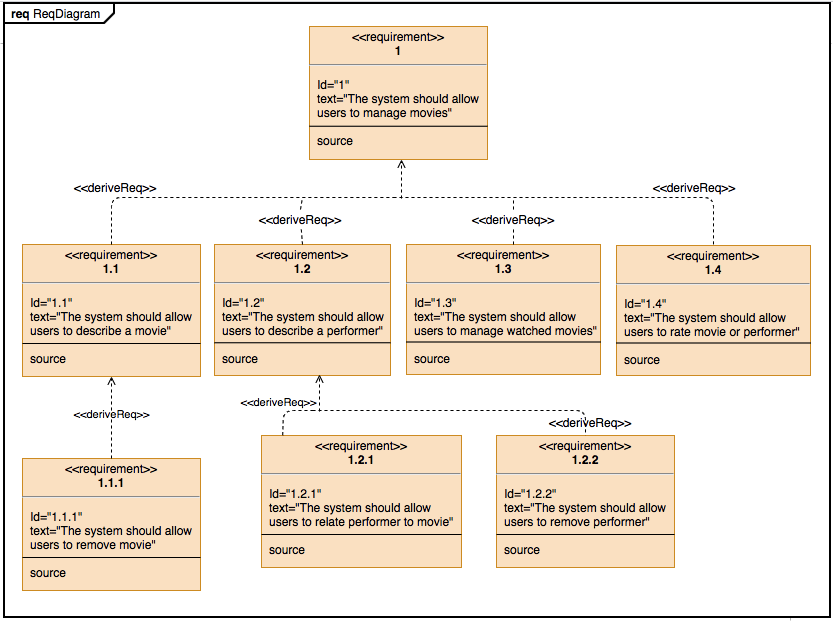
\includegraphics[scale=0.49]{../images/Ap1-req} 
\caption{Example of a SysML requirements diagram}
\label{fig:Ap1-req}
\end{figure}

%As presented in Figure~\ref{fig:Ap1-s2}, 
Then, the UML models of the SUT are built starting from the requirements models. During this process, the requirements should be traced to different parts of the models to point how each requirement is addressed by the models. In the provided approach, a set of modeling guidelines and validation rules should be defined for ensuring the quality of the resulting models. For this purpose, Object Constraint Language (OCL) is used. The aforementioned NoMagic’s MagicDraw tool has been used for editing the SysML and UML models and for running the validation rules. But in our implementation of the approach, we use the free online tool of the diagram software \textit{draw.io}\footnote{draw.io \url{https://drawio-app.com/}} via \textit{diagrams.net}\footnote{diagrams.net \url{https://www.diagrams.net/}} for this purpose.
\newpage
As the next step, a state machine model should be modeled from the requirements model, which is to be used as input for Qtronic, since the Qtronic tool expects the behavior of SUT in the form of state machines in order to be able to convert it into QML. %In the provided approach, the relationships between requirements and models are specified on several levels. For instance, non-leaf requirements are linked to state machine models, and leaf requirements in the requirements tree are linked to other UML elements to which they apply, e.g. transitions in a state machine or classes in a class diagram. As an exceptional situation, the top-level functional requirements are linked to use cases in the use case model of the SUT. \\
In \autoref{fig:Ap1-sm2}, we present an example for the requirement with the requirement id \enquote{1.4} from the requirements model presented in \autoref{fig:Ap1-req}.

\begin{figure} [H] 
\centering
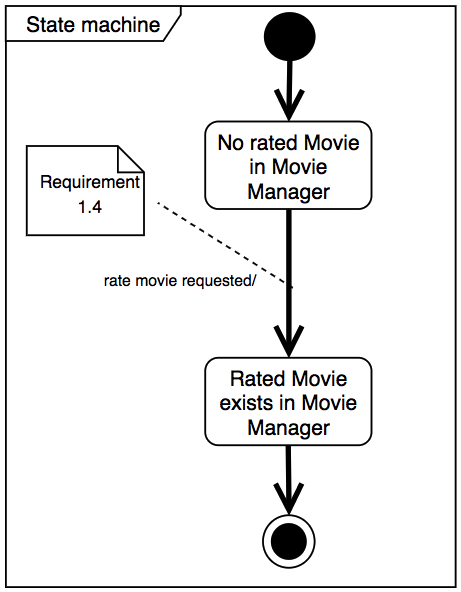
\includegraphics[scale=0.3]{../images/Ap1-sm2} 
\caption{Example of a UML state machine}
\label{fig:Ap1-sm2}
\end{figure}

But as already mentioned in the description of this approach in ~\autoref{subsec:DE1}, Qtronic is no longer available and therefore we can not apply the remaining steps, which are \textit{automatic test design and execution} and \textit{generation of test report}. As we could not find any information on how Qtronic generates tests, we can not provide any exemplarily test cases either. 




\section{Approach 2: Requirements Traceability in the Model-Based Testing Process}
\label{sec:AP2}

This section describes the approach presented in \textit{Requirements Traceability in the Model-Based Testing Process} \cite{Paper2}, and its application on Movie Manager. 

\subsection{Description}
\label{subsec:DE2}
This approach was presented in 2007 by Eddy Bernard and Bruno Legeard in \cite{Paper2} to automatically produce the traceability matrix from requirements to test cases, as part of the test generation process. Automatically generating the traceability matrix from requirements to test cases implies managing the links between the requirements specification, the model and the test cases. This approach focuses on this problem and is embedded in the \textit{LEIRIOS Test Designer} technology, which is named currently \textit{Smartesting}\footnote{Smartesting \url{https://www.smartesting.com/}} \cite{matera}. The approach tags the dynamic part of the UML model with the requirement identifiers and uses it to produce automatically both the test cases and the traceability matrix. 

First, the validation engineer constructs the model from a textual specification. The goal of this step is to translate the description of the features of the tested system into a precise UML model of the expected behavior \cite{LTG}. The LEIRIOS Test Designer approach uses a subset of the UML 2.0 language with class diagrams, instance diagrams, state machine diagrams, and OCL expressions. While the OCL expressions within the class diagram formally describe the expected behavior of operations of a class using preconditions and postconditions, the OCL expressions within the state machine formalize guards and effects of transitions between the states. 

Then, requirements traceability is managed by tagging manually the postconditions of the operations and the effects of the transitions in the UML model with the requirements. The format uses ad-hoc comment symbols to associate a requirement with an OCL statement which will be involved into a test target during the generation of the test cases. Once the model is reasonably trustworthy, the generation of tests is steered by the validation engineer on the basis of test selection criteria. Test selection criteria are supported by the LEIRIOS Test Designer tool to control the choice of tests from all the possible tests that can be derived from the behavior UML model \cite{LTG}, e.g. transition-based coverage, decision-based coverage, and data-oriented coverage. It is important to notice that all these test selection criteria are related to models and define how well the generated test suite covers the model \cite{LTG}. 

The test generation method is provided by the LEIRIOS Test Designer tool. It consists in testing all the possible behaviors of the specification operations, by traversing the states of the system. This strategy is controlled by the previously defined test selection criteria. 
\newpage
This method is performed as follows:
%
\begin{itemize}[noitemsep]
  \item [--]Partitioning of the model operation to generate all the possible expected behaviors,
  \item [--]Computation of variable domain boundaries from each behavior (called test targets),
   \item [--] Generation of test cases obtained, for each test targets, by traversing the underlying reachability graph of the model from the initial state to reach a state satisfying a test target.
\end{itemize}
Operations are the internal actions that modify the system state during the computation of user actions. They are called from the action part of transitions in the state machine and their meaning is defined by OCL postconditions in the class diagram \cite{LTG}. 

A test case reaches a target, which involves OCL statements tagged with one or several requirement identifiers. Then, LEIRIOS Test Designer makes it possible to match a test with requirements during the generation of the test cases. In LEIRIOS Test Designer, a general framework to convert the generated test cases into executable scripts is also provided. The test script pattern is a source code file in the target language with some tags indicating where sequences of operation invocations have to be inserted. A traceability matrix is obtained after the tests are executed. For each requirement, the matrix gives the list of needed test cases to test it. 

In \cite{Paper2}, this presented approach is implemented on a simplified version of a drink vending machine controller, which is SUT, with \enquote{Buy a drink} scenario to illustrate the test generation process with LEIRIOS Test Designer. After expected functional requirements of the SUT are listed, it is modeled via a \textit{class diagram}, an \textit{instance diagram} and a \textit{state machine}. Expected behaviors are specified by transitions (either external or internal) and those transitions are triggered by a \textit{user event}, a \textit{guard} and an \textit{effect}. Requirements traceability is managed by tagging the effect of each transition with requirement identifiers. This link between the model and the requirements is used by the LEIRIOS Test Designer tool to produce the traceability matrix between generated test cases and requirements. At the end, from the SUT model, 12 test targets are generated, one for each transition, and 12 test cases are generated. 

Unfortunately, the approach lacks the detailed explanation on how the test cases are generated and converted to executable test scripts via LEIRIOS Test Designer tool.




\subsection{Application}

In this part, we aim to to follow the same steps of the approach on our Movie Manager example as similar as possible. 

First, we get the informal requirements of the system under test. To do that, we create use case diagram of Movie Manager using draw.io tool as shown in \autoref{fig:Ap2-2}. Our use case scenario: \enquote{User manages movies and corresponding performer data of a movie collection}.

\begin{figure} [H] 
\centering
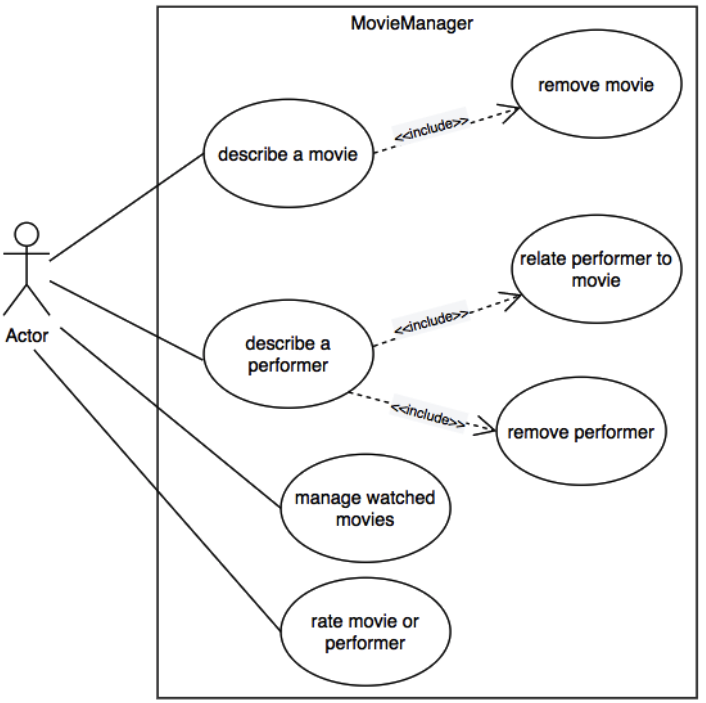
\includegraphics[scale=0.35]{../images/Ap2-2} 
\caption{Example for a use case diagram of Movie Manager}
\label{fig:Ap2-2}
\end{figure}

The system under test is the Movie Manager. To precisely define the expected functional requirements of the Movie Manager, a list of requirements including Req Identifier, Req Name, and Req description is defined as presented in \autoref{tab:MMreq}. For the requirements MM-2 and MM-7 we added some preconditions based on the Movie Manager \cite{MovieManager} to be able to apply the next steps of the approach within this section. 

\begin{table} [H] 
  \begin{center}
  \begin{small}
\caption{Movie Manager requirements}
\label{tab:MMreq}
\begin{tabular}{  m{1.3cm} | m{3.8cm} | m{8cm}  }
\hline
\textbf{Req. Id}& \textbf{Req. Name}&\textbf{Req. Description}   \\
\hline
MM-1& Describe\_Movie&The Movie Manager shall allow to describe a movie\\
\hline
MM-2&Remove\_Movie&The Movie Manager shall allow to remove movie. If the movie is linked with a performer, the user is warned by Movie Manager. The movie is removed from the database after user confirms.\\
\hline
MM-3&Describe\_Performer& The Movie Manager shall allow to describe a performer\\
\hline
MM-4&Relate\_Performer\_to\_Movie&The Movie Manager shall allow to relate performer to movie \\
\hline
MM-5&Remove\_Performer& The Movie Manager shall allow to remove performer\\
\hline
MM-6&Manage\_Watched\_Movies& The Movie Manager shall allow to manage watched movies\\
\hline
MM-7& Rate\_Movie\_or\_Performer& The Movie Manager shall allow to rate movie or performer. If the movie or performer does not exist, the user is warned by Movie Manager\\
\hline
\end{tabular}
\end{small}
 \end{center}
\end{table}

Then as an instance, we create the Movie Manager Class Diagram for the aforementioned requirements as presented in \autoref{fig:Ap2-class}.

\begin{figure} [H] 
\centering
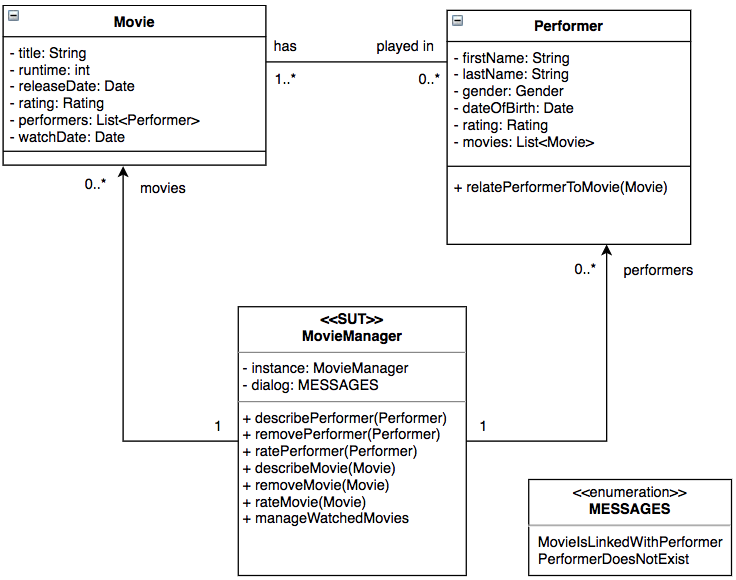
\includegraphics[scale=0.42]{../images/Ap2-class} 
\caption{Example for a class diagram of Movie Manager}
\label{fig:Ap2-class}
\end{figure}

The Movie Manager Class Diagram defines the data and the points of control and observation of the application under test. The enumeration \enquote{Messages} represents the possible message/warning to be displayed on the dialog window of the application. For our case, we considered only the messages like, \textit{movie is linked with performer} and \textit{performer does not exist}.

In addition to class diagram, an instance diagram and a state machine are also provided in the use case scenario of the provided approach. In the approach, the test generation method of LEIRIOS Test Designer consists in testing all the possible behaviors of the specification operations, by traversing the states of the system. But in our implementation, we have to skip this step since it is performed by the LEIRIOS Test Designer tool, which is called now Smartesting as already explained in ~\autoref{subsec:DE2}. We cannot use the tool right now, because it requires a scheduling even for the demo version. 

Therefore, we give only exemplarily two different internal activities specified according to the description in the article \cite{Paper2}, one for the user option \enquote{remove movie}, and other one for the user option \enquote{rate performer}, as shown in \autoref{tab:intact}. 

\begin{table} [H] 
	\begin{small}
  \begin{center}
  \begin{scriptsize}
\caption{Example of internal transitions}
\label{tab:intact}
\begin{tabular}{  m{3.3cm} | m{3.4cm} | m{6.4cm}  }
\hline
\textbf{Trigger/Label}& \textbf{Guard}&\textbf{Effect}   \\
\hline
removeMovie (movie)
\newline- Case movie is linked with a performer & Movie-$>$linked (m: movie $|$ m.linked=True) & MESSAGES\textbf{::} MovieIsLinkedWithPerformer \textbf{/*@REQ: MM-2@*/}\\
\hline
ratePerformer (performer)
\newline- Case performer does not exist & Performer-$>$exists (p: performer $|$ p.exists=False) & MESSAGES\textbf{::} PerformerDoesNotExist \textbf{/*@REQ: MM-7@*/ }\\
\hline
\end{tabular}
\end{scriptsize}
 \end{center}
\end{small}
\end{table}

These are the transitions, which are triggered by a user event, a guard and an effect. Requirements traceability is managed by tagging the effect of each transition with requirement identifiers. For example, the requirement MM-7 is used to annotate the effect in case of not existing performer. This is the link between the model and the requirement. \\
As last step, this link between the model and the requirements should be used by the LEIRIOS Test Designer tool to produce the traceability matrix between generated test cases and requirements. For each transition a test target and a test case should be via LEIRIOS Test Designer tool generated. Since we cannot use the tool, we generate the test cases as an example for both transitions manually. \autoref{tab:T1} and \autoref{tab:T2} presents these generated test cases for the two internal transitions showed in \autoref{tab:intact}.

\begin{table} [H] 
  \begin{center}
  \begin{small}
\caption{Test 1: Movie is linked with performer - Covered Requirements: MM-2}
\label{tab:T1}
\begin{tabular}{ m{0.8cm} | m{5cm} | m{7.3cm} }
\hline
\textbf{Step}& \textbf{Operation}&\textbf{Attributes Values}   \\
\hline
1 & MM2.removeMovie (movie)& MM2.display = MovieIsLinkedWithPerformer\\
\hline
\end{tabular}
\end{small}
 \end{center}
\end{table}
\begin{table} [H] 
\begin{center}
 \begin{small}
\caption{Test 2: Performer does not exist - Covered Requirements: MM-7}
\label{tab:T2}
\begin{tabular}{  m{0.8cm} | m{5cm} | m{7.3cm}  }
\hline
\textbf{Step}& \textbf{Operation}&\textbf{Attributes Values}   \\
\hline
1 & MM7.removePerformer (performer) & MM7.display = PerformerDoesNotExist\\
\hline
\end{tabular}
\end{small}
 \end{center}
\end{table}



\section{Comparison}
\label{sec:Compar}

In this section, we describe the special features, similarities and differences of each approaches.

Both approaches are very similar in terms of the way they use the information and of their steps. They both use informal requirements as input for their approaches, use system models for this purpose (UML models including OCL), and make use of requirements traceability for ensuring the quality of the generated test cases. They both offer tool support to generate tests automatically. \\
However, there are also differences between them. In the first approach, \cite{Paper1}, the informal requirements are analyzed and structured into requirements models and then OCL is used for verifying the quality of these requirements models.
In the second approach, \cite{Paper2}, the expected functional requirements of the system under test are derived from a use case scenario. The requirements traceability is managed by tagging manually the postconditions of the operations and the effects of the transitions in the UML model with the requirements via ad-hoc comment symbols in order to associate a requirement with an OCL statement which will be involved into a test target during the generation of the test cases. \\
Furthermore, the LEIRIOS Test Designer tool provided in the second approach does not offer a tool support for tracing-back requirements from tests to models, while the first approach supports it via the automatically generated test report by their provided tool, Qtronic.

\autoref{tab:TSM} presents the detailed comparison of both approaches as a synthesis matrix. In the first column, the number of the synthesis questions are presented. The synthesis questions are already documented in \autoref{sec:intruduction1.3}. Then, the second column presents the answers to these questions for approach 1, and the third column for approach 2. 

\newpage
\newgeometry{margin=1cm}
\begin{landscape} 
%\begin{scriptsize}
\begin{small}
\begin{longtable}{ p{0.5cm} | p{11cm} | p{11cm} }
\caption{Synthesis matrix}
\label{tab:TSM}
\\    %%%%<===
\hline
\textbf{No.} & \textbf{Approach 1: Tracing Requirements in a Model-Based Testing Approach}  & \textbf{Approach 2: Requirements Traceability in the Model- Based Testing Process} \\
\hline
1a) & - Informal requirements
\newline - Requirements models via requirements diagram of SysML
\newline - UML Models, e.g. class Diagram specifies a domain model, a behavioral model describes the behavior of the SUT using state machines, data models describe the message types exchanged between different domain entities, domain configuration models represents specific test configurations using object diagrams.
\newline - Generated tests and test report
 & - Informal requirements
\newline - UML Models (including OCL) e.g. Use case diagram, class diagram, enumeration diagram, instance diagram, state machine.
\newline - Links between the requirements and models
\newline - Test cases and test scripts
\newline - Traceability Matrix \\
\hline
1b) & Informal requirements are input for this approach.
\newline A set of modeling guidelines and validation rules should also be defined.
\newline In order to automatically transform UML models to the QML via the Qtronic tool, all requirements should have been linked to model elements and the models should have been validated.
\newline The desired coverage criteria used for test generation should be manually selected from the GUI of Qtronic.
\newline The presented approach is for functional requirements and it only supports online testing. & Informal requirements are input for this approach. 
\newline Uncontrollable or unobservable elements should not be modeled.\\
\hline
1c) & 1. The informal requirements are analyzed and structured into a requirements model using the requirements diagrams of the SysML.
\newline 2. SUT is specified using UML (including OCL) and several perspectives of the SUT are modeled, e.g. class diagram, behavioral model, data models, domain configuration models etc. 
\newline 3. A set of modeling guidelines and validation rules are defined using OCL. MagicDraw tool has been used for editing the SysML and UML models and for running the validation rules
\newline 4. The models used to specify the SUT are subsequently transformed into input for the automated test derivation tool Qtronic. 
\newline 5. At the end of each test run, an automatically generated test report will summarize the result of the testing process in terms of generated test cases, verdicts, coverage levels etc.
& 1. UML-Modelling of functional requirements of the application under test, e.g. class diagrams, instance diagrams, state machine diagrams  etc.
\newline2. Tagging manually the post-conditions of the operations and the effects of the transitions in the UML model with the requirements. The format uses ad-hoc comment symbols in order to associate a requirement with an OCL statement which will be involved into a test target during the generation of the test cases.
\newline3. Driving the test generation process in which the generation of tests is steered by the validation engineer on the basis of test selection criteria.
\newline4. Test generation method provided by the LEIRIOS Test Designer tool
\newline5. Executable test script generation which are converted from the generated test cases via LEIRIOS Test Designer. A test script pattern and a mapping table are to be defined by the test engineer.\\
\hline
2a) & Test generation, and tracing requirements to models, to test specification, and back to models again.& Test generation, and tracing requirements to test cases. \\
\hline
2b) & Product engineer, software engineer, requirement engineer and user of the provided tooll/tester.  & Validation engineer, software engineer, requirement engineer and user of the provided tool/tester. \\
\hline
2c) & Chapter 1: Software Requirements
\newline - Requirements Process
\newline - Requirements Analysis
\newline - Practical Considerations (e.g. Requirements Tracing)
\newline Chapter 4: Software Testing
\newline - Test Techniques (e.g. Model-Bases Testing Techniques)
\newline -  Software Testing Tools (e.g. Testing Tool Support and Categories of Tools)
\newline Chapter 9: Software Engineering Models and Methods 
\newline - Modeling
\newline - Types of Models
\newline - Analysis of Models (e.g. Traceability) & Chapter 1: Software Requirements 
\newline - Requirements Process (e.g. Process Actors)
\newline - Requirements Analysis
\newline - Practical Considerations (e.g. Requirements Tracing)
\newline Chapter 4: Software Testing
\newline - Test Techniques (e.g. Model-Bases Testing Techniques)
\newline -  Software Testing Tools (e.g. Testing Tool Support and Categories of Tools)
\newline Chapter 9: Software Engineering Models and Methods 
\newline - Modeling
\newline - Types of Models
\newline - Analysis of Models (e.g. Traceability) \\  
\hline
3a) & The NoMagic’s MagicDraw has been used for editing the SysML and UML models and for running the validation rules. \newline Conformiq’s Qtronic tool is provided for the automated test derivation and test report generation. Only online testing mode of Qtronic is used to generate tests. & LEIRIOS Test Designer tool is provided to generate test cases and to produce the traceability matrix between generated test cases and requirements. The tool is used in the test and test script generation processes.\\
\hline
3b) & The creation of the models is not automated and the desired coverage criteria used for test generation should be manually selected from the GUI of Qtronic. Tests and test reports are automatically generated by the provided tool, Qtronic. &Requirements traceability is managed by tagging manually the postconditions of the operations and the effects of the transitions in the UML model with the requirements via ad-hoc comment symbols. Tests are automatically generated by the provided tool, LEIRIOS.\\
\hline
4a) & Approach does not present an evaluation. Only validation rules have been defined and implemented for both requirements models and for SMs for checking different quality metrics of the resulting models before proceeding to the test derivation phase.
\newline For the description of the approach, only small examples from a telecommunications case study are provided. & Approach does not present an evaluation. Only for a simpler description, the approach is implemented on a simplified version of a drink vending machine controller.\\
\hline
4b) & Since the approach does not offer any evaluation, only the benefits and shortcomings of the approach have been shared as below:
\newline - The approach provides a solution for tracing only functional requirements and supports only online testing.
\newline - The approach provided automation of the transitions between the phases of the process, allowing to have a fast feed-back loop for testing and debugging specifications or the implementation of the SUT.
\newline - Many errors have been detected in the early stages of the process, when the system models have been created. The errors were caused mainly by omissions in the models and by misinterpreting the requirements.
\newline - Since the approach is fully automated, the effort in updating the models and performing the testing again was diminished.
 & Since the approach does not offer any evaluation, only the benefits and shortcomings of the approach have been shared as below:
 \newline - Automatically produced traceability matrix leads to several advantages in the software testing process, e.g. it gives a clear functional coverage metrics to the generated test cases, enables to improve the model or test generation strategies, and gives valuable feed-back on the requirements.
 \newline - There is no tool support for tracing-back requirements from tests to models.\\
\hline
\end{longtable}
\end{small}
%\end{scriptsize}
\end{landscape} 
\restoregeometry


\newpage
\section{Conclusion}
\label{sec:Conc} 
This chapter presents two approaches for the testing with system models. Both approaches, \cite{Paper1} and \cite{Paper2}, use requirements traceability in their model-based test generation processes and provide a tool support to generate tests automatically. 

The literature research showed us that the for this topic relevant articles are mostly published between 2000-2009. Although there are a lot of articles which provide approaches based on the links (traces) between requirements and test cases, only a few of them are using system models. Therefore, it is important to differentiate the system model and test model with respect to the model-based testing. However, based on our research, we could not find a sharp difference between the two. Our conclusion is that test models are developed solely for testing while system models can be primarily developed for system development and then used for testing as well. Moreover, with this literature study, we came to the conclusion that it is laborious to find relevant articles with keyword-based search method, because requirements traceability and model-based testing are very comprehensive topics in Software Engineering. 

The first approach studied in this chapter, \cite{Paper1}, describes the MBT process in more detail than the second approach \cite{Paper2} does. But \cite{Paper2} presents a more detailed use case example with more visuals which enables us to understand the steps of the testing process better. However, both approaches lack the detailed explanation on how the test cases are generated via the provided test generation tools. For the generation of test cases, \cite{Paper1} provided Conformiq's Qtronic tool, which is unfortunately not existing anymore, and \cite{Paper2} provided the LEIRIOS Test Designer tool, which is named currently Smartesting. Therefore, we could not find the necessary information on how these tools implement the test generation step in practice. Unfortunately, no evaluation was offered for either approach. All of this makes it difficult for us to make an accurate assessment between these two tools/approaches. In our opinion, if we had to choose one of this approaches, it would make more sense to choose the second approach \cite{Paper2}, as LEIRIOS Test Designer tool (Smartesting) is still on the market. It has probably evolved over the ten years as well.

Finally, both approaches presented in this chapter showed us that testing with system models enables to increase the possibility of finding errors, reduce the testing time, and improve the test quality using requirements traceability.

\chapter{Testing functional and nonfunctional requirements in User Requirements Notation}\label{sec:topic_8}

%
% Hinweis:
%
% Die Tabellenanordnung, etc muss noch überprüft werden.
% Teilweise sind Figures auf der falschen Seite, trotz [h!]
%

\chapter{Testing Non-Functional Requirements with Risk Analysis}\label{sec:topic_9}

% Andre Meyering

\section{Introduction}

In contrast to functional requirements (FRs) that describe the program's functionality, i.e. how it processes data and user input, non-functional requirements (NFRs) describe constraints that the program must adhere to~\cite{SWEBOK}.
Parts of NFRs are performance and security requirements which can directly affect the end-user but also maintainability requirements which are more important to development teams.
While there are lot of resources about testing FRs in the form of unit-, integration- and end-to-end-tests, no common testing framework or guidance for testing NFRs exists.

For this reason, we look into two approaches \cite{ZouPavlovski2008} and \cite{Lagerstedt2014}.
While \cite{ZouPavlovski2008} was given in advance by the advisors of the seminar, \cite{Lagerstedt2014} was found through a literature search, which is described in \autoref{sec:9_literature}.
Each approach will be described and applied to an example in the form of movie management software in the respective \autoref{sec:9_approach_1} and \autoref{sec:9_approach_2}. 

Both approaches are compared in \autoref{sec:9_comparison} by using a synthesis matrix. We will look at which NFRs are covered and how they are tested.
The results of this chapter will be summarized and concluded in \autoref{sec:9_conclusion}.

Please refer to the glossary for the following terms used throughout this chapter:
test case, use case, NFR.



%%%%%%%%%%%%%%%%%%%%%%%%%%%%%%%%%%%%%%%%%%%%%%%%%%%%%%%%%%%%%%%%%%%%%%%%%%%%%%
%%%%%%%%%%%%%%%%%%%%%%%%%%%%%%%%%%%%%%%%%%%%%%%%%%%%%%%%%%%%%%%%%%%%%%%%%%%%%%

\section{Literature search} \label{sec:9_literature}

The starting point for the literature search was the paper given to us~\cite{ZouPavlovski2008}.
Based on this paper, we formulated the central research question: 

\hspace*{0.5cm}\enquote{\textit{Which approaches for testing non-functional requirements systematically\newline \hspace*{0.7cm}with risk analysis exist?}}.

We focused on finding articles that covered the three most important keywords and phrases for the topic: \textit{testing}, \textit{non-functional requirements} and \textit{risk analysis}.
A quick search using these three phrases resulted in IEEE Xplore having the most promising results, whereas ACM\footnote{\url{https://dl.acm.org/}} only showed a few.
Because the given article \cite{ZouPavlovski2008} can also be found on IEEE~Xplore\footnote{\url{https://ieeexplore.ieee.org/Xplore/home.jsp}}, we focused our search onto that site but still looked at ACM.

To be able to evaluate the relevance of papers found during the literature search, we defined three relevance criteria:

\begin{enumerate}
	\item Does the article cover non-functional requirements? They must not only  be mentioned as a side note next to functional requirements.
	\item Does the article combine risk analysis with tests?
	\item Does the article cover \textit{testing} of non-functional requirements?
\end{enumerate}

Even though these relevance criteria basically only cover the research question, they filter out most non-relevant papers as we will see later on.

% https://ieeexplore.ieee.org/document/4578345
The search was carried out by using forward and backward snowballing as well as by using search terms with combinatorial modifiers.
Only two papers reference \cite{ZouPavlovski2008} according to its IEEE~Xplore site, both of which cover functional but not non-functional requirements.
The paper itself references 23 papers.
Of those papers, only few covered the first criterion and none covered the third criterion.
\cite{ZouPavlovski2008} itself does not cover risk analysis as a main research topic but only covers it in a side note (see \autoref{sec:9_approach_1}).
This is why search-term based search was performed using the key terms: non-functional requirements, testing and risk analysis.

\autoref{tbl:search_topic_9_andre} lists an excerpt of the term-based search.
Listed are only those searches that returned promising results or highlight issues I encountered during the search.
It can be seen that, if all keywords are combined using the \texttt{AND} operator with the default restrictions, no relevant results were returned.
After a feedback from one advisor, the search was changed so that \enquote{non-functional requirements} and \enquote{testing} were expected in the paper's abstract, but \enquote{risk analysis} was searched for in \textit{all} metadata including the full text.
It turned out that no papers were found which mentioned risk analysis as well as the other two keywords in their abstract.

We also discovered that the spelling of the term \enquote{non-functional} had a huge impact on the results returned by IEEE~Xplore.

\begin{small}
	\centering
	\begin{longtable}[bth]{p{0.08\textwidth}|c|p{0.58\textwidth}|p{0.12\textwidth}}
		\caption{Term based search results}
		\label{tbl:search_topic_9_andre}
		\setlength{\tabcolsep}{1em}\\    %%%%<===
		\hline
		\textbf{Source} & \textbf{Date} & \textbf{Search query and restrictions} & \textbf{\#Results (relevant)} \\
		
		\hline
		IEEE Xplore & 2020-11-11 & \texttt{\enquote{{}non-functional requirements}{} AND testing AND \enquote{{}risk analysis}{}} & 3 (0) \\
		
		\hline
		IEEE Xplore & 2020-11-11 & \texttt{non-functional requirements AND testing AND risk analysis} & 12 (0) \\
		
		\hline
		IEEE Xplore & 2020-11-11 & \texttt{risk AND \enquote{non-functional} and test} & 23 (2) \\
		
		\hline
		IEEE Xplore & 2020-11-29 & \texttt{((\enquote{{}Abstract}{}:nonfunctional requirements) AND \enquote{{}Abstract}{}:Test) AND \enquote{Full Text \& Metadata}:\enquote{{}risk analysis}{})} & 2 (1) \\
		
		\hline
		IEEE Xplore & 2020-11-29 & \texttt{((\enquote{{}Abstract}{}:non-functional requirements) AND \enquote{{}Abstract}{}:Test) AND \enquote{Full Text \& Metadata}:\enquote{{}risk analysis}{})} & 3 (0) \\

		\hline
		ACM & 2020-11-29 & \texttt{[Abstract: \enquote{{}risk}{}] AND [Abstract: test*] AND [Abstract: \enquote{{}non functional}{}]} & 4 (1) \\
		
		\hline
		ACM & 2020-11-29 & \texttt{[Abstract: test] AND [Abstract: \enquote{{}non functional}{}] AND [[Full Text: \enquote{{}risk analysis}{}] OR [Full Text: \enquote{{}risk}{}]]} & 20 (1) \\
		\hline
	\end{longtable}
\end{small}

After this initial search, the resulting papers were evaluated and one paper was chosen. The papers to chose from included:

\begin{itemize}
	\item \enquote{Scenario-Based Assessment of non-functional Requirements } \cite{Andre_Search_1}
	\item \enquote{Alignment of requirements specification and testing: A systematic mapping study} \cite{Andre_Search_2}
	\item \enquote{Using Automated Tests for Communicating and Verifying Non-functional Requirements} \cite{Lagerstedt2014}
\end{itemize}


\textit{Scenario-Based Assessment of non-functional Requirements} covers all three criteria we defined at the start of our search. However, it limits itself to complex socio-technical systems and only looks at one non-functional requirement, which is the system's performance.  It limits itself to the evaluation of the reliability of certain aspects of software which interacts with humans to calculate the risk of human errors occurring.
This is done by implementing scenarios--hence the title \enquote{scenario-based assessment}. The testing aspect of this paper is limited to human-interactions whose risks are evaluated. If scenarios fail this risk assessment, then so will the test.

\textit{Alignment of requirements specification and testing: A systematic mapping study} is about papers that cover non-functional requirements. It is a study about such papers and lists approaches that are used to test NFRs. Some of which are mentioned in other chapters of this paper. However, none cover risk analysis. The paper itself does not give much insight into testing non-functional requirements itself.

The chosen article which we will further evaluate in the following sections is \textit{Using Automated Tests for Communicating and Verifying Non-functional Requirements}. It covers the non-functional requirement \enquote{maintainability} and how it can be tested. It further explains it by using practical examples.
However, the chosen paper does not cover risk-analysis. Since no paper could be found that covers all criteria, we were advised to focus on the testing of non-functional requirements and leave out risk-analysis.


%%%%%%%%%%%%%%%%%%%%%%%%%%%%%%%%%%%%%%%%%%%%%%%%%%%%%%%%%%%%%%%%%%%%%%%%%%%%%%
%%%%%%%%%%%%%%%%%%%%%%%%%%%%%%%%%%%%%%%%%%%%%%%%%%%%%%%%%%%%%%%%%%%%%%%%%%%%%%


\section{Approach 1: Control Cases during the Software Development Life-Cycle } \label{sec:9_approach_1}


\subsection{Description}

In their paper \enquote{Control Cases during the Software Development Life-Cycle}~\cite{ZouPavlovski2008}, J. Zou und C. J. Pavlovski based their work on so called  \enquote{control cases} and \enquote{operating conditions} as tools for modeling and controlling NFRs.
\newpage
\enquote{Control cases} are used as a format to communicate and discuss NFRs between management, requirement engineers, developers, and system users and to define qualitative attributes of the system.

Their work focuses on determining and revealing problems early on, for example bad performance or security risks.
The classic software development life cycle often focuses on these topics too late or not at all.
However, control cases require NFRs to be defined first.
To define them, the paper starts by introducing operating conditions.
Operating conditions model constraints that apply to the system or a specific use case. These constraints are then used to model NFRs, hence the operating condition can be seen as a high level view on NFRs.
Defining such constraints that apply to a certain use case is left to the reader or rather is mentioned as a step of the business process modeling.

Operating conditions can belong to one or more use cases and are not unique to a specific one. Conditions such as \enquote{Transaction Volume Condition: $>$400 concurrent users} can be applied to different use cases~\cite{ZouPavlovski2008} and model exactly that: a condition under which the use case operates.

Control cases--as the name suggests--control the operating conditions and can be used to ensure that they are complied to.
This makes it possible to mitigate business risks which may affect the business if the operating condition and its constraints are violated.
Their paper visualizes the connection between these artifacts using an UML diagram, which can be seen in \autoref{fig:topic_9_appraoch_1_use_case} below.

\begin{figure}[htbp]
	\centering
	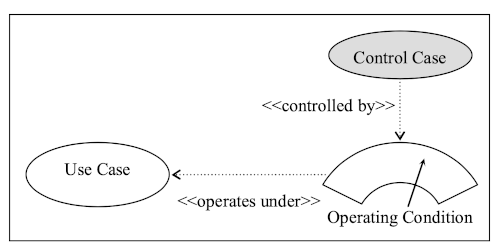
\includegraphics[width=0.4\textwidth]{../images/topic_9_approach_1_1.png}
	\caption{Association in Use Cases Modelling~\cite{ZouPavlovski2008}}
	\label{fig:topic_9_appraoch_1_use_case}
\end{figure}

The paper creates such a control case by introducing a fictional example of a traveling agent.
All of the previously mentioned artifacts are created during the \enquote{Business Process Modeling} and are refined throughout the software development life cycle.
This means that operating conditions and control cases are defined together with use cases and can be incorporated together in a use case model.
The paper does this for their fictional example which can be seen in \autoref{fig:topic_9_appraoch_1_2}. 

\begin{figure}[h!]
	\centering
	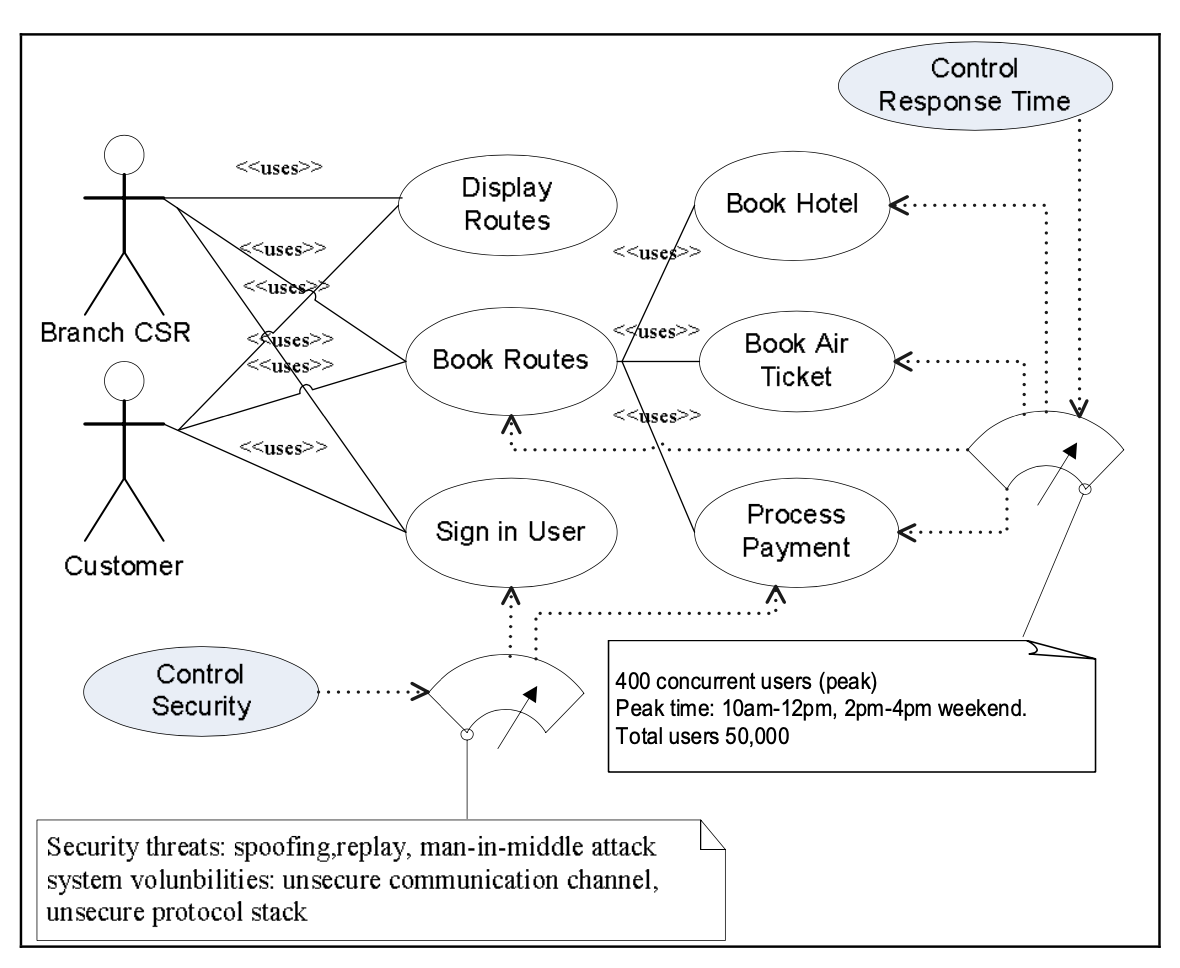
\includegraphics[width=0.65\textwidth]{../images/topic_9_approach_1_2.png}
	\caption{Use Case Model with Control Cases~\cite{ZouPavlovski2008}}
	\label{fig:topic_9_appraoch_1_2}
\end{figure}

In this graphic, control cases are visualized as shaded ellipses and operating conditions as speedometers, though unspecified by the paper. 
This graphic also emphasizes that operating conditions are not bound to one specific use case but can be applied to different ones.
And the control case is specific to one operating condition.


The reader is guided through all steps of the software development life cycle, so that a control case can be defined which is then used as the basis for a test case. Because the control case is associated to an operating condition, the test case is associated to it transitively as well.
The test case exists to verify that the controls put in place to manage the operating condition are effective.
\newpage
The paper does not give a detailed instruction how to model test cases. It only instructs testers to simulate the operating condition, for example by creating a huge work load on the server.
With this simulation relevant metrics can be extracted that are used to verify the test case.



\subsection{Application}

J. Zou und C. J. Pavlovski focus on creating control cases. This is done for the movie manager example.

We first define one goal of our software:
it must contain a movie list view that has smooth scrolling and can handle a large amount of movies.
This also defines a constraint and therefore our operating condition: we must operate a smooth list view.
If this cannot be accomplished an associated risk may affect the business. The control case bundles all of this in a matrix which is defined as in \autoref{tbl:topic_9_approach_1} on \autopageref{tbl:topic_9_approach_1}.

Based on this control case, developers can start to implement the software. During
testing stage, functional requirements can be tested by basing them on use cases. Non-functional requirements, on the other hand, can be tested by creating tests from control cases.
The tester needs to simulate the operating condition.
In our example above, that would mean to simulate the scrolling condition by creating a huge list of movies.
The steps that must be executed for the test are combined into a test case , such as \autoref{tbl:topic_9_test_case} on \autopageref{tbl:topic_9_test_case}.

By determining the operating condition that is associated to a use case, we were able to create a control case that reflects the NFRs.
Based on the operating condition, we then created a test case that checks if the controls put in place by the control cases are enough to mitigate the business risk.
Following this pattern, tests for non-functional requirements can be created systematically step by step.

%\clearpage

\begin{table}[p!]
	\centering
	\caption{Control Case for Approach 1 of Topic 9}
	\label{tbl:topic_9_approach_1}
	\begin{tabular}{p{0.95\textwidth}}\hline
		\textbf{Control Case}: Performance of the movie list view \\ 
		\hline
		\textbf{Control Case ID}: CC-001 \\
		\hline
		\textbf{Operating Condition}: Scrolling Speed Condition \\
		\hline
		\textbf{Description}: The control case describes the \enquote{smoothness} while scrolling through the movie list view. Scrolling must be smooth. If it is not then users may assume bad performance. \\
		\hline
		\textbf{NFR Category}: Performance and Capacity\\
		\hline
		\textbf{Associated Use Cases}: Show movies in list view \\
		\hline
		\textbf{Technical Constraints}: GUI Framework, Operating System (e.g. 32bit system only allows addressing of 4GB main memory) \\
		\hline
		\textbf{Vulnerability}: \newline Unknown number of movies. Users may only have a few or thousands of movies.
		Analyzing movies (or doing other work) must not lead to the movie list view being unresponsive. Having a lot of movies must not make the program run out of memory. \\
		\hline
		\textbf{Threat Source}: None (local software used by one user) \\
		\hline
		\textbf{Operating Condition}: There may be tens of thousands of movies. Assuming that each movie object has a size of 600kB (only meta data and a small thumbnail), loading 20,000 movies would lead up to 12GB of memory usage\tablefootnote{From personal experience by maintaining a media manager. Users regularly report more than 10,000 movies in their database.}. All movies must be represented in a list view.\\
		\hline
		\textbf{Business Risk}:\newline If scrolling is not smooth, the user may switch to other software or leave a bad rating. \\
		\hline
		\textbf{Probability}: medium (likely few users are affected) \\
		\hline
		\textbf{Risk Estimation}: \newline
		low (users with huge databases may accept higher load times or sluggishness in the UI) \\
		\hline
		\textbf{Control}: 
		\begin{enumerate}
			\item Only load visible movies into main memory. Use \enquote{infinite scrolling} techniques. Remove those movies from main memory that are not visible to the user.
			\item Only load the title into main memory. Load other details only if required. This reduces the memory footprint.
		\end{enumerate} \\
		\hline
	\end{tabular}
\end{table}


%
% ACHTUNG
%
% Bitte darauf achten, dass diese Tabelle auch bei Ansatz 1 landet und
% nicht bei Ansatz 2, wie es bei mir der Fall war.
%
\begin{table}[h!]
	\centering
	\caption{Test Case for the movie manager example of topic 9, approach 1}
	\label{tbl:topic_9_test_case}
	\begin{tabular}{p{0.95\textwidth}}\hline
		\textbf{Associated Control Case ID:} CC-001\\
		\hline
		\textbf{Test Objectives:} \newline Verify that the movie list view has no visible hiccups when scrolling through the list of movies. \\
		\hline
		\textbf{Preconditions:} Movie manager is up and running.\\
		\hline
		\textbf{Test Steps:} \begin{enumerate}
			\item Create 20.000 movies and load them into the movie manager
			\item Open the movie list view
			\item Scroll through the list of movies
		\end{enumerate} \\
		\hline
		\textbf{Expected Result:} \begin{enumerate}
			\item The end of the list view is reached.
			\item No hiccups while scrolling were visible, i.e. no \enquote{sluggishness}.
		\end{enumerate} \\
		\hline
		\textbf{Notes:} \newline
		The test must be performed on a system that has at most 8 GB of RAM to reflect common end-user hardware. \\
		\hline
		\textbf{Test Result:} Pass / Fail \\
		\hline
										
	\end{tabular}
\end{table}

%%%%%%%%%%%%%%%%%%%%%%%%%%%%%%%%%%%%%%%%%%%%%%%%%%%%%%%%%%%%%%%%%%%%%%%%%%%%%%
%%%%%%%%%%%%%%%%%%%%%%%%%%%%%%%%%%%%%%%%%%%%%%%%%%%%%%%%%%%%%%%%%%%%%%%%%%%%%%
\newpage

\section{Approach 2: Using Automated Tests for Communicating and Verifying Non-functional Requirements} \label{sec:9_approach_2}

\subsection{Description}

In \enquote{Using Automated Tests for Communicating and Verifying Non-functional Requirements}~\cite{Lagerstedt2014}, Robert Lagerstedt describes how testing NFRs can be automated by introducing a tool-based approach.
The author only looks at NFRs in regards to software architecture which affects code quality in the sense of maintainability and security.

By looking at software architecture aspects as NFRs, Lagerstedt describes how software may be written by listing some architectural requirements.
It should not have dependencies from lower code components into higher but only vice versa.
Certain functions must not be called from some components to ensure encapsulation. Some functions may be blacklisted due to security concerns.
All of these requirements are part of the software architecture and therefore a huge part of software quality and maintainability~\cite{Lagerstedt2014}.

These NFRs must be communicated to developers. According to Lagerstedt, this is done by guidelines written by software architects.
The compliance of these guidelines is often verified by different reports. These reports may be written for each code change as part of a code review or by other teams.
Lagerstedt visualizes this in a simple UML diagram as can be seen in
\autoref{fig:topic_9_approach_2_1}.
The graphic uses a rather high distance between the developer and the compliance report on purpose to symbolize that the two are asynchronous, this means that the report is not automated and feedback reaches the developer not immediately.

\begin{figure}[htbp]
	\centering
	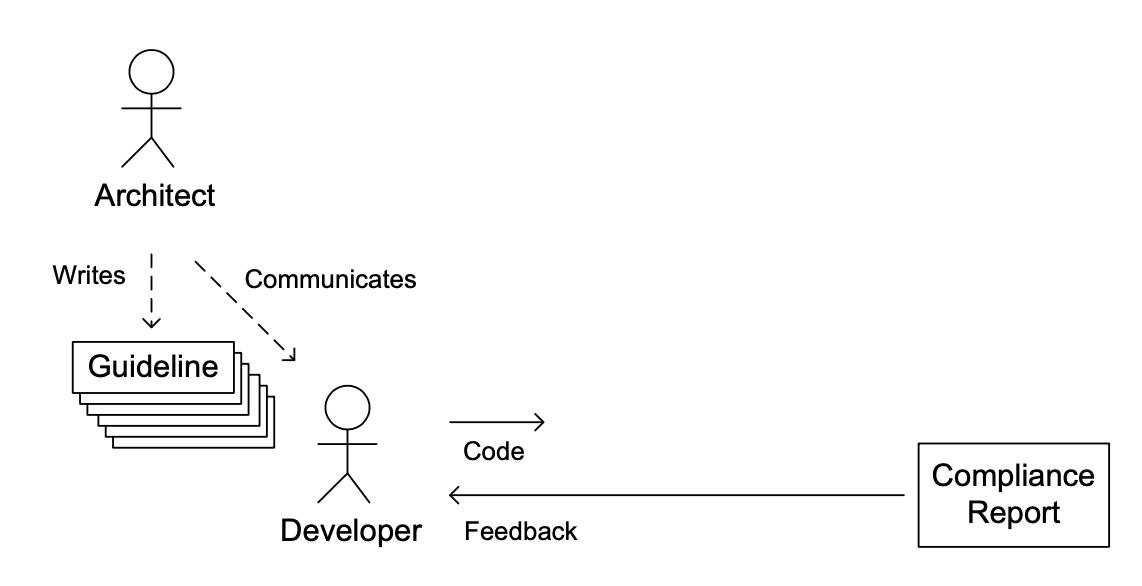
\includegraphics[width=0.6\textwidth]{../images/topic_9_approach_2_1.png}
	\caption{The common way of communicating architectural requirements~\cite{Lagerstedt2014}}
	\label{fig:topic_9_approach_2_1}
\end{figure}

This way of communicating guidelines is not very cost-efficient.
Every developer has to read and understand the guidelines. Developers must be re-trained when changes are made or if too many guidelines violations occur, because they have been forgotten.
This is quite time consuming and prone to error.  Creating reports about guideline compliance is time consuming as well.
Furthermore, while code review should be performed for all code changes, mistakes may slip through.

That is why the author proposes automated testing of software architecture NFRs.
This allows a fast tool-based feedback loop in which the developer gets a code review that can be incorporated without other developers having to look out for violations of guidelines.
On top of that, by having this tight feedback loop, developers can learn the guidelines in an iterative way.
Little to no training is required, which saves time to make new guidelines known to all developers.

The guidelines are written as tests. These tests can be included in existing static code analysis tools such as linters and other code checkers. Developers can see the results of such tools.
Furthermore guidelines are communicated to the developer in case of a test failure.
Lagerstedt uses \autoref{fig:topic_9_approach_2_2} to visualize this approach.
Developers get feedback through different tools that the architect extends. Tools such as the editor, compiler or static analysis tools.

\begin{figure}[htbp]
	\centering
	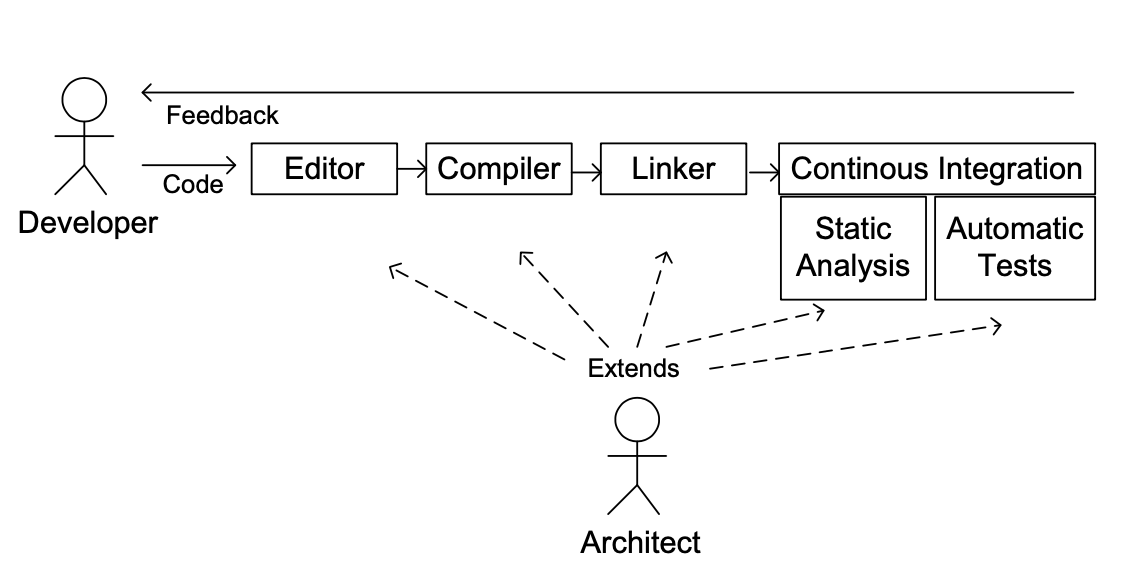
\includegraphics[width=0.7\textwidth]{../images/topic_9_approach_2_2.png}
	\caption{Suggested solution of communicating requirements~\cite{Lagerstedt2014}}
	\label{fig:topic_9_approach_2_2}
\end{figure}
\newpage
According to Lagerstedt's personal experience, a tool based approach is superior to a guideline-only one.
Productivity is increased while the time spent on communicating architectural guidelines is decreased.
The number of non-compliant code is lower for the tool-based approach than for using guidelines and reports only.


\subsection{Application}

The paper works with architectural NFRs but does not explain how those can be modeled.
To be able to apply the approach, we introduce another system function to the movie manager example that is listed in \autoref{tbl:topic_9_application_approach_2}.
This system function and the following NFRs are based on personal experience in maintaining an open-source media manager.

\begin{table}[h!]
	\centering
	\caption{New system function for application of approach 2 of topic 9}
	\label{tbl:topic_9_application_approach_2}
	\begin{tabular}{r|p{0.7\textwidth}}
		\hline
		\textbf{Name}          & Export the movie to HTML \\ \hline
		\textbf{Description}   & An existing movie is exported to a single HTML file which can be viewed in any modern web browser \\ \hline
		\textbf{Precondition}  & Movie exists \\ \hline
		\textbf{Input}         & Movie details \\ \hline
		\textbf{Postcondition} & HTML file exists with the movie's contents \\ \hline
		\textbf{Output}        & HTML file \\ \hline
	\end{tabular}
\end{table}

In \autoref{tbl:topic_9_approach_2_nfr} on \autopageref{tbl:topic_9_approach_2_nfr}, two NFRs are listed which were created for the system function in \autoref{tbl:topic_9_application_approach_2}. 
These two NFRs are based on personal experience.
Both are transformed into pseudo code so that the NFRs can be executed automatically as part of the code review.

While these two NFRs can be written as guidelines, especially point two may be violated and may slip through code review. Violating point two may result in security issues or at least in unexpected behavior if the HTML contains unescaped characters.
\newpage
\begin{longtable}{p{0.05\textwidth}|p{0.24\textwidth}|p{0.65\textwidth}}
	\caption{NFRs for the application of approach 2 of topic 9}
	\label{tbl:topic_9_approach_2_nfr}
	\setlength{\tabcolsep}{1em} \\
	\hline    %%%%<===
	\textbf{No.} & \textbf{NFR} & \textbf{Explanation} \\
	\hline
	1 & IMDb IDs are encapsulated in a class &
	All IMDb IDs have a certain format. They start with the string \enquote{tt} and end with 7-8 numbers. The ID must be validated which cannot be ensured by using a simple string. This is why an encapsulation in a class is required.
	
	Furthermore the programming language's type system can help to identify conversion bugs as well.
	\newline \newline \textit{Implementation in pseudo code}
	\begin{lstlisting}
for each $variable in $source:
 if $variable.startsWith("imdb") then
  if typeof($variable) != "ImdbId" then
   throw new Exception("Wrong class")
	\end{lstlisting}\\
	\hline
	
	2 & Exported strings are escaped &
	This is a security concern and can be implemented in different ways. We assume that an HTML-exporter was created which takes a movie object as an argument.
	This object may contain texts which contain HTML elements themselves.
	These elements need to be escaped. To ensure this NFR, all strings must be run through a certain function which escapes strings.
	
	Because this may be missed by the developer, a new string-subclass is introduced which escapes its input automatically, e.g. \texttt{EscapedString}.
	Only this string class may be used in the HTML exporter.
	\newline \newline \textit{Implementation in pseudo code}
	
	\begin{lstlisting}
for each $functionCall in $HTMLExporter:
 if $functionCall == "writeText" then
  $arg = argument of($functionCall);
  if typeof($arg) != "EscapedString" then
   throw new Exception("Wrong class")
	\end{lstlisting}

\textit{Note:} We assume that \texttt{writeText} is a method of a generic HTML-class which the HTML-exporter uses itself. We assume that the method cannot be changed to accept another argument type. Otherwise the language's type checker could already be able to find this issue.\\

\hline
\end{longtable}


%%%%%%%%%%%%%%%%%%%%%%%%%%%%%%%%%%%%%%%%%%%%%%%%%%%%%%%%%%%%%%%%%%%%%%%%%%%%%%
%%%%%%%%%%%%%%%%%%%%%%%%%%%%%%%%%%%%%%%%%%%%%%%%%%%%%%%%%%%%%%%%%%%%%%%%%%%%%%
%\clearpage
\section{Comparison} \label{sec:9_comparison}

For an improved comparison of these two approaches, a synthesis matrix is provided which references the questions from \autoref{sec:intruduction1.3}:

%\begin{enumerate}
%	\item Description of the approach (What does the approach do?)
%	\begin{enumerate}
%		\item Which artifacts and relations between artifacts are used in this approach? Which artifacts are created in the course of the approach? How are the artifacts characterized?
%		\item What is required and/or input for the application of the approach?
%		\item Which steps does the approach consist of? Which information is used in which step and how? What are the results of the individual steps?
%	\end{enumerate}
%	\item Benefits of the approach (Whom does the approach help and how?)
%	\begin{enumerate}
%		\item Which usage scenarios are supported by the approach?
%		\item Which stakeholders are supported by the usage scenarios?
%		\item Which knowledge areas from SWEBOK can be assigned to the usage scenarios?
%	\end{enumerate}
%	\item Tool support for the approach (What tool support is available?)
%	\begin{enumerate}
%		\item What kind of tool support is provided for the approach?
%		\item Which steps of the approach are automated by a tool? Which steps are supported by a tool, but still have to be executed manually? Which steps are not supported by a tool?
%	\end{enumerate}
%	\item Quality of the approach (How well does the approach work?)
%	\begin{enumerate}
%		\item How was the approach evaluated?
%		\item What are the (main) results of the evaluation?
%	\end{enumerate}
%\end{enumerate}

\begin{small}
\begin{longtable}[h]{p{0.02\linewidth}|p{0.455\linewidth}|p{0.455\linewidth}}
	\hline
	\textbf{No.} & \textbf{Approach 1 \cite{ZouPavlovski2008}} & \textbf{Approach 2 \cite{Lagerstedt2014}} \\
	\hline
	1a) & 
	Operating conditions are formed that work under specific use cases.
	These, on the other, hand are controlled by control cases and can be operated under them.
	Control cases describe the business risks in case that the operating condition cannot be fulfilled.
	Because use cases and control cases are tightly connected to each other, they can be modeled in one consolidated model.
	& 
	
	Coding guidelines are written and transformed into tests that can be used by tools in code review.
	These point out issues that the developer can fix.
	Guidelines are characterized by the fact that they describe the code architecture.
	\\
	\hline
	1b) & 
	There are no preconditions because we start defining control cases at the beginning of the software development process, for example at the \enquote{Business Process Modelling}-step.
	
	&
	The guidelines cover code architecture. They must be transformable into automated tests (e.g. by a static code analyzer).
	
	\\
	\hline
	
	1c) &
	Preconditions/Constraints must be extracted from which NFRs are created, e.g. performance or security constraints.
	These constraints are modeled by operating conditions for which control cases are created.
	Their purpose is to mitigate business risk which is essentially the failure to fulfill the operating condition.
	For each control case a test case is added that checks if the controls put in place by the control case are effective.
	The test case basically recreates the operating condition, for example by using stress testing.
	
	&
	Code guidelines such as naming conventions or prohibited function-calls are defined.
	These are transformed into automated tests that can be executed by the developer (i.e. a tool based approach).
	The exact process is not explained and it is left to the reader how this may be implemented.
	It is only pointed out that existing tools such as compilers or static code analysis tools can be extended and used.
	\\
	\hline
	
	2a) & 
	
	Early modeling of non-functional requirements. Being able to control requirements throughout the whole software development life cycle.
	
	&
	Maintainability, quality and security of the code base can be hold up to standards and may even be improved by giving automated feedback that points out NFRs which are violated by the developer.
	
	\\
	\hline
	2b) & 
	Management, Requirements Engineer, Developers, Testers
	&
	Developer / test writer, Software Architect
	\\
	\hline
	
	2c &
	Software Requirements (functional and non-functional requirements, acceptance tests), Software Testing (model based techniques)
	&
	Software Testing (Software Testing Tools, Test Techniques), Software Maintenance (Software Maintenance Tools) \\
	\hline
	3a) & 
	No tool support for generating \enquote{Control Case}-Boxes and other artifacts &
	Existing static code analysis tools (e.g. linters), which can be extended by further tests.
	\\
	3b) & 
	No automation is done. Automation is only proposed as another step which can be implemented, e.g. through code generation with SysML.
	&
	Only code testing is performed automatically.
	And only tests for NFRs which were extracted from the software architects guidelines and that were transformed into automated tests.
	Those tests can be executed automatically during code review, e.g. by a continuous-integration service which tests each code change. Writing the tests is still a manual job.
	\\
	\hline
	4a)
	&
	The approach was explained by creating a fictional example and going through all steps of the software development life cycle by extending the example. No evaluation was performed, though.
	
	&
	No evaluation was performed. The conclusion, i.e. success of the approach, is based on personal experience only.
	\\
	\hline
	4b) &
	N/A &
	
	Based on his experience in both small and large organizations, Lagerstedt concludes that automated verification of non-functional requirements by using tool-chain feedback is superior to classic guidelines that need to be checked by humans. By evaluation of his prior experience, he concludes increased productivity and a decrease in time spent on communicating architectural requirements. \\
	\hline
\end{longtable}
\end{small}

If we compare the two papers using the synthesis matrix above, we notice that they do not share a lot. That is not surprising: the second paper is very specific and only deals with architectural NFRs in code. The first paper, on the other hand, can be applied to different NFRs, not limiting itself to a specific one.
Only the first paper mentions risk analysis but only as part of a control case.

Both papers do not give specific instructions how test cases can be modeled.
While the first paper only says to \enquote{simulate the operating condition}~\cite{ZouPavlovski2008}, it leaves out details.
For example security NFRs are explicitly mentioned but it is left out how an operating condition for that NFR can be simulated.
Also the example test case from the paper is essentially a stress test.
The second paper leaves it to the reader to develop automated tests and only mentions that static code analysis tools can be used.

While the second paper talks about test automation, it does not talk about creating tests automatically but rather about running them automatically~\citealp{Lagerstedt2014}.
The first paper does not include any automation step at all.
Neither for creating test cases automatically nor for running them.

Both do not include an evaluation of their results besides personal experience.
The first article states no evaluation at all and only discusses the approach for defining the control case.


%%%%%%%%%%%%%%%%%%%%%%%%%%%%%%%%%%%%%%%%%%%%%%%%%%%%%%%%%%%%%%%%%%%%%%%%%%%%%%
%%%%%%%%%%%%%%%%%%%%%%%%%%%%%%%%%%%%%%%%%%%%%%%%%%%%%%%%%%%%%%%%%%%%%%%%%%%%%%

\section{Conclusion} \label{sec:9_conclusion}

Both articles deal with NFRs.
While \cite{ZouPavlovski2008} describes how these can be defined and controlled, it does not specify a way to test them except for simulating the operating condition.
In the same way there is no description of how the business risk affects the test case except for defining the test-priority.
However, it explains in great detail how control cases and operating conditions can be defined and how they interact with use cases and functional requirements, which raised my interest in the overall topic of testing NFRs.
But the lack of detailed explanation for test case creation makes it difficult for me to assess the usefulness of the approach. After reading the paper I may know how to model NFRs with operating conditions but still wonder how they can be properly tested.

\cite{Lagerstedt2014} on the other hand leaves it to software architects to define NFRs.
The paper only uses architectural NFRs that exist as code conventions and other guidelines.
The author describes why having automated tests is a necessity of software development in regards to cost efficiency and how it mitigates human error during code review which can be seen as a risk to code maintainability.
This corresponds to my personal experience. 
By using a code formatter, the amount of formatting related review comments went down to zero.
By introducing a new linter rule, I was able to automatically fix company branding issues in product messages which none of my colleagues were even aware of.
I can therefore only emphasize that communication of NFRs is more effective and  efficient when a tool based approach is used.


Finally, both articles mention risk analysis only as a side note, if mentioned at all.
It is left to the reader where risks are mitigated.
The conclusion is that NFRs with higher risks need to be paid more attention to by giving the tests higher priority.


\chapter{Testing nonfunctional requirements with aspects}\label{sec:topic_10}

\section{Introduction}

Software testing ensures that specified requirements, functional and non-functional, are met by the implementation. Non-functional requirements are especially hard to test because they do not describe what the software does, but how and to what extend of quality it does it. Hence the also customary term quality requirements. They pose numerous challenges for software testing and software quality due to their system-wide effects and often crosscutting nature. They do not only concern one part of the software and its source code, but multiple or even the entire system. For instance, the memory requirement: “The system only uses two gigabytes of main memory at most at all times.” has a restrictive influence on other requirements and system functionality like performance requirements. This impedes the observance of the widely propagated principle of separation of concerns, introduced by Parnas \cite{Parnas} and Dijkstra \cite{Dijkstra}, throughout development and testing.\\
\\
By virtue of the afore-mentioned problems, there are only few tools and systematic approaches for testing non-functional requirements. Frequently, they are evaluated subjectively, resulting in a loss of traceability between test code, source code and requirements. Aspect orientation is a technique that can be harnessed for testing non-functional requirements. It is a programming paradigm, aiming to modularise such requirements (in the context of AOP, they are called system-level concerns in contrast to core-level concerns), similar to the modularisation of functional requirements using objects. An aspect modularises a system-level concern and thereby represents a system-wide functionality, accessible to multiple classes and other parts of the software. Let us consider a common application for AOP: Listing \ref{logging} shows a simple logging aspect in C++. It consists of three main components:
\begin{itemize}
\item Joinpoint: The point in the program code, the aspect is executed. It can be before, after or around something (here: before).
\item Advice: Associates the joinpoint with an activity (here: a printf statement). 
\item Pointcut: Selects a suitable joinpoint out of the set of all joinpoints and associates it with a method or function (here: \%::\%()).
\end{itemize}

\lstset {language=C++}
\begin{lstlisting}[caption={\textbf{Logging Aspect in C++.}}, label=logging]
aspect LoggingAspect{
	public:
		pointcut logMethods() = call("% %::%()");
		advice logMethods() : before(){
			printf("> Enter: %s\n", JoinPoint::signature());
		}
};
\end{lstlisting}

\newpage
In this example, the printf logging statement is executed each time before the \%::\%() method is called. Based on these principles, many possibilities for systematic and automated testing are conceivable.\\
\\
In the following, the execution and results of a literature search based on a given article are presented in Section \ref{lit}. Subsequently, the given article , which assesses the use of aspects for testing non-functional requirements as well as the suitability of certain non-functional requirements for aspect-oriented testing is described and applied to an example in Section \ref{given}. Likewise, for a selected article found using the literature search in Section \ref{found}.  It expands upon the basic ideas of the first article and partially automates the creation of test aspects. Thereafter, the results of a literature comparison are presented in Section \ref{compare}. Finally, in Section \ref{feierabend} both approaches as well as the general concept of testing using aspects are evaluated. 

\section{ Literature Search} \label{lit}

To find relevant literature, a literature research based on the following search question was conducted: \textbf{\textit{Which approaches for systematic creation of tests (for non-functional requirements) using aspects exists?}} Both forward and backward snowballing proceeding from the given article as well as a term-based search were carried out. The used terms were test, aspects, AOP and aspect-oriented. Restrictions to reduce the number of hits are described in Table \ref{restrict}. First, the upper term from Table \ref{restrict} with everything in the publication title was used, then the lower term from Table \ref{restrict} with test in the title, aspects in the abstract and AOP and aspect-oriented in all meta data. Source platforms for the search were IEEE and ACM. IEEE because the given article as well as articles referencing it can be found here. ACM because there are many available and peer-reviewed articles differing from IEEE. Content-based relevance criteria were derived directly from the search question:

\begin{itemize}
\item The article must cover the creation of tests using aspects because this is the main topic of the given article. Furthermore, the criterion is used to exclude articles covering testing of aspect-oriented software with conventional methods.
\item The article must describe systematic approaches for the creation of tests, since this is the superordinate topic of the seminar. 
\item The article must describe test methods for non-functional requirements, as this is the subtopic of the given article.
\end{itemize}

In addition to these content-based criteria, there were some rather soft criteria:
\begin{itemize}
\item The article must be from different authors.
\item The article must be written in English or German language.
\end{itemize}

\begin{table}[h]
\caption{\textbf{Search Terms, Restrictions and Sources.}}
\begin{tabular}{|p{6.5cm}|p{4.5cm}|p{2cm}|}
\hline
\textbf{Term} & \textbf{Restrictions} & \textbf{Sources}\\
\hline
\multirow{2}{8cm}{\textbf{test} AND (\textbf{aspects} OR \textbf{AOP} OR \textbf{aspect-oriented})} & \tabitem all in title  &  \tabitem IEEE\\
& \quad & \tabitem ACM \\
\hline
\multirow{2}{8cm}{\textbf{test} AND \textbf{aspects} AND \textbf{AOP} AND \textbf{aspect-oriented}} & \tabitem test in title  &  \tabitem IEEE\\
& \tabitem aspects in abstract & \tabitem ACM \\
\hline
\end{tabular}
\label{restrict}
\end{table}

Table \ref{doc} shows the execution and results of the literature search. For further selection, the relevant articles were divided into three categories:

\begin{itemize}
\item overviews of testing using aspects,
\item examples for testing using aspects,
\item improvement or monitoring of conventional (unit) test using aspects. 
\end{itemize}

The given article can be classified between overview and example. Via the literature search, I wanted to find an article providing automation and tool support, seen as the given article has shortcomings in that regard. Moreover, all relevance criteria must be fulfilled and it would be beneficial if the article covers at least two out of three classification categories.\\
\\
Many articles violate the first criteria, because they cover the testing of aspect-oriented software without using aspects. Some articles were not chosen because they just cover one classification category, therefore not really adding new information and approaches.\\
\\
The article that stood out was Duclos et al.: “ACRE: An Automated Aspect Creator for Testing C++ Applications” \cite{Duclos} because it covers all categories and satisfies all criteria. It includes an extensive general section followed by the description of an approach for automated creation of test aspects on an example to improve or replace conventional tests. Since the article was found using forward snowballing, it directly references the given article and proposes solutions for problems the latter raises. This article was selected.

\newpage
\newgeometry{margin=1cm}
\begin{landscape}

\begin{table}
\caption{\textbf{Literature Research Documentation.}}
\begin{longtable}{|p{1.3cm}|p{1.8cm}|>{\raggedright}p{2.3cm}|>{\raggedright}p{6cm}|p{1.5cm}|p{1.5cm}|p{1.2cm}|p{2cm}|}

\hline
\textbf{Source} & \textbf{Date} & \textbf{Restrictions} & \textbf{Term} & \textbf{Results} & \textbf{Relevant} & \textbf{Used} & \textbf{Comments}\\
\hline
IEEE$^*$ & 11.11.2020 & none & forward snowballing & 10 & 5 & $\nabla$ & -\\
\hline
IEEE$^*$ & 11.11.2020 & none & backward snowballing & 22 & 5 & none & -\\
\hline
IEEE$^*$ & 11.11.2020 & none & "All Metadata":test AND ("All Metadata": aspects OR "All Metadata":AOP OR "All Metadata":aspect-oriented) & 220,605 & ? & none & too general, not considered\\
\hline
ACM$^\dagger$ & 11.11.2020 & none & [All: test] AND [[All: aspects] OR [All: aop] OR [All: aspect-oriented]] & 172,120 & ? & none & too general, not considered\\
\hline
IEEE$^*$ & 11.11.2020 & title &"Document Title":test AND ("Document Title": aspects OR "Document Title":AOP OR "Document Title":aspect-oriented) & 158 & 11 & none & first 50 considered\\
\hline
ACM$^\dagger$ & 12.11.2020 & title &[Publication Title: test] AND [[Publication Title: aspects] OR [Publication Title: aop] OR [Publication Title: aspect-oriented]] & 311 & 4 & none & first 50 considered\\
\hline
IEEE$^*$ & 12.11.2020 & test: title, aspects: abstract &((("Document Title":test) AND "Abstract":aspects) AND "All Metadata":AOP) AND "All Metadata":aspect-oriented & 33 & 16 & none & -\\
\hline
ACM$^\dagger$ & 12.11.2020 & test: title, aspects: abstract &[Publication Title: test] AND [Abstract: aspects] AND [All: aop] AND [All: aspect-oriented] & 31 & 6 & none & -\\
\hline
\end{longtable}
\textit{\qquad \qquad \qquad \qquad \qquad *: https://ieeexplore.ieee.org/Xplore/home.jsp \quad $\dagger$: https://dl.acm.org/ \quad $\nabla$: \cite{Duclos}}
\label{doc}
\end{table}

\end{landscape}
\restoregeometry

\newpage
\section{Metsä et al.: “Testing Non-Functional Requirements with Aspects: An Industrial Case Study” } \label{given}

\subsection{Description}
The research article “Testing Non-Functional Requirements with Aspects: An Industrial Case Study” by Jani Metsä of Nokia in association with Mika Katara and Tommi Mikkonen \cite{Metsa} of Tampere University of Technology was published in 2007 as part of the Seventh International Conference on Quality Software. According to the authors, the main goal of software testing is to ensure that requirements are met by the implementation. There are already several systematic approaches for testing functional requirements, but only few for testing non-functional requirements. To tackle this problem, they turned to aspect-oriented programming as a potential testing technique. In their paper, they try to answer the following research questions:

\begin{enumerate}
\item To what extent can aspect-oriented techniques be harnessed to test non-functional requirements?
\item Which non-functional requirements lend themselves for testing with aspects?
\end{enumerate}

The authors conducted a case study, analysing 150 requirements of an existing industrial embedded system (a quality verification software for mobile phones running Symbian OS). They were able to identify 16 crosscutting non-functional requirements for which seven test aspects were formulated and implemented. In detail, in the first step, a set of provided system requirements or characteristics are analysed and corresponding non-functional requirements (which might be crosscutting) derived. One non-functional requirement is derived from one or more system requirements, a system requirement can comprise multiple non-functional requirements. In a second step, the non-functional requirements are categorised (performance, robustness, …), and corresponding testing objectives are derived. One testing objective is derived from one or more non-functional requirements. Finally, the test aspects can be formulated based on the testing objectives and non-functional requirements categories. One test aspect can comprise multiple testing objectives.\\  
\\
The approach proved to be easy and test coverage could be increased significantly. The use of aspects enables non-invasive testing throughout the software lifecycle. Furthermore, separation of (test) concerns can be achieved by modularizing crosscutting non-functional requirements. As a result, maintainability, reusability as well as tracing between requirements and test code can be improved.  Based on the experiences gained, the authors concluded that especially system-wide and crosscutting non-functional requirements, such as security, performance, reliability and robustness, are suitable for aspect-oriented testing.
To sum up, the article presents a systematic approach – a systematology - to derive testing objectives and test cases with related test aspects from non-functional requirements. It does not provide automation for any step, hence the main problems the authors identify: the lack of tool support and the need for testing personnel to be firm with aspect-oriented programming.

\newpage
\subsection{Application}

 The non-functional requirements (REQ) are derived from the user task or the corresponding system characteristics (Table \ref{req}). They have system-wide effects (hence affect multiple system-functions) and are of crosscutting nature. For example, REQ5 and REQ6 set performance constraints on REQ7 and REQ8 as well as REQ3; REQ3 and REQ4 set reliability and robustness constraints on each other; REQ9 sets security constraints on REQ1 and REQ2.\\
\\
 Subsequently, the non-functional requirements are categorised and corresponding test objectives can be derived (Table \ref{obj}).\\
\\
Finally, a test aspect for one or multiple requirement categories is formulated (Table \ref{aspects}). These test aspects would then need to be implemented manually using an AOP-Framework (AspectC++ \cite{C++}, AspectJ \cite{J}, …). For instance, the Memory Aspect could work like this: every time the constructor or destructor of an entity class (Movie, Performer, …) is called, a counter will be incremented or decremented by the size of the class.

\begin{table}[h]
\caption{\textbf{Initial System Requirements of the Movie Manager App.}}
\begin{tabular}{|p{7cm}|p{7cm}|}
\hline
\textbf{System Characteristic} & \textbf{Derived Requirement}\\
\hline
\multirow{2}{6.5cm}{Data is managed consistently by the system.} & REQ1: Default values are provided (wherever possible).\\
 & REQ2: Entities are linked consistently (a performer must always be linked to at least one movie).\\ 
\hline  
\multirow{2}{6.5cm}{The system is fault tolerant and able to report faulty behaviour.} & REQ3: The system can recover from hang situations.\\
 & REQ4: The system can identify correct and incorrect system behaviour.\\
\hline 
\multirow{2}{6.5cm}{The system runs on a mobile phone with limited amount of resources and thus has a strict memory footprint.} & REQ5: The system must occupy at maximum W bytes of ROM\\
 & REQ6: The system must occupy at maximum X bytes of RAM.\\
\hline 
\multirow{2}{6.5cm}{The system is fast and responsive.} & REQ7: The system can respond to requests after Y time units after power-up.\\
 & REQ8: All user requests are handled in Z time units.\\
\hline  
The system might hold sensitive data and is therefore secure. & REQ9: The system follows the Android App security best practices (e.g. a password is required for sensitive data changes).\\
\hline
\end{tabular}
\label{req}
\end{table}

\begin{table}
\caption{\textbf{Testing Objectives for Non-Functional Requirements.}}
\begin{tabular}{|p{2cm}|p{8cm}|p{4cm}|}
\hline
\textbf{REQ} & \textbf{Testing Objective} & \textbf{Requirement Category}\\
\hline
REQ1 & TO1: Supervise data consistency and integrity. & Security (Integrity).\\
REQ2 & \quad & \quad \\
\hline
REQ9 & TO2: Check password protection. & Security\\
\hline 
REQ3 & TO3: Generate hang situation. & Robustness\\
\hline 
REQ3 & TO4: Analyse system reliability. & Reliability\\
REQ4 & \quad & \quad \\
\hline 
REQ5 &TO5: Supervise memory consumption. & Performance (Memory)\\
REQ6 & \quad & \quad \\
\hline
REQ7 & TO6: Measure time consumed from power-on to the system being in a responsive state. & Performance\\
\hline 
REQ7 \quad REQ8 &TO7: Measure time consumed on serving requests and executing system-functions. & Performance\\
\quad & \quad & \quad \\
\hline
\end{tabular}
\label{obj}
\end{table}

\begin{table}
\caption{\textbf{Formulated Test Aspects.}}
\begin{tabular}{|p{4cm}|p{8cm}|p{2cm}|}
\hline
\textbf{Test Aspect} & \textbf{Description} & \textbf{Test Objective(s)}\\
\hline
Integrity Aspect & Checks if all specified default values are provided and performers are linked to at least one movie. & TO1\\
\hline
Security Aspect & Tries to execute all data changing system-functions without providing the password. It should ‘t be possible to commit the changes. & TO1, TO2\\
\hline
Robustness Aspect & Generates a request jam to test if the SUT can recover from the hang situation. & TO3\\
\hline
Reliability Aspect & Collects information on SUT states and failures. & TO4\\
\hline
Memory Aspect & Supervise memory consumption by tracking all memory allocations and deallocations. & TO5\\
\hline
Performance Aspect & Measure function execution times. & TO6, TO7\\
\hline
\end{tabular}
\label{aspects}
\end{table}

\newpage
\section{Duclos et al.: “ACRE: An Automated Aspect Creator for Testing C++ Applications” } \label{found}

\subsection{Description}

Etienne Duclos, Sébastien Le Digabel, Yann-Gaël Guéhéneuc and Bram Adams \cite{Duclos} of École Polytechnique de Montréal published their article “ACRE: An Automated Aspect Creator for Testing C++ Applications” in 2013 as part of the 17th European Conference on Software Maintenance and Reengineering. They state that software should be faultless and in accordance with requirements yet testing costs need to be acceptable. Systematic and developer-friendly tools for testing functional and non-functional requirements are required to achieve this goal. However, such tools are sparce, especially for non-functional requirements. The authors review related approaches for testing with aspects, including the approach by Metsä et al., and conclude that high-level tool support and automation are required to solve the problems raised in these publications. To achieve this, they try to answer the following tripartite research question:\\
\\
Can automatically generated test aspects be used to \dots
\begin{enumerate}
\item \dots detect memory leaks?
\item \dots test invariants?  
\item \dots detect interference bugs?
\end{enumerate}

The authors present ACRE (automated aspect creator), a tool that automatically generates test aspect code using a domain specific language. Provided a set of test cases or objectives or a bug report, the DSL statement describing the test aspect can be derived. The type of the bug or the category of the underlying NFR of the test case determines the type of the test aspect that must be chosen in this step. Afterwards, the test aspect is generated automatically based on the DSL description. ACRE takes the entire source code as an input and looks for DSL statements. They are parsed to generate the corresponding test aspects.\\
\\
Using ACRE, the authors were able to detect one error of each type (1. – 3.) in the mathematical optimisation software NOMAD. Thanks to the DSL description of the test aspect, testing personnel does not need to have extensive knowledge about aspect-oriented programming, just about the DSL syntax. Although the creation of test cases from requirements or bug reports is not automated, the DSL and the types of available test aspects provide support in that regard. However, this means that the approach is currently limited to specific use cases (memory leaks, invariants, interference bugs in C++ applications). Nevertheless, it would be easy to extend the available functionalities and transfer the approach to other programming languages with support for aspect-oriented programming. \\
\\
To sum up, the article presents a tool for the automatic generation of test aspects with given test cases formulated in a domain specific language.

\newpage
\subsection{Application}
The non-functional requirements with corresponding test objectives or a bug report must be given, as the approach does not present a way to derive them. Let us consider the same requirements (REQ1-9) and test objectives (TO1-7) as in Table \ref{req} and Table \ref{obj}. Furthermore, a user of the Movie Manager App has filed the following bug report:

\begin{table}[h]
\caption{\textbf{Bug Report.}}
\begin{tabular}{|p{14cm}|}
\hline
\textbf{Summary:} Memory Leak when removing all movies of a performer.\\
\hline
\textbf{Description:} Deleting all Movies linked to a performer leads to the removal of the performer from the performers list, but no memory* is not actually freed.\\
\hline
\textbf{Steps to reproduce:} \begin{enumerate} \item Consider a performer with one linked movie. \item Delete the linked Movie. \end{enumerate}\\
\hline
\textbf{Actual results:} The performer and movie are removed from the respective lists, but no memory is freed.\\
\hline
\textbf{Expected results:} The performer and movie are removed from the respective lists and both objects are no longer in memory.\\ 
\hline
\end{tabular}
\textit{(*For the purpose of this example, let us consider all data is kept in main memory.)}
\label{bug}
\end{table}


Based on the given test objectives or the bug report, the test aspects must be formulated manually using a domain-specific language. However, the DSL provides certain types of Aspects (Counter, Logging, Timing, Checking) and guidelines that help formulate the test cases. Table \ref{aspect-test} shows the aspect types corresponding to the given test objectives and test aspects of approach 1. The DSL formulation to test for memory leaks in the  Performer class  could look like this:

\lstset {language=C++}
\begin{lstlisting}[caption={\textbf{DSL Statement For Counter Aspect}}, label=dsl]
// // name: MemoryAspect              
// // type: Counter                           
// // className: Performer    
// // namespace: MovieManager       
\end{lstlisting}

The parameters \textit{'name'} and \textit{'type'} are required and determine the name and type of the test aspect. 'className' and 'namespace' are optional and specify, which class are concerned by the aspect. By default, the file in which the DSL statement was found is searched for namespaces and the name of the file is considered to be the name of the class.  It must be placed somewhere within the source code, for example above or below the tested function or class or in a separate file. Afterwards, ACRE takes the entire source code as an input, looks for DSL statements (always starting with // //) and generates the corresponding test aspects automatically. For the example above, ACRE generates the memory aspect for the Performer class as shown in Listing \ref{mem}. In essence, the counter aspect initialises a static counter variable that is incremented each time the Performer constructor is called and decremented each time the destructor is called. After the execution of the main method, the final count as well as a warning in case of a memory leak (counter $>$ 0) are printed. In this manner, a class causing a memory leak can be detected. The timing and logging aspects are quite similar to the counter aspect. The checking aspect is more complex and allows the declaration of variables as well as the use of for-loops, while-loops and if-clauses. Note that the timing aspect in its current form is used for interference bug testing, hence it measures access times to variables. However, a timing aspect for measuring function call times could easily be implemented by starting a timer before each function call and stopping it after each function call in the advice of the aspect.

\begin{table}[h]
\caption{\textbf{Aspect Types for Given Test Objectives.}}
\begin{tabular}{|>{\raggedright}p{2cm}|p{8cm}|p{1cm}|p{2cm}|}
\hline
\textbf{Test \quad Aspect} & \textbf{Description} & \textbf{Test Objective(s)} & \textbf{Aspect Type}\\
\hline
Integrity Aspect & Checks if all specified default values are provided and performers are linked to at least one movie. & TO1 & Checking \\
\hline
Security Aspect & Tries to execute all data changing system-functions without providing the password. It should ‘t be possible to commit the changes. & TO1, TO2 & Checking\\
\hline
Robustness Aspect & Generates a request jam to test if the SUT can recover from the hang situation. & TO3 & Checking, Logging\\
\hline
Reliability Aspect & Collects information on SUT states and failures. & TO4 & Logging\\
\hline
Memory Aspect & Supervise memory consumption by tracking all memory allocations and deallocations. & TO5 & Counting\\
\hline
Performance Aspect & Measure function execution times. & TO6, TO7 & Timing (not in current form)\\
\hline
\end{tabular}
\label{aspect-test}
\end{table}

\lstset {language=C++}
\begin{lstlisting}[caption={\textbf{Generated Counter Aspect Code.}}, label=mem]
aspect MemoryAspect{
	public static int _Eval_Performer = 0;

	pointcut Eval_Performer() = "MovieManager::Performer";
	advice Eval_Performer() : slice struct{
		class Eval_Performer{
			public:
				// constructor -> increment
				Eval_Performer(){
					MemoryAspect::_EvalPerformer++;
				}
				// destructor -> decrement
				~Eval_Performer(){
					MemoryAspect::_EvalPerformer--;
				} 
		} 
	};

	// print counter (and warning)
	advice execution (main(...)) : after () {
		printf("Final count of Eval_Performer: \%d\n",  _Eval_Performer)
		if(_Eval_Performer > 0)
			printf("Memory Leak! \n")
	}
};
\end{lstlisting}

\newpage
\section{Comparison} \label{compare}

The approaches have been compared using a set of synthesis questions, as shown in Table \ref{syn}.\\
\\
Both approaches offer the same benefits: using test aspects, it is possible to test system-wide crosscutting non-functional requirements in a non-invasive way (without modifying or instrumentalising the source code). As a result, modularity, maintainability reusability as well as traceability of requirements to corresponding tests can be improved. Multiple stakeholders can benefit from both approaches, in particular testing and maintenance personnel. Correspondingly, both approaches use and produce similar artifacts: test objectives are derived from requirements and ultimately implemented using aspects.\\
\\
However, there are differences concerning the specific individual steps, the level of automation as well as the relating quality of the approaches. Approach 1 describes a systematology to derive aspect test cases from requirements. These have to be implemented manually. In contrast, approach 2 assumes the test objectives to be provided and generates corresponding test aspects automatically. Subsequently, the most significant difference is the tool support: approach 1 does not provide any tool support, but rather describes a systematology. Approach 2 fully automates the final step of approach 1 – from test objectives to test code – and assists with the set-up of the concrete test cases through the structure of the domain specific language.\\ 
\\
This is reflected in the evaluation of the respective approach as well. Both draw the conclusion that aspects are well suited for testing non-functional requirements. Approach 1 criticises the lack of tool support, approach 2 counteracts this exact problem. In Summary, the two approaches are quite similar. However, approach 1 is less extensive concerning the automation of the technique and should be regarded as a rather fundamental research. Approach 2 expands on the ideas of approach 1 and enhances their quality by partially automating the process. 

\newpage
\newgeometry{margin=1cm}
\begin{landscape}

\begin{table}
\caption{\textbf{Synthesis Matrix.}}
\begin{longtable}{|p{2cm}|>{\raggedright}p{4cm}|>{}p{8cm}|>{}p{8cm}|}
\hline
Question 
& Name 
& Approach 1: \textbf{Testing Non-Functional Requirements with Aspects} 
& Approach 2: \textbf{ACRE}\\ \hline
%\hline %%%%%%%%%%%%%%%%%%%%%%%%%%%%%%%%%%%%%%%%%%%%%%%%%%%%%%%%
\multirow{3}{*}{3 \rotatebox[origin=r]{90}{\textbf{Description}}} 
& a) artefacts and relationship between artefacts 
& system requirements in natural language (provided), NFRs (derived), testing objectives (derived), test aspects (derived)
& test objectives or bug report (provided), DSL-statements within the source code (derived), test aspects (generated)\\ 
\cline{2-4}
& b) preconditions/ input 
&  system requirements 
& test objectives or bug report\\ 
\cline{2-4}
& c) steps, results, informations 
&  \underline{Step 1}: Provided a set of system requirements, NFRs (which might be crosscutting) are derived. One NFR is derived from one or more system requirements, a system requirement can comprise multiple NFRs. \underline{Step 2}: The NFRs are categorised and corresponding testing objectives are derived. One testing objective is derived from one ore more NFRs. \underline{Step 3}: Test aspects can be formulated based on the testing objectives and NFR categories. One test aspect can comprise multiple testing objectives.
 & \underline{Step 1}: Provided a set of testing objectives or a bug report, the DSL statement describing the test aspect can be derived. The type of the bug or the category of the underlying NFR of the testing objective determines the type of the test aspect that must be chosen in this step. \underline{Step 2}: The test aspect is generated automatically based on the DSL description.\\
\hline %%%%%%%%%%%%%%%%%%%%%%%%%%%%%%%%%%%%%%%%%%%%%%%%%%%%%%%%
\multirow{3}{*}{4 \rotatebox[origin=r]{90}{\textbf{Benefits}}} 
& a) supported usage scenarios 
& Easy and non-invasive testing throughout the software lifecycle: during initial development for debugging or validating NFRs, during system testing and for maintaining tasks. Separation of concerns by modularizing crosscutting NFRs. Tracing of NFRs and corresponding tests 
& Easy and non-invasive testing throughout the software lifecycle: during initial development for debugging or validating NFRs, during system testing and for maintaining tasks. Separation of concerns by modularizing crosscutting NFRs. Tracing of NFRs and corresponding tests\\ 
\cline{2-4}
& b) supported stakeholders 
& Developers, testing and maintenance personnel
& Developers, testing and maintenance personnel\\ 
\cline{2-4}
& c) corresponding SWEBOK-Knowledge Areas
 & Software Requirements (NFRs, Requirements Tracing), Software Testing (System Test), Software Maintenance 
& Software Requirements (NFRs, Requirements Tracing), Software Testing (System Test), Software Maintenance\\ 
\hline %%%%%%%%%%%%%%%%%%%%%%%%%%%%%%%%%%%%%%%%%%%%%%%%%%%%%%%%
\multirow{2}{*}{5 \rotatebox[origin=r]{90}{\textbf{Tools}}} 
& a) tool support 
& none (except the aspects themselves)
&ACRE (Automated Aspect Creator), DSL\\ 
\cline{2-4}
& b) level of automation 
&  none 
& Test cases and testing objectives must be derived manually from the requirements. The DSL facilitates the test case design. The test aspect code is generated automatically from the DSL statements.\\ 
\cline{2-4}
\hline %%%%%%%%%%%%%%%%%%%%%%%%%%%%%%%%%%%%%%%%%%%%%%%%%%%%%%%%
\multirow{2}{*}{6 \rotatebox[origin=r]{90}{\textbf{Quality}}} 
& a) evaluation
& Case study with requirements of an existing industrial embedded system. Comparison of test coverage with and without test aspects.
& An empirical study aiming to find errors in the mathematical optimisation software NOMAD was conducted. The approach was contrasted with other common techniques and tools.\\ 
\cline{2-4}
& b) evaluation results 
& Test aspects proved to be an easy and non-invasive technique for testing NFRs. Seperation of (test) concerns by modularising NFRs.  BUT: lack of tool support, complicated build process. 
& Automatically generated test aspects proved to be suitable for finding memory leaks, interference bugs and testing invariants. The approach is easy to use because developers do not need to know aspect-oriented programming itself, only the DSL syntax and semantics. BUT: derivation of test cases from requirements and DSL statement input still manual\\ 
\cline{2-4}
\hline %%%%%%%%%%%%%%%%%%%%%%%%%%%%%%%%%%%%%%%%%%%%%%%%%%%%%%%%
\end{longtable}
\label{syn}
\end{table}

\end{landscape}
\restoregeometry

\newpage
\section{Conclusion} \label{feierabend}

In summary, this report presents two articles describing possible approaches to harness aspect-oriented techniques for testing non-functional requirements. A literature search based on the first article was carried out to obtain an overview of the current state of research and find relevant literature for this report. The selected article builds upon the ideas of the given article and presents a tool for (partially) automating the creation of test aspects. The two approaches have been compared and illustrated using a literature synthesis with a set of synthesis questions and a synthesis matrix as well as an application to an example.\\
\\ 
The results of both research articles and the synthesis and example, conducted for the report, indicate that aspects are suitable for testing non-functional requirements in a systematic manner due to multiple reasons: Firstly, the basic functionality of aspects carries an inherent systematology and lends itself for testing. An aspect comprises a set of statements that can be executed every time before, after or around a function call, which can easily be utilised to check pre- and postconditions or to measure resource consumption and runtimes. In addition to that, they are non-invasive, meaning the tested source code does not need to be modified and the test aspect can easily be separated from the main code, reused or removed. Furthermore, test aspects are especially suitable for testing non-functional requirements because they modularise the system level concerns, non-functional requirements pose, thus maintaining separation of concerns. System-wide functionality, that is spread out through the entire system and its source code can be tested using one aspect. This also improves traceability between the non-functional requirements and the corresponding tests.\\
\\ 
Metsä et al. point out that the lacking tool support and the need for developers to have a firm understanding of aspect-oriented programming pose possible challenges. Duclos et al. solve these problems (partially) by introducing ACRE, a tool that parses DSL statements to generate test aspects automatically.  However, the tool only supports four aspect types and is limited to C++ applications. The lack of subsequent research articles (after 2013) indicates that systematic testing using aspects is not in focus of current research anymore. Nevertheless, existing approaches and tools, as presented in this report, should be further refined to make use of the aforementioned advantages of aspect-oriented testing, especially for non-functional requirements. Because aspect-oriented programming lost popularity in recent years, applying aspect-oriented testing techniques in practice is difficult because only few developers and testers are able to implement them. However, using a domain specific language as an intermediate layer of abstraction, as described by Duclos et al, tackles this problem and enables relevant stakeholders to use test aspects as small, re-usable and none-invasive test modules throughout the software lifecycle at the system test level. 

\chapter{Conclusion} \label{chap:conclusion}

This chapter presents first of all the most important insights from each of the individual chapters. For this, the conclusions from each topic are summarized. Then, the improved knowledge areas from the SWEBOK are listed and their use over the chapters is compared. In the end, a final conclusion over all the topics is presented.

\textbf{Chapter \ref{sec:topic_2}} presents different approaches to create acceptance tests that can be automatically executed with the tool FitNesse. Due to the few results in the literature search, it seems that this topic using the specific tool FitNesse is not popular in the research. The first presented approach \cite{el-attar} is aimed at larger projects and uses lots of artifacts in the process. The second presented approach \cite{longo} is aimed to smaller projects and is adjusted for the use of US-UIDs, a type of artifact that was invented by some of the authors of the article. Whilst the first approach should be executed by a business analyst, the second approach is designed to be executed by the customer and the developers combined.  Both presented approaches are highly dependent on the experience and skill of the person executing the approach. Most of the steps are done manually and require human judgement. Therefore, the approaches are only recommended if the required artifacts are already part of the engineering process and a person with experience with these artifacts takes part in the engineering process.

\textbf{Chapter \ref{sec:topic_3}} showcases approaches to automatically derive test scenarios from means of the specification area using transition systems. This improves traceability between the specification and implementation and allows for an easy validation of requirements. The test cases can be derived by traversing the transition system. The first approach \cite{ClementineNebut2006} focuses on system level test generation whilst the second presented approach \cite{NajlaRaza2007} focuses on use case level test generation. Both presented approaches do not generate a sufficient amount of robustness tests for fault detection and do not sufficiently cover data variations. However, the presented approaches are still recommended for the automatic generation of functional test scenarios.

\textbf{Chapter \ref{sec:topic_4}} presents approaches to test real-time requirements. The literature search showed that this topic is not popular in the research. One of the presented approaches \cite{Siegl2010} involves manually executed, intermediate steps. Therefore, this approach cannot be recommended in the presented form. The other approach \cite{Guan2015} executes all intermediate steps automatically and can be recommended for usage.

\textbf{Chapter \ref{sec:topic_5}} focuses on testing with a classification tree. This technique offers the possibility to reduce the number of test cases. The first presented approach \cite{Conrad} describes how requirements can be transformed into a classification tree for the input parameters of a system model. Another presented article \cite{Belli} shows that classification trees are, despite existing, more recent methods, still relevant.

\textbf{Chapter \ref{sec:topic_6}} is missing.
\newpage
In \textbf{Chapter \ref{sec:topic_7}} the topic \textit{testing with system models} is discussed. The literature search showed that the articles relevant to this topic are mostly published between 2000-2009. Both presented approaches use requirements traceability in their model-based test generation processes and provide a tool support to generate tests automatically. The first approach \cite{Paper1} provides test generation tool Qtronic, which is not existing anymore. Therefore, the second approach \cite{Paper2} could be recommended for the automatic test generation with system models, because it provides LEIRIOS Test Designer tool (currently named Smartesting), which is still available. However, both approaches lack the detailed explanation on how the test cases are generated via the provided test generation tools.

\textbf{Chapter \ref{sec:topic_8}} presents approaches to automatically generate test cases for functional and non-functional requirements from User Requirements Notation. The literature search showed that this topic has not been researched enough, as this test generation process requires an intermediate step. The first presented approach \cite{ArnoldCorriveauShi2010} addresses both functional and non-functional requirements, however, the provided Validation Framework is not available and without it, this approach cannot be used. Although the second presented approach \cite{BoucherMussbacher2017} generates test cases only for functional requirements, it is still recommendable as the required frameworks, jUCMNav and JUnit, are still available and the whole process can be done quickly without problems. 

\textbf{Chapter \ref{sec:topic_9}} focuses on testing non-functional requirements with risk analysis. Both presented approaches deal with non-functional requirements and mention risk analysis only as a side note. Although the first presented approach \cite{ZouPavlovski2008} describes how non-functional requirements can be defined and controlled, it does not specify a way to test them except for simulating the operating condition. The second presented approach \cite{Lagerstedt2014} leaves it to software architects to define non-functional requirements and uses only architectural non-functional requirements that exist as code conventions and other guidelines. The conclusion is that non-functional requirements with higher risks need to be paid more attention to by giving the tests higher priority.

\textbf{Chapter \ref{sec:topic_10}} presents approaches to harness aspect-oriented techniques for testing non-functional requirements. While the first presented approach \cite{Metsa} points out the lacking tool support and the need for developers to have a firm understanding of aspect-oriented programming pose possible challenges, the second presented approach \cite{Duclos} solves these problems (partially) by introducing ACRE. ACRE is a tool that parses DSL statements to generate test aspects automatically, which only supports four aspect types and is limited to C++ applications. The literature search showed that systematic testing using aspects is not in focus of current research anymore due to its implementation difficulty. Nevertheless, existing approaches and tools should be further refined to make use of the advantages of aspect-oriented testing, especially for non-functional requirements. 

Table~\ref{table:swebok-overview} presents the improved knowledge areas of the SWEBOK according to the synthesis matrices of the individual chapters. As shown in Table~\ref{table:swebok-overview}, knowledge areas from the field of \textit{Software Testing} were improved by every topic. Improvements in the field of \textit{Software Requirements} are part of every topic except the topic presented in chapter \ref{sec:topic_5}. The topics presented in chapter \ref{sec:topic_5}, \ref{sec:topic_8}, \ref{sec:topic_9} and \ref{sec:topic_10} specifically improved a knowledge area from the field of \textit{Software Maintenance}. The field of \textit{Software Engineering Models and Methods} is improved by the topics presented in chapter \ref{sec:topic_3}, \ref{sec:topic_4}, \ref{sec:topic_7} and \ref{sec:topic_8}. Only the approaches from the topic of chapter \ref{sec:topic_2} and one of the approaches from the topic of chapter \ref{sec:topic_5} are mentioned to help with \textit{Software Construction}.

\begin{table} [H] 
	\begin{small}
	\caption{Improved knowledge areas of the SWEBOK. The rows represent the knowledge areas and the columns represent the topics. If an area is improved by a topic, the entry is marked with a \textit{X}.}
	\renewcommand{\arraystretch}{1.5}
	\begin{tabularx}{\textwidth}{X|>{\hsize=.3\hsize}X|>{\hsize=.3\hsize}X|>{\hsize=.3\hsize}X|>{\hsize=.3\hsize}X|>{\hsize=.3\hsize}X|>{\hsize=.3\hsize}X|>{\hsize=.3\hsize}X|>{\hsize=.3\hsize}X}
		\hline
  		& \ref{sec:topic_2} & \ref{sec:topic_3} & \ref{sec:topic_4} & \ref{sec:topic_5} & \ref{sec:topic_7} & \ref{sec:topic_8} & \ref{sec:topic_9} & \ref{sec:topic_10} \\
  		\hline
  		\textbf{Software Testing} & X & X & X & X & X & X & X & X \\
  		\hline
      \textbf{Software \newline Requirements} & X & X & X &  & X & X & X & X \\
  		\hline
      \textbf{Software \newline Maintenance} &  &  &  & X &  & X & X & X \\
  		\hline
      \textbf{Software \newline Engineering Models and Methods} &  & X & X &  & X & X &  &  \\
  		\hline
      \textbf{Software \newline Construction} & X &  &  & X &  &  &  &  \\
  		\hline
 	\end{tabularx}
 	\renewcommand{\arraystretch}{1}
 	\label{table:swebok-overview}
 	\end{small}	
\end{table}

Furthermore, while the topics presented in chapter \ref{sec:topic_7} and \ref{sec:topic_10} are not popular in current research, the topics presented in chapter \ref{sec:topic_2}, \ref{sec:topic_4} and \ref{sec:topic_8} are generally not popular in research. However, still two different approaches could be found and are described for each topic of this work. Most of the topics of this work turned out to have potential to be automated at least partly. According to the synthesis matrices of the individual chapters other than the topics presented in chapter \ref{sec:topic_5} and \ref{sec:topic_9}, every topic included at least one approach that uses some automation steps for the creation of tests. Still, most of the work has to be done manually. Only the topic presented in chapter \ref{sec:topic_3} includes an approach that is mostly automated.

In Summary, most of the presented approaches are recommended under appropriate circumstances. These circumstances include having persons with the needed skills as in chapter \ref{sec:topic_2} or having access to specific tools as in chapter \ref{sec:topic_7} and \ref{sec:topic_8}. It should be mentioned that even though these approaches seem useful, often certain steps are not explained in detail. In particular, this is the case for the test generation steps such as in chapter \ref{sec:topic_3}, \ref{sec:topic_7}, and \ref{sec:topic_9}. 


%% Glossary
\glsaddall
\printglossary[title={Glossary},nonumberlist]

%% Bibliography
\bibliographystyle{plainnat}
%\bibliography{literature.bib}%Bibliography file name

\begin{thebibliography}{9}

\bibitem{KunChen2005} Chen, K, Zhang, W., Zhao, H.: An approach to constructing feature models based on requirements clustering.
In: 13th IEEE International Conference on Requirements Engineering (RE05). pp. 31-40. (2005)

\bibitem{RichtigesZitierenTUDresden} Institut für Geographie   
Lehrstuhl für Allgemeine Wirtschafts- und Sozialgeographie: An Hinweise zum wissenschaftlichen Arbeiten.
\url{http://www.geogr.uni-jena.de/fileadmin/Geoinformatik/Lehre/backup_05_2007/pdf-dokumente/Skript_WissArbeiten.pdf}

\bibitem{SWEBOK} PLATZHALTER

% https://ieeexplore.ieee.org/document/4578345/references#references
\bibitem{ZouPavlovski2008} J. Zou and C. J. Pavlovski, "Control Cases during the Software Development Life-Cycle," 2008 IEEE Congress on Services - Part I, Honolulu, HI, 2008, pp. 337-344, doi: 10.1109/SERVICES-1.2008.46.

% https://ieeexplore.ieee.org/abstract/document/6908675
\bibitem{Lagerstedt2014} R. Lagerstedt, "Using automated tests for communicating and verifying non-functional requirements," 2014 IEEE 1st International Workshop on Requirements Engineering and Testing (RET), Karlskrona, 2014, pp. 26-28, doi: 10.1109/RET.2014.6908675.

% https://ieeexplore.ieee.org/document/1438375
\bibitem{Andre_Search_1} A. Gregoriades and A. Sutcliffe, "Scenario-based assessment of nonfunctional requirements," in IEEE Transactions on Software Engineering, vol. 31, no. 5, pp. 392-409, May 2005, doi: 10.1109/TSE.2005.59.

% https://ieeexplore.ieee.org/document/5954452
\bibitem{Andre_Search_2} Z. A. Barmi, A. H. Ebrahimi and R. Feldt, "Alignment of Requirements Specification and Testing: A Systematic Mapping Study," 2011 IEEE Fourth International Conference on Software Testing, Verification and Validation Workshops, Berlin, 2011, pp. 476-485, doi: 10.1109/ICSTW.2011.58.

\bibitem{el-attar} El-Attar, M., Miller, J. Developing comprehensive acceptance tests from use cases and robustness diagrams. Requirements Eng 15, 285–306 (2010).

\bibitem{longo} Longo, D., Vilain, P., Pereira da Silva, L., Mello, R.: A web framework for test automation: user scenarios through user interaction diagrams. In Proceedings of the 18th International Conference on Information Integration and Web-based Applications and Services (iiWAS '16). Association for Computing Machinery, New York, NY, USA, 458–467 (2016). 

\bibitem{longo2} Longo, D. H., and Vilain, P.: Creating User Scenarios
through User Interaction Diagrams by Non-Technical
Customers. In 27th International Conference on Software
Engineering and Knowledge Engineering. 330-335 (2015).

\bibitem{acm} ACM Digital Library. \url{https://dl.acm.org/} 

\bibitem{fitnesse} FitNesse. \url{http://docs.fitnesse.org/FrontPage}

\bibitem{ieee} IEEE Xplore. \url{https://ieeexplore.ieee.org/Xplore/home.jsp}

\bibitem{springer} Springer Link. \url{https://link.springer.com/}

\bibitem{elsevier} Science Direct. \url{https://www.sciencedirect.com/}

\bibitem{Fit-tables} FitNesse: Writing Fit Tables. \url{http://fitnesse.org/FitNesse.UserGuide.WritingAcceptanceTests.FitFramework.WritingFitTables}

% ------ BEGIN REFERENCES HAUSBERGER ------ 

\bibitem{KunChen2005} Chen, K, Zhang, W., Zhao, H.: An approach to constructing feature models based on requirements clustering.
In: 13th IEEE International Conference on Requirements Engineering (RE05). pp. 31-40. (2005)

\bibitem{RichtigesZitierenTUDresden} Institut für Geographie   
Lehrstuhl für Allgemeine Wirtschafts- und Sozialgeographie: An Hinweise zum wissenschaftlichen Arbeiten.
\url{http://www.geogr.uni-jena.de/fileadmin/Geoinformatik/Lehre/backup_05_2007/pdf-dokumente/Skript_WissArbeiten.pdf}

\bibitem{ClementineNebut2006} Nebut, C., Fleurey, F., Le Traon, Y., Jézéquel, J.-M.: Automatic Test Generation: A Use Case Driven Approach.
In: IEEE Transactions on Software Engineering (Volume: 32, Issue: 3, March 2006).
https://doi.org/10.1109/TSE.2006.22.

\bibitem{NajlaRaza2007} Raza, N., Nadeem, A., Iqbal, M. Z. Z.: An Automated Approach to System Testing based on Scenarios and Operations Contracts.
In: Seventh International Conference on Quality Software (QSIC 2007).
https://doi.org/10.1109/QSIC.2007.4385504.

\bibitem{FelixHausberger2020} Hausberger, F.: Research planning, research and mid-term presentation, \url{https://github.com/fidsusj/SWE-Seminar}, last accessed 2021/01/10.

\bibitem{MonalisaSarma2007} Sarma, M., Mall, R.: System Testing using UML Models.
In: 16th IEEE Asian Test Symposium (ATS 2007).
https://doi.org/10.1109/ATS.2007.102.

\bibitem{RosziatiIbrahim2007} Ibrahim, R., Saringat, M. Z., Ibrahim, N., Ismail, N.: An Automatic Tool for Generating Test Cases from the System's Requirements.
In: 7th IEEE International Conference on Computer and Information Technology (CIT 2007).
https://doi.org/10.1109/CIT.2007.116.

\bibitem{LizheChen2010} Chen, L., Li, Q.: Automated test case generation from use case: A model based approach.
In: 2010 3rd International Conference on Computer Science and Information Technology.
https://doi.org/10.1109/ICCSIT.2010.5563772.

\bibitem{XiaojingZhang2015} Zhang, X., Tanno, H.: Requirements document based test scenario generation for web application scenario testing.
In: 2015 IEEE Eighth International Conference on Software Testing, Verification and Validation Workshops (ICSTW).
https://doi.org/10.1109/ICSTW.2015.7107465.

\bibitem{LipingLi2008} Li, L., Miao, H.: An Approach to Modeling and Testing Web Applications Based on Use Cases.
In: 2008 International Symposium on Information Science and Engineering.
https://doi.org/10.1109/ISISE.2008.265.

\bibitem{YGKim1999} Kim, Y. G., Hong, H. S., Cho, S. M., Bae, D. H., Cha, S. D.: Test cases generation from UML state diagrams.
In: IEEE Proceedings - Software, Vol. 146, No. 4, pp. 187-192, Aug. 1999.
https://doi.org/10.1049/ip-sen:19990602.

\bibitem{ClementineNebut2003} Nebut, C., Fleurey, F., Le Traon, Y., Jézéquel, J.-M.: Requirements by Contracts allow Automated System Testing.
In: Proceedings of the 14th International Symposium on Software Reliability Engineering (ISSRE November 2003).
https://dl.acm.org/doi/10.5555/951952.952350.

% ------ END REFERENCES HAUSBERGER ------ 

% ------ BEGIN REFERENCES EDINGER ------ 

\bibitem{C++} AspectC++ Development Team: About the Project.
\url{https://www.aspectc.org/} last accessed 2020/12/28

\bibitem{Dijkstra} Dijkstra, E.: A Discipline of Programming.
In: Prentice-Hall Series in Automatic Computation Englewood Cliffs, New Jersey. (1976)

\bibitem{Duclos} Duclos, E., Le Digabel, S., Guéhéneuc, Y.,  Adams, B.: "ACRE: An Automated Aspect Creator for Testing C++ Applications“.
In:  CSMR 2013 Genova.  pp. 121-130. (2013). \url{10.1109/CSMR.2013.22}

\bibitem{J} Eclipse Foundation: AspectJ.
\url{https://www.eclipse.org/aspectj/}  last accessed 2020/12/28

\bibitem{Metsa} Metsä, J., Katara, M., Mikkonen, T.: "Testing Non-Functional Requirements with Aspects: An Industrial Case Study“.
In:  QSIC 2007 Portland. pp. 5-14. (2007). \url{10.1109/QSIC.2007.4385475}

\bibitem{Parnas} Parnas, D.: On the criteria to be used in decomposing systems into modules.
In: Communications of the ACM. (1972)

% ------ END REFERENCES EDINGER ------ 


% ------ BEGIN REFERENCES KOCH ------
\bibitem{Siegl2010} Siegl, S., Hielscher K.-S., German R.: "Model Based Requirements Analysis and Testing of Automotive Systems with Timed Usage Models". In: IEEE International Conference on Requirements Engineering. pp. 345-350. (2010)

\bibitem{Guan2015} Guan, J., Offutt, J.: "A Model-Based Testing Technique for Component-Based Real-Time Embedded Systems". In: IEEE Eighth International Conference on Software Testing. (2015)

\bibitem{imdb} IMDB. \url{https://www.imdb.com/}

% ------ END REFERENCES KOCH ------


\end{thebibliography}

\listoffigures

\listoftables

\end{document}          
